%%%%%%%%%%%%%%%%%%%%%%%%%%%%%%%%%%%%%%%%%%%%%%%%

\documentclass[12pt, a4paper]{report}
\usepackage[utf8]{inputenc}
\usepackage{amsmath}
\usepackage{amsfonts}
\usepackage{amssymb}
\usepackage{graphicx}
\usepackage{booktabs}
\usepackage{placeins}
\usepackage{makecell}
\usepackage{minted}
\usepackage{pdfpages}
\usepackage[export]{adjustbox}
\usepackage[style=apa, backend=biber]{biblatex}
\usepackage{subfig}
\DefineBibliographyStrings{english}{%
  bibliography = {References},
}

%%%%%%%%%%%%%%%%%%%%%%%%% ADD ANY ADDITIONAL PACKAGES BELOW
% Uncomment for blank lines between paragraphs rather than
% indents
\usepackage[parfill]{parskip}

%%%%%%%%%%%%%%%%%%%%%%%%%%%%%%%%%%%%%%%%%%%%%%%%%%%%%%%%%%%%


%%%%%%%%%%%%

\addbibresource{refs.bib}

\usepackage[linktocpage=true]{hyperref}	% This creates hyperlinks and moves the contents links to the page number for clarity
% There are lots of options you can alter to what you want, see http://www.tug.org/applications/hyperref/manual.html
\usepackage[font=small,labelfont=bf]{caption}	% This ensures hyperlinks to figures link to the top of the figure not the caption. This line must come after the previous one (hyperref package).
\linespread{1.3}


\begin{document}
\pagenumbering{alph}	% This stops the title page being counted in the page numbering
\thispagestyle{empty}	% This stops a number being put at the bottom
\vspace*{1mm}	% The asterisk is needed because it's at the top of a page

\includegraphics[width=0.8\textwidth, center]{figures/UoP_Master_Logo_Linear_PMS.eps}
\vspace{10mm}

\begin{center}
% Put the full title  on the front page
\huge\textbf{\textsf{Stock market forecasting with optimal feature selection using neural networks}}\\
\vspace{10mm}
% The student handbook states you need your full name on the front page
\large \textbf{Alvie Mahmud}\\
\vspace{10mm}
\normalsize School of Computing \\ Final Year Research Project \\

\vspace{10mm}
%
\today	% This prints todays date, eg. ``January 1, 2012``.
% Make sure all of the above fits on the front page, otherwise you will have to change the spacings, eg. to accomodate a long title
\end{center}
\newpage
\pagenumbering{roman}	% This sets page numbers to be Roman numerals for the preliminaries
\phantomsection	% This makes the abstract's bookmark link to the top of the page instead of the title line.
\addcontentsline{toc}{chapter}{Abstract}	% Gives the Abstract a contents entry
\chapter*{Abstract}	% The asterisk stops a chapter number being assigned

Many people participate in stock markets with hopes to make a return on their investment. While it
is believed that in the long term, prices always trend upwards; there is debate regarding short term
price movements. Some believe it to not be possible to predict stock market index prices due to the
efficient market hypothesis. Different neural networks are evaluated to identify the optimal
research method for this task. This project looks into various different input features and lengths of
historical data as inputs to neural networks to select optimal features in order to attempt to predict
stock market index prices with accuracy. This project uses neural networks with a novel case study to
derive the selection of optimal features. The results are compared with a benchmark application to
evaluate its performance.
\vspace{10mm}
\section*{Consent to share}
I consent for this project to be archived by the University Library and potentially used as an example project for future students.

\newpage
\renewcommand{\contentsname}{Table of Contents}	% Changes the contents title from 'Contents' to 'Table of Contents' just because it looks better.
\pdfbookmark{Table of Contents}{contents}	% Adds a bookmark 'Table of Contents' in the PDF and labelled 'contents' for the hyperref package.
\tableofcontents

\newpage
\pdfbookmark{List of Tables}{tables}	% Adds a bookmark 'List of Tables' in the PDF and labelled 'tables' for the hyperref package.
\listoftables

\newpage
\pdfbookmark{List of Figures}{figures}	% Adds a bookmark 'List of Figures' in the PDF and labelled 'figures' for the hyperref package.
\listoffigures

% The commands for the preliminary sections below serve the same purposes as for the abstract section above, You can add or remove sections as you see fit.
% Here might also be a good place to put a dedication if you want.
%\newpage
%To...

\newpage

\phantomsection
\addcontentsline{toc}{chapter}{Acknowledgements}
\chapter*{Acknowledgements}
Thanks.
\newpage


\pagenumbering{arabic}	% Begins normal page numbering for the body of the report.


%%%%%%%%%%%%%%%%% INCLUDE YOUR CHAPTERS BELOW
% for each chapter, create a new .tex file (e.g. litreview.tex) and then use \include to include them in your output. Use a descriptive name, not their number (as these can change!).
% If you move the order around, all the cross references remain, sensibly renumbered.
% yay!
%\chapter{Introduction} \label{chap:intro}
A gentle reminder not to get this chapter perfect until the dissertation is nearing its completion\ldots

\section{A section}

\subsection{A sub-section}

\subsubsection{A sub-sub-section}



\section{Citations}

When it comes to referencing, if we want to assert a fact and then provide its reference use \verb!\parencite!. For example -- one should adapt feedback to learner personality \parencite{zhong2019predicting}.

Or if you want to talk about the research directly, use \verb!\textcite!: \textcite{dennis2016adapting} did a PhD in adapting feedback to learner personality. 

If you want to cite two sources at the same time, you can separate the keys with commas \parencite{dennis2016adapting,cle12}.

\section{Figures}

\begin{figure}
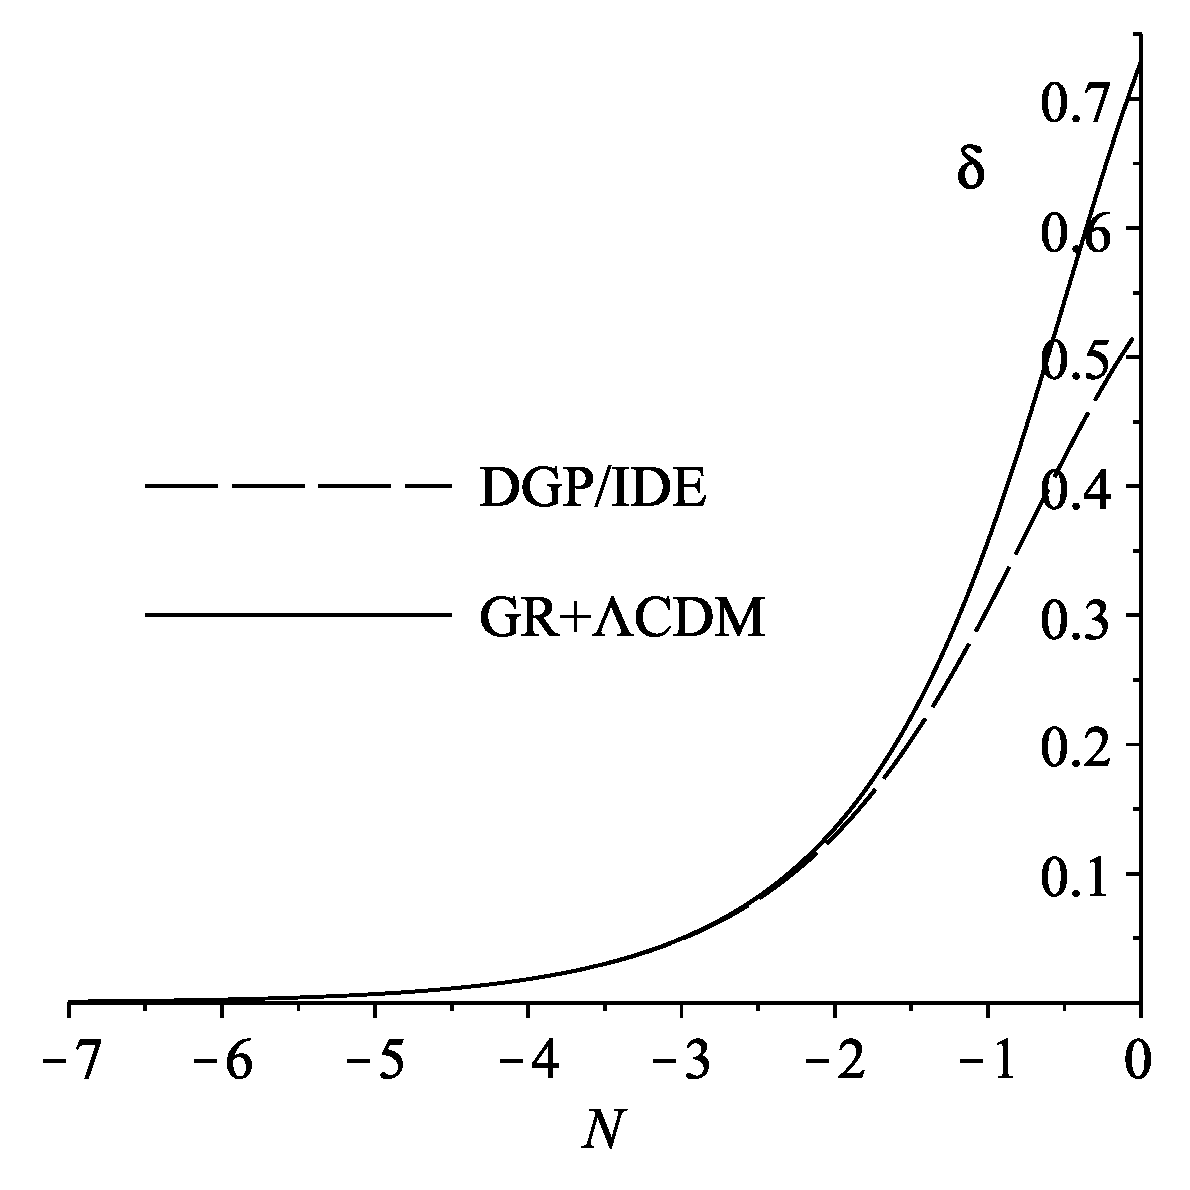
\includegraphics[width=0.49\columnwidth]{figures/dgpdeltas.eps}
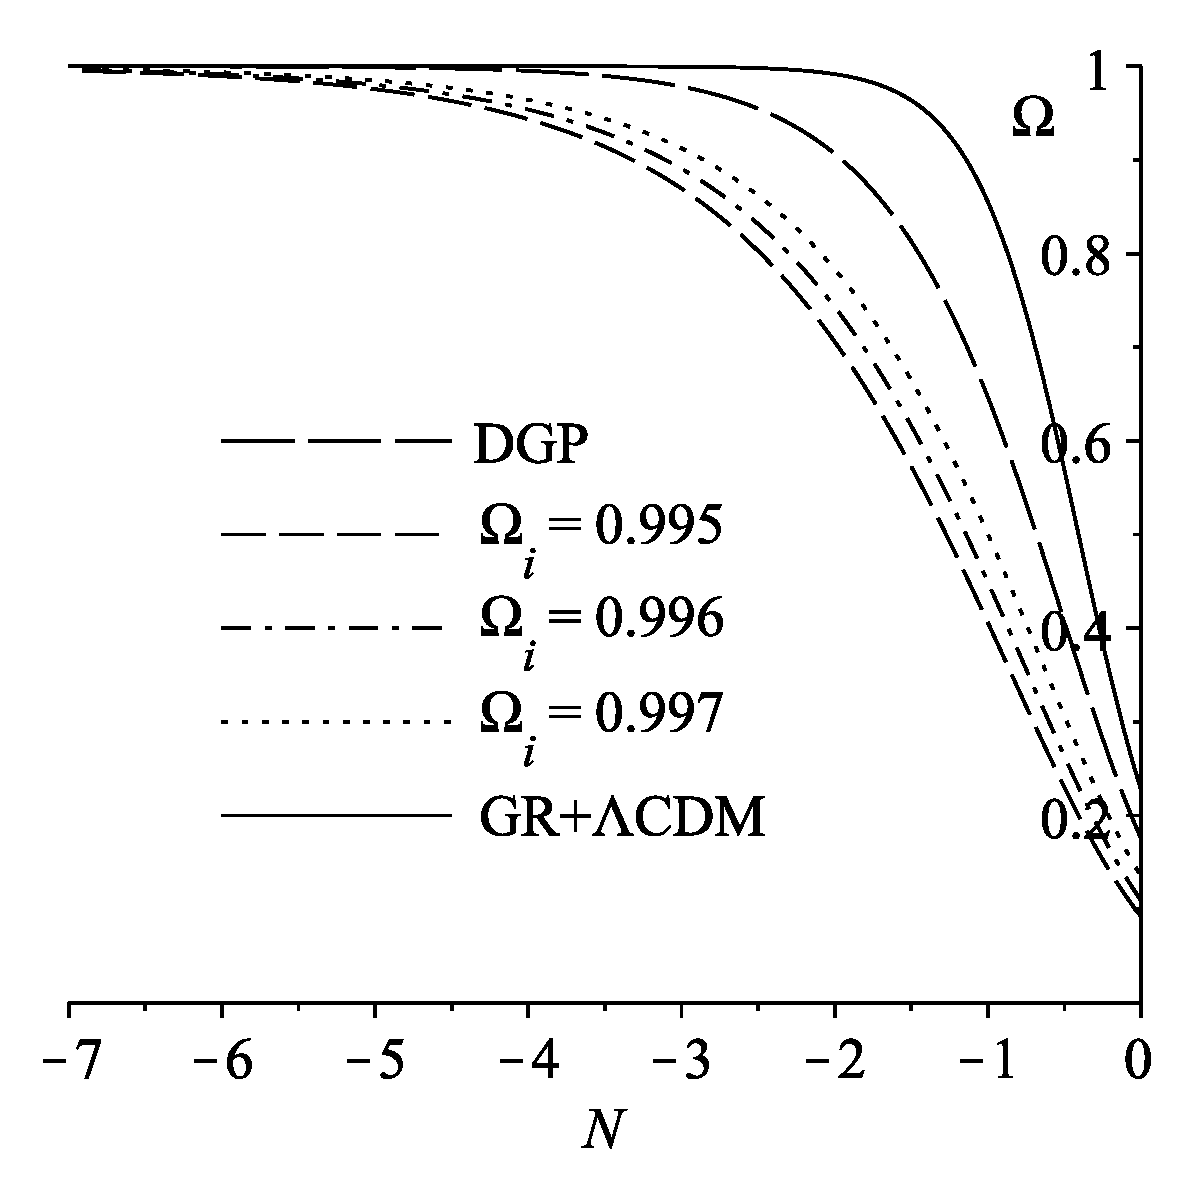
\includegraphics[width=0.49\columnwidth]{figures/dgpomegas.eps}
% For long captions include a short version for the List of Figures/Tables sections in square brackets as below.
\caption[Evolutions of $\delta$ and $\Omega$ for DGP]{Evolution of the density perturbation (left) and the density parameters (right) for the matched DGP/IDE models, each with a different $\Omega_i$,
and a GR+$\Lambda$CDM model.
\label{fig:matched}}
\end{figure}

Don't the graphs in \autoref{fig:matched} look scary? Don't worry, this is because I adapted this template from ICJS. Remember - if you are including screenshots or other raster graphics (i.e. PNG, JPEG) you should ensure that they are at least 300dpi. This will take effort on your part - most people's screens are at 72dpi.   

Vector is better (EPS or PDF) if you can manage it. If you are exporting graphs from Microsoft Excel for example, place the chart in its own sheet and print it to PDF. Then, using Acrobat or similar, crop the whitespace off the PDF. This is the most reliable way I have found to include vector graphics from Microsoft Office.







% To include math symbols in things with hyperlinks you need to specify an alternative plain text version for the bookmark using \texorpdfstring as below:
\section{A section with math symbols, eg. \texorpdfstring{$\Lambda$}{Lambda}CDM}
test test test test test test test test test test test test test test test test test test test test test test test test test test test test test test test test test test test test test test test test
test test test test test test test test test test test test test test test test test test test test test test test test test test test test test test test test test test test test test test test test
test test test test test test test test test test test test test test test test test test test test test test test test test test test test test test test test test test test test test test test test
test test test test test test test test test test test test test test test test test test test test test test test test test test test test test test test test test test test test test test test test


\chapter{Introduction} \label{chap:introduction}

\section{Overview}

Stock markets are often thought to be irrational or in some cases random,
which suggests that markets are not made based on fundamental factors alone.
In a 1996 speech, former Federal Reserve chair, Alan Greenspan questioned ``... how do we know when irrational exuberance has unduly escalated asset
values ...'' \parencite{greenspan1996}, suggesting that there may be
psychological factors that affect markets such as positive feedback loops.\\
The intended audience for such a project can vary from the institutional to
the retail investor to identify opportunities in the market by using only
publicly available data rather than proprietary information.

\section{Aims}

This project aims to produce an artificial intelligence model that
attempts to predict the following day's price of a stock index. This will
allow the project to research if a stock index's price can be predicted
from the day prior; the factors which affect a stock index's price and which
factors are most important in predicting a stock index's price.

\section{Objectives}

The objectives are as follows:
\begin{itemize}
    \item Identifying key factors that can affect stock market performance.
    \item Collecting above mentioned factors, where the historical data is publicly available and free to use (either public domain, non-commercial licenses, etc).
    \item Transforming collected data into normalised, or otherwise modified, data that can easily be used to identify patterns, either by humans or by computational neural networks.
    \item Identifying and applying correct techniques to train a computational neural network (or other suitable technology) to understand which factors are most important when predicting stock market performance.
    \item Filtering through training data to ensure there are no biases in play.
    \item Ensuring that the network will be efficient enough to be trained on hardware that is available today, and if possible on consumer hardware such as Nvidia RTX 3000 series GPUs.
    \item Understanding outputs of the computational neural networks and presenting the output data learned in a way that is clear.
    \item Interpreting overall results to identify if it is possible to predict a stock market's index direction and/or price for any given day
    \item Evauluating the results to identify accuracy, limitations and biases
\end{itemize}

\section{Constraints}
\begin{itemize}
    \item May be difficult / expensive to get historical data
    \item May be difficult / expensive to get reliable data
    \item Access to currently publicly available data may be removed, or otherwise unavailable
    \item May not have the correct technical skills to sufficiently carry out the projects
    \item May not have sufficient time to carry out the full objectives of the project
    \item Hardware available may not be feasible to run / train complex neural networks on
\end{itemize}

Even if the project was successful for now, it may not be suitable for these reasons:
\begin{itemize}
    \item May not work in extreme market events
    \item May not work if new market measures are placed
    \item May not work if new economic measures are placed
    \item Access to reliable data may be restricted, removed or otherwise unavailable in the future
\end{itemize}

\providecommand{\keywords}[1]{\textbf{\textit{Keywords.}} #1}

\chapter{Literature Review} \label{chap:literature-review}
\keywords{artificial intelligence, stock market}
\section{Introduction}
As the world advances in technology, an increasing number of decisions are dependent on computational models; including financial decisions. This includes, but is not limited to, decisions for money management, risk management, economics, and investing.
This literature review will discuss: the feasibility of predicting stock market prices; different artificial intelligence research methods used in financial modelling, particular those that relate to investing and stock market indices; and the different input features used in these models.

\section{Feasibility of predicting stock market index prices}
\subsection{Efficient Market Hypothesis}
Over the year,  many people have attempted to predict stock markets in order to profit from price movements as they occur. However, some have theorised that it is not possible to accurately predict prices due to the there being an innumerable number of factors that can affect a stock market, and these factors would already be a function of the current market's price, therefore make it impossible to forecast the price. \parencite[1]{theoryofspeculation} This is the basis of the Efficient Market Hypothesis, where an asset price fully reflects the information that is available at any given time.

\subsection{Empirical evidence of market (in)efficiencies}
A 1973 book explains the term `random walk' as ``A random walk is one in which future steps or directions cannot be predicted on the basis of past actions``, and continues to describe how when applied to the stock market that ``short-run changes in stock prices are unpredictable. [and] Investment advisory services, earnings forecasts, and complicated chart patterns are useless'' \parencite[24]{burton_gordon_malkiel_2016}.
A reflection paper by the same author 30 years on, attempts to validate that the efficient market hypothesis still holds true in the 21st century by comparing actively managed funds to tracker funds: suggesting that markets are likely efficient, due to the fact that most actively managed funds are outperformed by a index tracker fund that follows the S\&P 500 index; the data presented suggests that most experts (68\% to 90\% over various time periods) cannot outperform the index whether it be from a one year, three year, five year, ten year or twenty year holding period leading up to 31st December, 2003 \parencite{reflections30years}. The author suggests that if markets were inefficient, fund managers should easily be able to outperform the index.

In order to prove, or disprove, the Efficient Market Hypothesis, many studies have been carried out with varying results. In this literature review we will focus on the US markets and the different results the studies have found. Using data from 1964 to 2003 for the US stock market, one study has found markets to be efficient using a threshold autoregressive model and a unit root process \parencite{narayan2006behaviour}. Another empirical look into equity premium prediction, that looks specifically at the US S\&P 500 index, using various regression models with additional variables described such as dividends, earnings price ratio, book value, net issuing activity and more has concluded that ``the equity premium has not been predictable'' \parencite[abstract]{goval_welch_2004} which would agree with the efficient market hypothesis.

% A study with a more up-to-date dataset, that looks at 350 companies listed on the London Stock Exchange and S\&P 500 between 2007 to 2013, using an auto-regressive moving average model can be used to calculate mid-long term returns on the LSE and monthly/annual on SP500. https://doi.org/10.1016/j.physa.2016.03.006

However, other recent studies have suggested the efficient market hypothesis may not hold true. A paper that looks into returns of the US Dow Jones Industrial Average (DJIA) index from 1928 to 2012 showed that while for autocorrelation tests on daily and weekly intervals suggest market efficiency, the same cannot be said for monthly and annual intervals (although the degree of correlation is low). Furthermore, the paper posits that autocorrelation tests are not sufficient to determine dependencies, and puts forwards another type of test called `run tests' to show that markets are also inefficient in daily and weekly intervals \parencite{sewell_2012}. Another paper that analyses data from 1999 to 2007 of various markets, including the US as well as other developed and developing countries, using a unit root process has stated that their findings show that ``real stock price indices are stationary processes that are inconsistent with the efficient market hypothesis'' \parencite[1]{LEE201049}.

%file:///C:/Users/alvie/Downloads/IJMFA70307_Rossi_LR_CA3.pdf

%https://etalpykla.lituanistikadb.lt/object/LT-LDB-0001:J.04~2015~1447771572718/J.04~2015~1447771572718.pdf


\section{Types of artificial intelligence methods used}

\subsection{Description of artificial intelligence methods}
Various artificial intelligence methods have been utilised in order to predict daily direction as well
as price of stock markets, the following are described here:
\begin{itemize}
    \item Multilayer Perceptrons (MLPs)
    \item Convolutional Neural Networks (CNNs)
    \item Support Vector Machines (SVMs)
    \item Long Short Term Memory (LSTM)
    \item Hybrid approaches
\end{itemize}

\subsubsection{Multilayer Perceptrons (MLPs)}
Multilayer Perceptrons (MLPs - \autoref{fig:multilayer-perceptron}) are a class of artificial neural networks. They contain multiple layers
of perceptrons, including an input layer, one or many hidden layers and an output layer. They are
feed-forward networks meaning that data is only passed to the next layer and does not move backwards.
It is an example of a supervised neural network as labelled data is used in training.

\begin{figure}[hbt!]
    \centering
    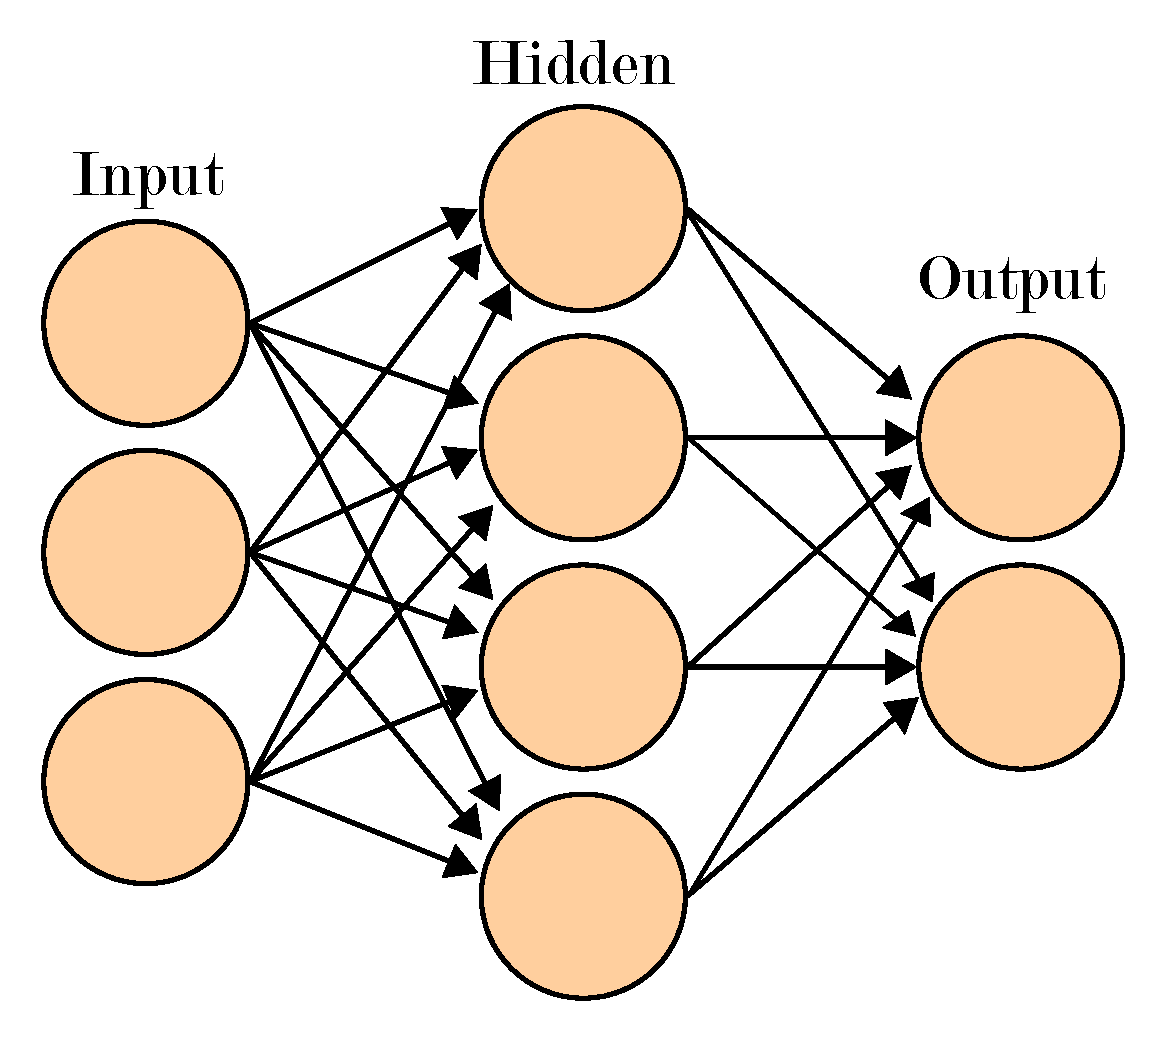
\includegraphics[width=0.4\columnwidth]{figures/multilayer-perceptron.pdf}
    \caption[Diagram of a Multilayer Perceptron]{Diagram of a Multilayer Perceptron; adapted from Artificial neural network.svg, Wikimedia, Cburnett}
    \label{fig:multilayer-perceptron}
\end{figure}
\FloatBarrier

\subsubsection{Convolutional Neural Networks (CNNs)}
Convolutional Neural Networks (CNNs - \autoref{fig:convolutional-neural-network}) are a class of artificial neural networks. They contain
multiple layers; including an input layer, one or many convolutional and pooling layers, and an
output layer. The convolutional and pooling layers are inspired by biological processes; each
layer extracts and summarises certain features and convolves the input and passes to the next
layer. The pooling layers are using to reduce the spatial size of the data by combining outputs
in order to optimise the network for performance.

They are feed-forward networks meaning that data is only passed to the next layer and does
not move backwards. It is an example of a supervised neural network as labelled data is used
in training.

\begin{figure}[hbt!]
    \centering
    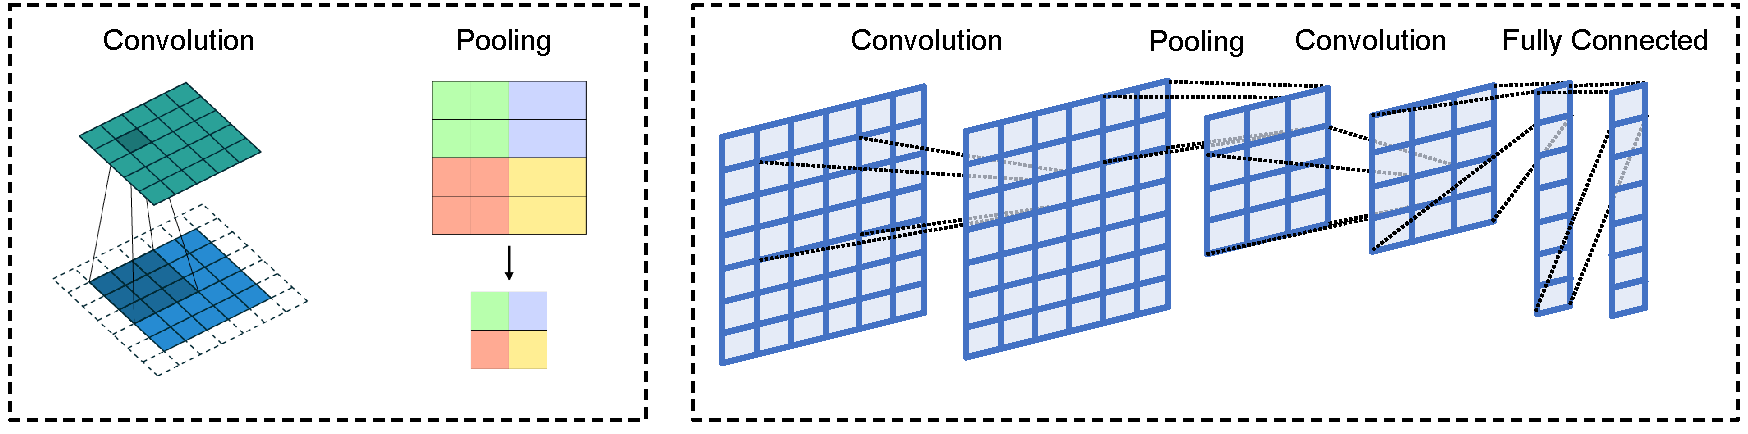
\includegraphics[width=0.75\columnwidth]{figures/convolutional-neural-networks.pdf}
    \caption[Diagram of a Convolutional Neural Network]{Diagram of a Convolutional Neural Network; \parencite{Maier2019}}
    \label{fig:convolutional-neural-network}
\end{figure}
\FloatBarrier

\subsubsection{Support Vector Machines (SVM)}
Support Vector Machines (SVMs - \autoref{fig:support-vector-machines}) are a class of machine learning models that are used in classification
of data. In this model, the training data is used in order to identify a decision boundary, known as
a hyperplane that separates the classifications of data. It is an example of a supervised machine
learning model as labelled data is used in training.
\begin{figure}[hbt!]
    \centering
    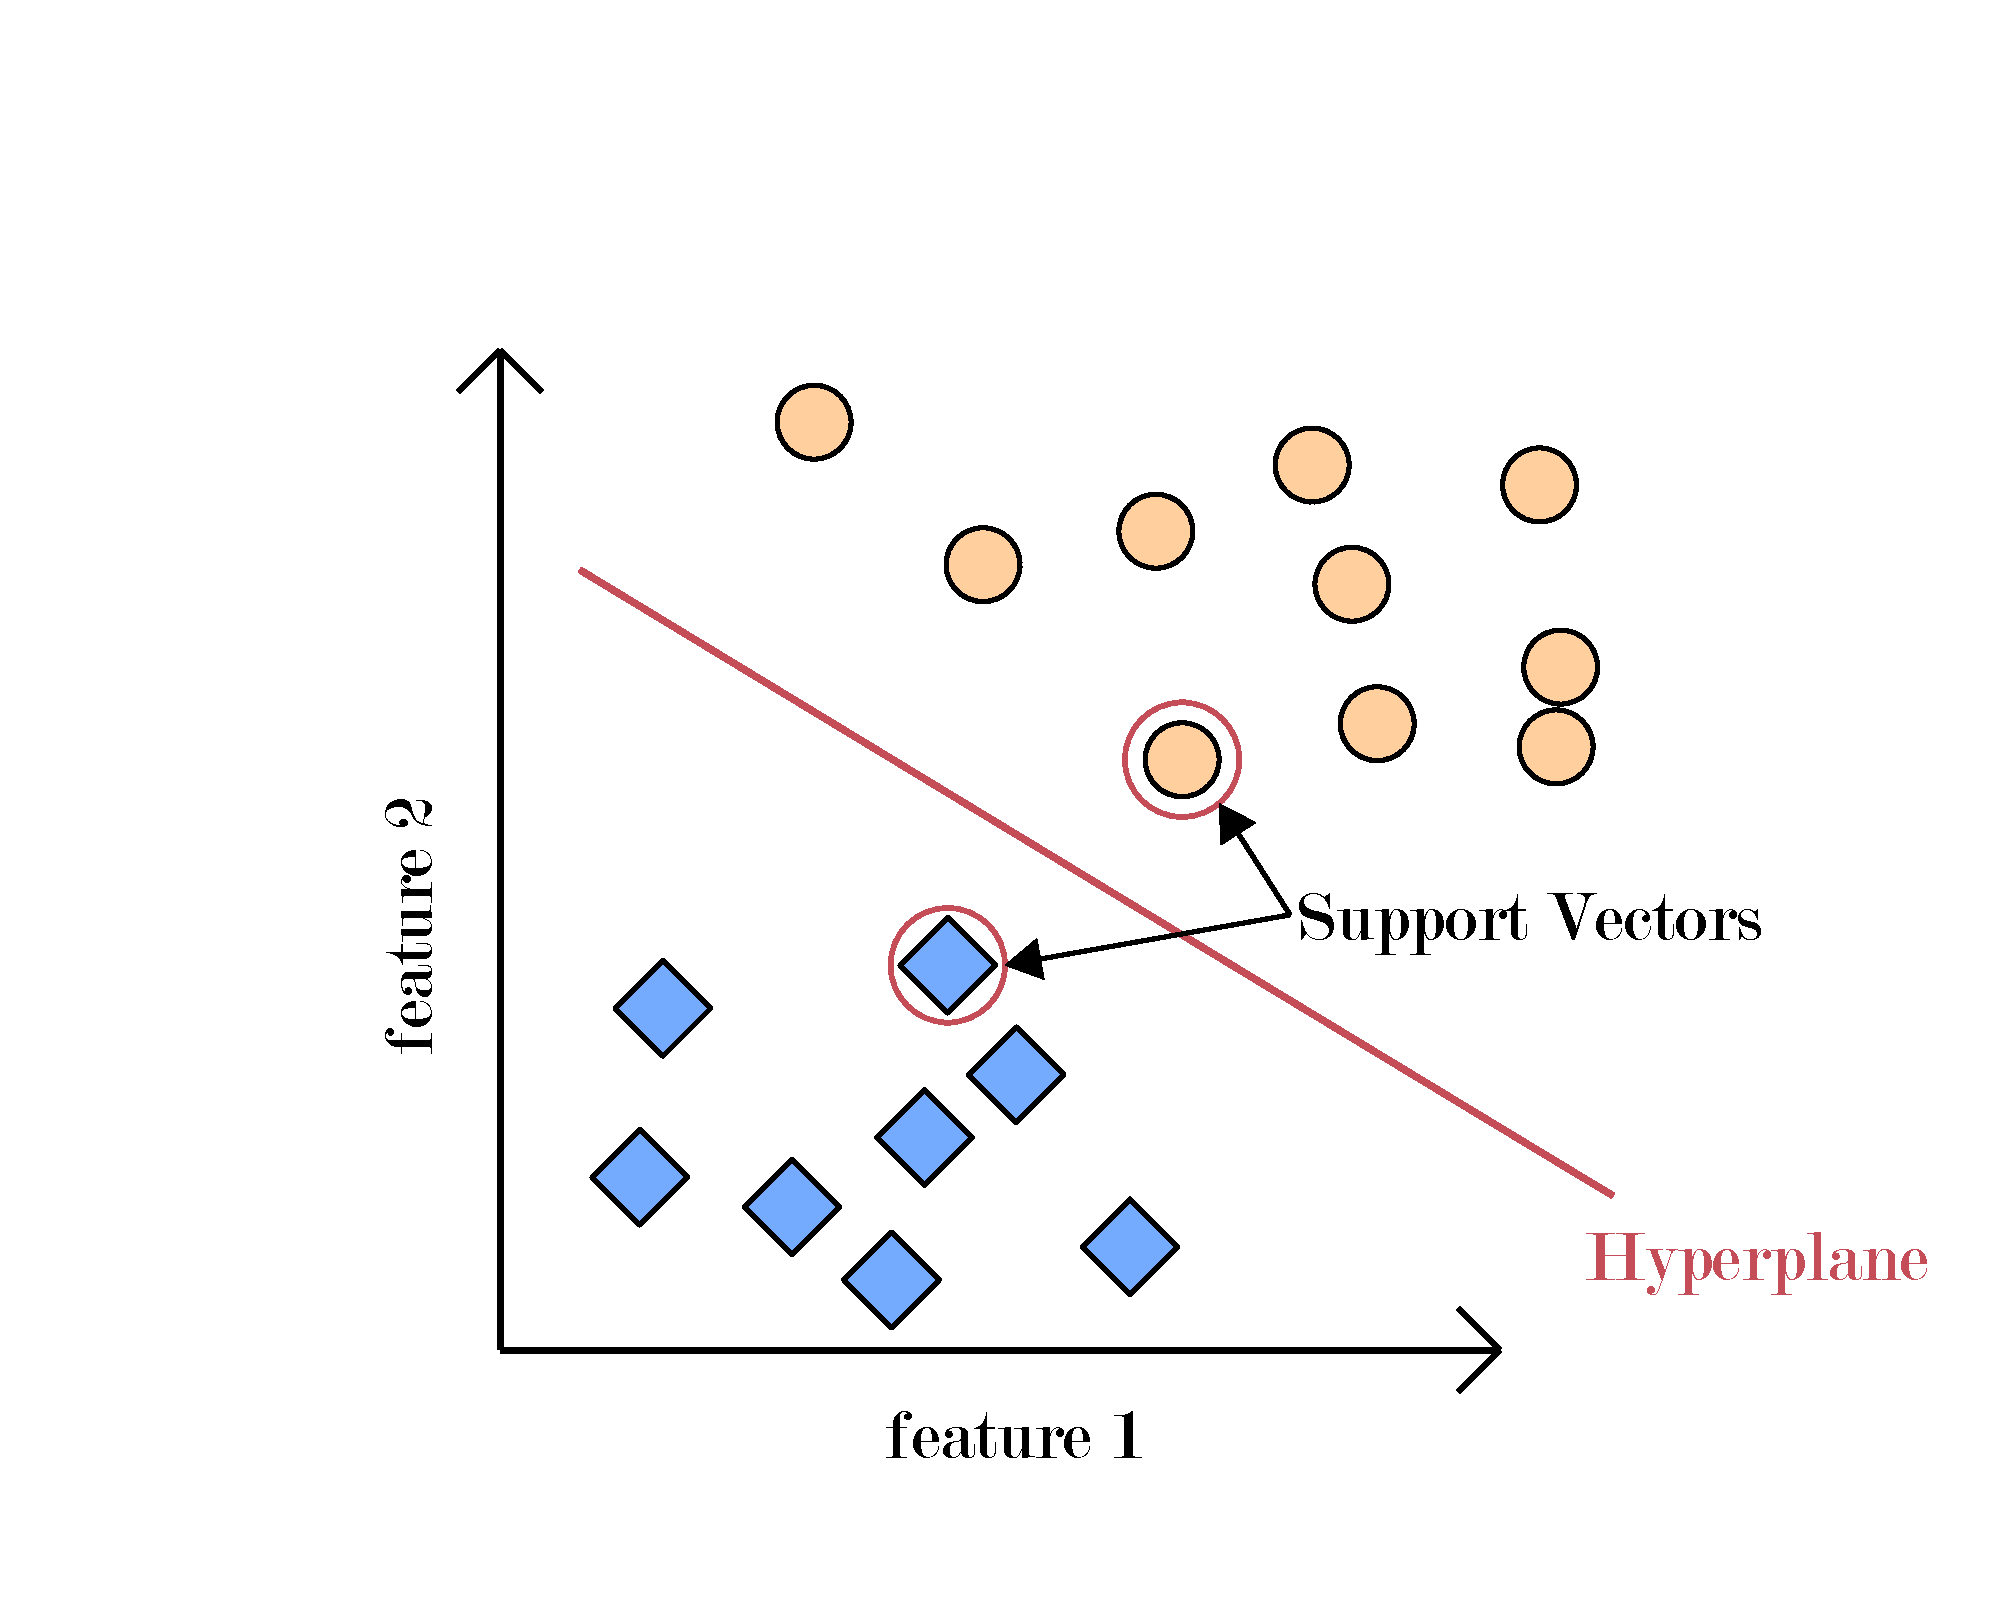
\includegraphics[width=0.6\columnwidth]{figures/support-vector-machines.pdf}
    \caption[Diagram of a Support Vector Machine]{Diagram of a Support Vector Machine}
    \label{fig:support-vector-machines}
\end{figure}
\FloatBarrier

\subsubsection{Long Short Term Memory (LSTM)}
Long Short Term Memory (LSTM - \autoref{fig:long-short-term-memory}) is a class of artificial neural networks. They are recurrent
networks meaning that data is not necessarily fed-forward as they allow for loops within the
network. LSTMs contain cells with `gates' that allow them to keep context and control the flow of data,
as well as make decisions to keep or discard data in order to make predictions. It is an example of a supervised neural network as labelled data is used in training.

\begin{figure}[hbt!]
    \centering
    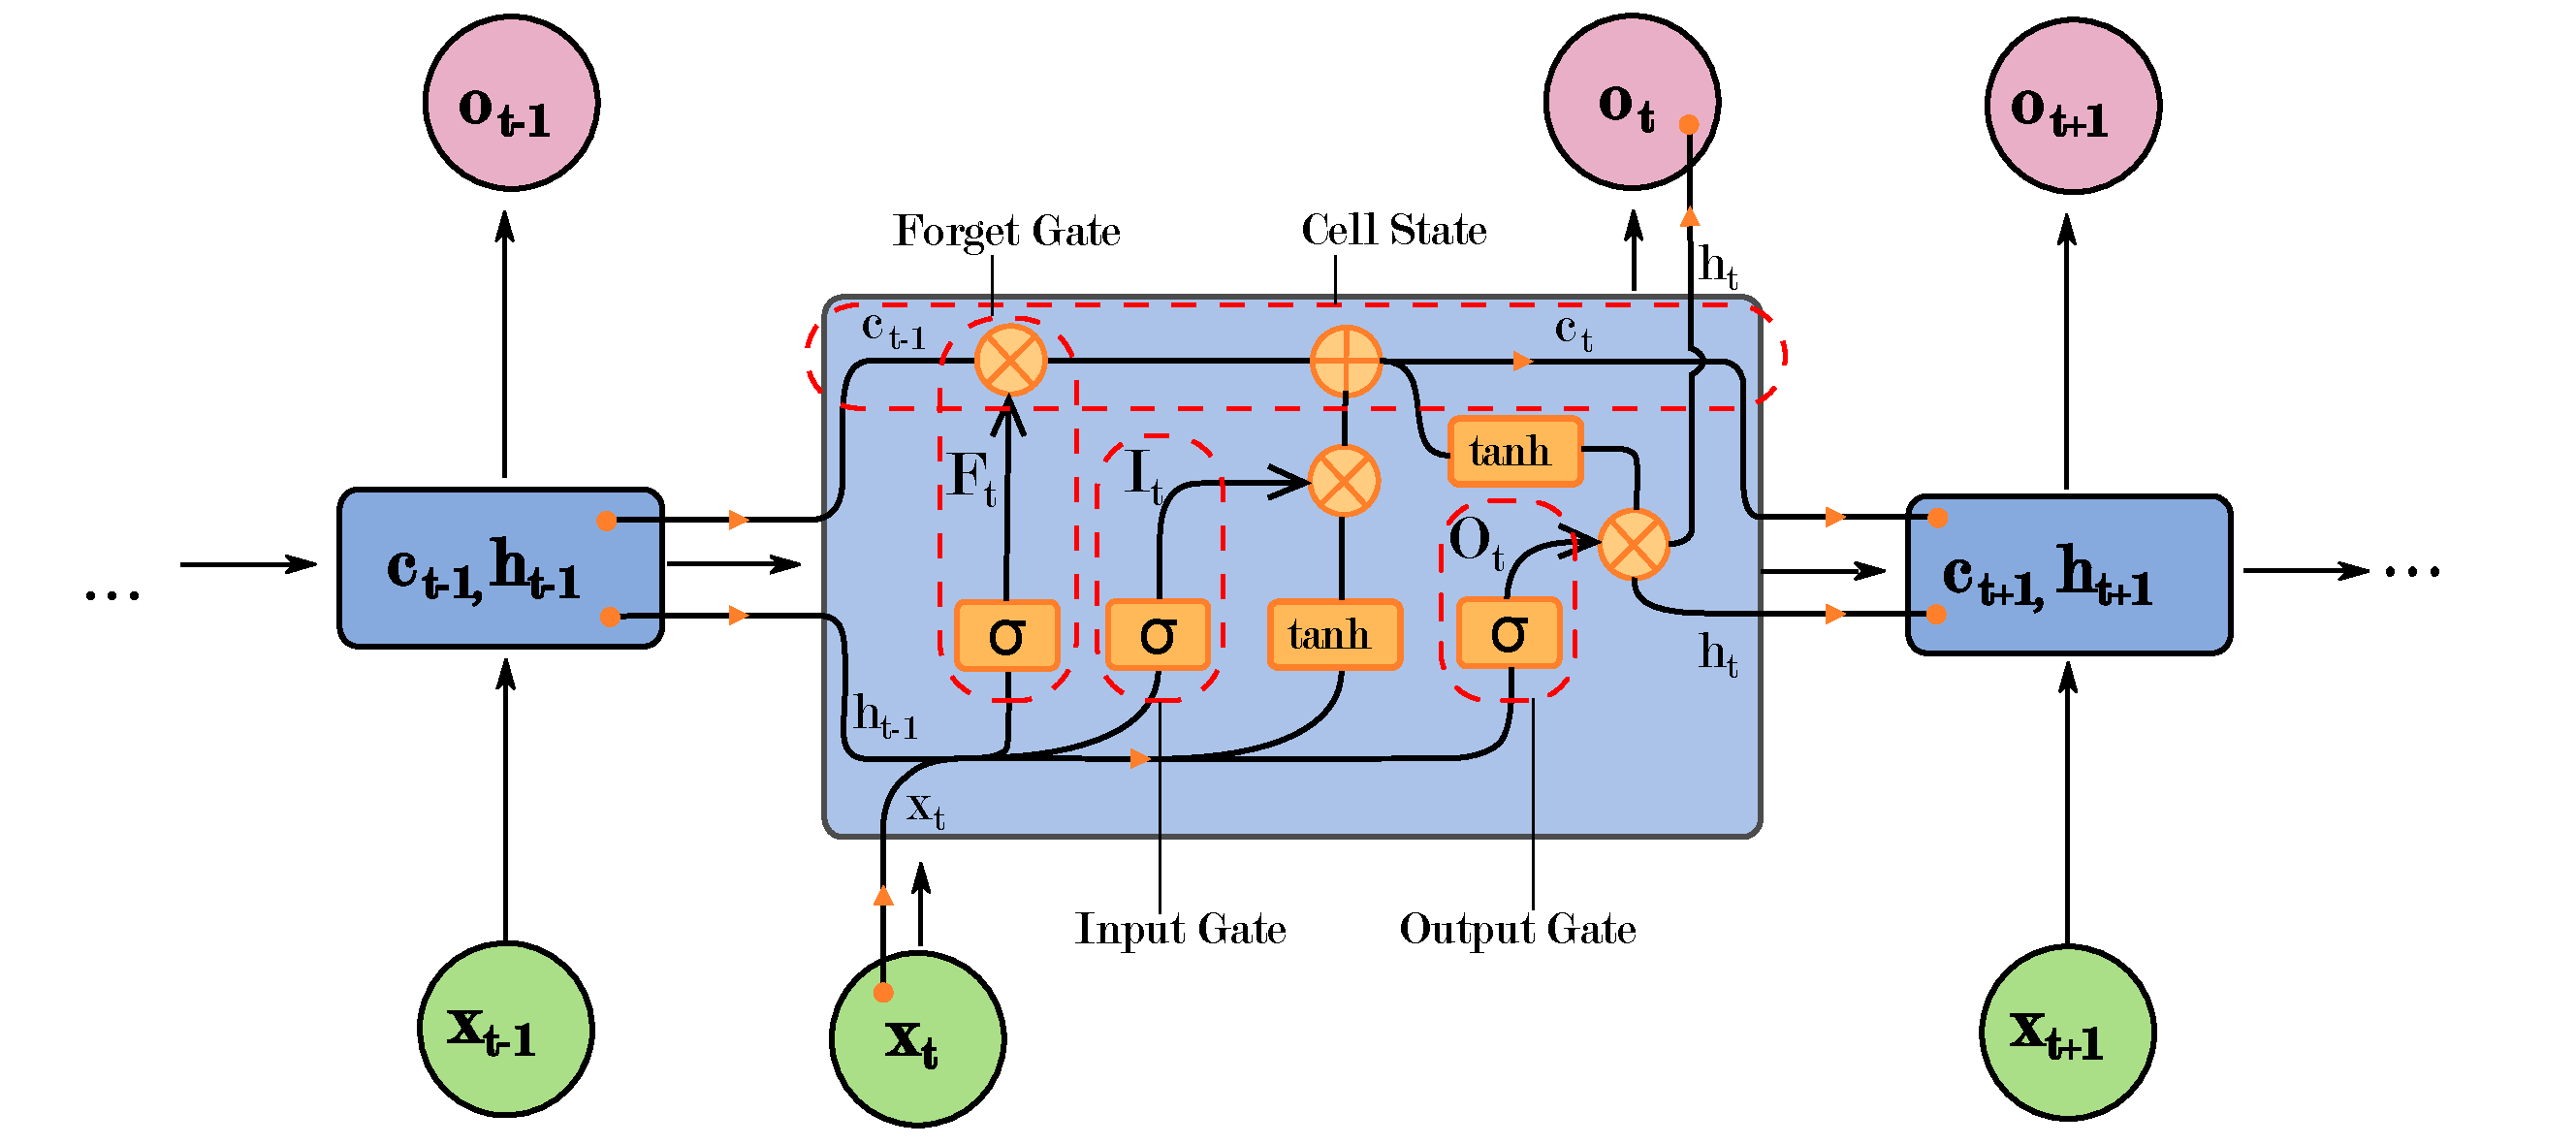
\includegraphics[width=\columnwidth]{figures/long-short-term-memory.pdf}
    \caption[Diagram of a LSTM Unit]{Diagram of a Long Short Term Memory Unit; adapted from Long Short-Term Memory.svg, Wikimedia, fdeloche}
    \label{fig:long-short-term-memory}
\end{figure}
\FloatBarrier

\subsubsection{Hybrid Approaches}

Hybrid approaches can be utilised in order to overcome shortcomings in certain models. A hybrid
approach can utilise any number of different models; for example a CNN-LSTM hybrid model will use
CNN and LSTM layers as a CNN may be a good model for classification problems, an LSTM is better
suited to time series data.

\subsection{Artificial intelligence methods used in previous studies}

Different studies have utilised different artificial intelligence models to predict the price of stock market indices, with varying degrees of accuracy.

One study using multilayer perceptrons (MLP) to predict the daily direction of an exchange traded fund (ETF) that tracks the US S\&P 500 stock market index suggests that the model has an accuracy of up to 60\% \parencite{zhong2019predicting}. Whereas another study has suggested they can predict the price, not just direction, of the same stock market index with an accuracy of 76\% using support vector machines (SVMs) and reinforcement learning \parencite{shen2012stock}. As there is a difference of 16\%+ in of accuracy in the same stock market index (S\&P 500), and the higher accuracy model suggests that support vector machines may provide an improvement over feed-forward neural networks such as MLPs. Another study comparing the performance of MLPs and SVMs agrees that SVMs are superior as, even though both models were able to predict the direction of the S\&P 500 index, the MLP model had a maximum error difference of 15\% over a 45 day period, whilst the SVM model had a maximum error difference of 6\% in their test cases\parencite{comparisonregannsvm}. %interesting input features, mention in next part
This is further supported by another study comparing various artificial intelligence methods on the Indian Nifty50 index with the SVM model outperforming a back-propagation neural network model, which is somewhat similar to the MLP model, by 5.51\% \parencite{kumar2006forecasting}.

Further studies have been done on using hybrid approaches to predict stock markets. One study using an approach with a convolutional neural network (CNN) and three long short-term memory (LSTM) networks found that the accuracy of predicting weekly directions of the S\&P 500 index was 66.6\%, which was greater than with SVMs or CNNs alone,  with those models achieving 62.0\% and 59.3\% respectively \parencite{hao_gao_2020}. Another study agrees with these findings, with their results also suggesting a model built with CNNs and bi-directional LSTMs are able to outperform SVMs \parencite{noveldeepcnnbilstm}. However, the same cannot be said for all types of hybrid neural network models; one study comparing MLPs and hybrid networks on the US Nasdaq index has found that the MLP performs better, albeit slightly with a difference of 0.26\% in mean absolute deviation, than an approach with a hybrid model of MLP and Generalized Auto-Regressive Conditional Heteroskedasticity (GARCH) \parencite{GURESEN201110389}.

\section{Input features for intelligence methods}
The studies mentioned in the previous section use different input features for their studies;
where the amount of input features ranges from just a single type of input to many various macro-economic factors.
One of the hybrid approaches has only stated using the `daily closing price dataset of the S\&P 500 index' in their CNN-LSTM model
\parencite{hao_gao_2020}.
Another study using the hybrid approach slightly expands on this by using additional factors related to the index:
the opening and closing prices of the S\&P 500 index, the low and high prices of the day, and the trading volume
\parencite{fitriyaningsih2019implementation,THAKKAR2020106684, hu_tang_zhang_wang_2018}. However, these studies have not considered any macro-economic factors. One study expands on this further by also including other indexes across the world as inputs, as well as various currency rates in addition to commodities such as oil and metals \parencite{shen2012stock}. Other studies expand on this further, for example one study with 27 input features also includes US Treasury yield rates and bond yields \parencite{comparisonregannsvm} and another looks into additional factors for a total of 60 input features including certificate of deposit rates, and term and default spreads \parencite{zhong2019predicting} - though the latter study explains that with principal component analysis, the model peaked in terms of accuracy with 31 input features.

\section{Conclusion}
To conclude, there are differing opinions on whether markets are efficient, and therefore whether they are predictable. Some economists use the fact that experienced fund managers are rarely able to beat the market as proof that markets are efficient, and there are studies that agree with this hypothesis. However, there are also other studies that disagree presenting their findings that show there is some evidence of market inefficiencies in either the short term or long term.

Regardless of markets being efficient or not, numerous artificial intelligence methods — including MLPs, SVMs, CNNs as well as hybrid approaches using CNNs and LSTMs -- have been employed to varying degrees of success. While some studies look at predicting just the direction, and others attempt to predict the price, most have claimed to be able to do so with above 50\% accuracy. From the studies researched here, it can be assumed that in general hybrid approaches involving CNNs and LSTMs outperform SVMs, which outperform MLPs.

These studies use a diverse set of input features in order to build their models, with some using features only directly related to the index and some using extended datasets including inputs from macroeconomic sources in order to build models that take account external factors that may affect the index's price, though there is evidence to suggest that not all of the input features are required to build a good model to predict the price of an index.
\chapter{Research Questions} \label{chap:research-questions}


\section{Predicting a stock market index's direction}
\textbf{Question} Is it possible to accurately predict a stock market index's (S\&P 500) direction for
the following day with an artificial intelligence model?\\
\textbf{Sub Questions}
\begin{itemize}
    \item If so, what is the accuracy of the model?
    \item If not, what limitations affected the model to cause it to be inaccurate?
    \item Can the findings of this question be used to prove/disprove the efficient market hypothesis?
\end{itemize}
\textbf{Importance} The findings from this research question will have significant impact in making
investment and trading decisions for participants of the market, potentially giving indicators of
when to buy / sell into the stock market in order to outperform the market. Furthermore, depending
on the accuracy of the model, it may be able to be used as evidence for or against the efficient
market hypothesis.

\section{Optimal amount of historical data as input}
This question assumes that it is at least somewhat possible to accurately predict the stock market index's
direction/price based on literature review and other studies.\\
\textbf{Question} How do different lengths of time as history for the input in the training data affect the model?\\
\textbf{Sub Questions}
\begin{itemize}
    \item What is the ideal length of time to be used in the training data?
    \item What are potential reasons for this length of time being the most useful?
\end{itemize}
\textbf{Importance} The findings from this research question will allow optimal algorithms /
models to be created in order to avoid wasting computational time that may cause the model to 
not improve, or even decrease in accuracy. Furthermore, this will be of help to participants of
the market to make better informed manual decisions by understanding which time horizons to look
at.

\section{Most important input features}
This question assumes that it is at least somewhat possible to accurately predict the stock market index's
direction/price based on literature review and other studies.\\
\textbf{Question} What are the most important input features that affect the model?\\
\textbf{Sub Questions}
\begin{itemize}
    \item How much do each of these input features contribute to the model?
    \item Do any of the input features identified have negligible impact to the model?
    \item What are the potential reasons these features do / do not impact the model?
\end{itemize}

\textbf{Importance} The findings from this research question will allow optimal algorithms /
models to be created in order to avoid wasting computational time that may cause the model to 
not improve, or even decrease in accuracy. Furthermore, this will be of help to participants of
the market to make better informed manual decisions by understanding which factors to look
at.
\chapter{Research Design} \label{chap:research-design}
\section{Research methodology}
The research methodology is one based on the literature review (\autoref{chap:literature-review});
the research already carried out in other studies
informed the decision making process behind the requirements of the supporting artefact. Various artificial
intelligence models have been analysed and critiqued; as well as the input features used within these models.

These aspects combined are used to inform the variables - such as model used, input features
(and their sequence lengths of historical data) - to experiment with to better understand which variables are most important
and have the ability to provide the most accurate results.

\section{Research process}
\subsection{Comparison of AI models in previous studies}
From the literature review, various AI models were identified. These include Multilayer Perceptrons (MLPs),
Convolutional Neural Networks (CNNs), Support Vector Machines (SVMs), Long Short Term Memory (LSTM) and hybrid
approaches. From this, we can understand which models can have greater accuracy. The review has found a hybrid
approach has the greatest accuracy. CNNs and SVMs have a similar degree of accuracy and generally outperform MLPs.

\begin{table}[h]
    \centering
    \begin{tabular}{|p{50mm}|p{40mm}|p{35mm}|}
        \hline
        Artificial Intelligence Model & Ease of Implementation & Accuracy of Output \\
        \hline\hline
        Multilayer Perceptrons & 5 & 3 \\
        Convolutional Neural Networks & 3 & 4 \\
        Support Vector Machines & 3 & 4 \\
        Hybrid (CNN + LSTM) & 2 & 5 \\
        \hline
    \end{tabular}
    \caption[Table rating different AI models]{Table rating different AI models on a scale of 1 to 5 based on ease of implementation as well as accuracy}
    \label{tab:research_model_comparison}
\end{table}
\FloatBarrier

\subsection{Input features used in previous AI models}
Currently, based on the studies in the literature review, it is difficult to suggest which input features
are most important for an accurate output. This is due to the studies using more complex datasets as input
features generally use a different research model.

This is one of the primary research questions identified, and this project intends to answer this question.
The previous studies use the following input features; a subset of the features will be used and compared
within this project. 
\begin{itemize}
    \item Daily Closing Price
    \item Low Price
    \item High Price
    \item Volume
    \item Currency Rates
    \item Commodities (e.g. Oil)
    \item Treasury Rates
    \item Stock indices of other countries
    \item Individual Stocks
    \item Certificate of Deposits
    \item Term spreads
\end{itemize}

\section{Expected research outcomes}
As CNN+LSTM hybrid approaches have already been proven in previous studies to be an accurate research model,
this model will be researched within the artefact of this project. However, the effect of different input
features on a single research model has not been well identified. This will be a primary area of focus for
the supporting artefact to look into. The academic novelty exists within the fact that
there is a unique set of input features on the CNN+LSTM model or other well-performing model; and also finding the optimal sequence and
combination of input features. Ideally, this will allow the supporting artefact to have greater than
60\% accuracy in predicting the daily price direction.

\section{Requirements of the artefact}
\subsection{Functional requirements}
Based on the literature review, the most accurate models for predictting stock prices had an accuracy of
approximately 60\% \parencite{zhong2019predicting}. While there is an example of a study shown with a greater
accuracy of 76\% \parencite{shen2012stock}, another similar study places the accuracy of the model at 59.3\%
- albeit for weekly predictions rather than daily \parencite{hao_gao_2020}; thus 60\% is considered the
current baseline.\\
Also, due to the fact that this research project attempts to identify the most important input features, as
well as the sequence length, they are key requirements of this project.\\
Predicting the exact return (daily relative price change) per day is an optional requirement due to two
reasons: it does not significantly help market participants compared to knowing the direction alone; and
it may be more cumbersome / time-consuming for a relatively low significant output for end users.
\subsubsection{Necessary requirements}
\begin{itemize}
    \item Predict daily price direction with 60\%+ accuracy
    \item Identify which input features are most important
    \item Identify what sequence length (number of days of history of each input feature) is optimal
    \item Present charts of accuracies and losses of each model
\end{itemize}

\subsubsection{Optional requirements}
Based on the literature review, a study suggested it had been able to accurately predict prices with a mean
absolute deviation of 2.516\% on the testing data set when compared to the true price.
\begin{itemize}
    \item Predict daily price return with a mean absolute deviation of 2.5\% or lower
\end{itemize}
\subsection{Non-functional requirements}
The results from the artefact are not time critical due to there being a large time period 17 hours and 30 minutes
between market close (4:00 PM ET) and market open (9:30 AM ET) of stock exchanges in the USA; however this
may not be ideal for users thus the following non-functional requirements have been identified.

\subsubsection{Necessary requirements}
\begin{itemize}
    \item The artefact should take less than one minute to run per model chosen (on modern Nvidia GPUs)
\end{itemize}

\subsubsection{Optional requirements}
\begin{itemize}
    \item Front-end application that allows users to input features and sequence lengths to train different models
    \item User-facing documentation for artefact
\end{itemize}
\chapter{Artefact Design} \label{chap:artefact-design}
\section{Development decisions}
\subsection{Software development methodology}
In the software development life cycle there are various stages: requirements gathering, analysis, design,
development, testing, deployment and maintenance.\\
The Agile software development methodology will be utilised in this project; and this project will be separated
into various iterations of design, development, and testing. This will allow for a more flexible approach to
the task and the ability to make changes as the project progresses without requiring additional time and effort
to fully test and deploy an inaccurate or unsuitable artefact.
There are various iterations that will be used to gradually improve to a final version that will be used to
form answers for the research questions.
\begin{figure}
    \centering
    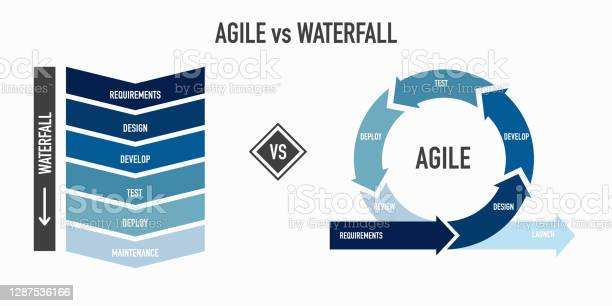
\includegraphics[width=\columnwidth]{figures/development_methodologies.jpg}
    \caption{A comparison of the Agile and Waterfall methodologies (source: iStock, iam2mai)
    (replace as there is a copyright)}
    \label{fig:development_methodologies}
\end{figure}
\FloatBarrier

\subsection{Software languages and libraries}
\subsubsection{Programming Language}
Python has been chosen to be used in this project as it is ubiquitous for artificial intelligence related
tasks. There are many resources readily available for Python with regards to its usage on artificial
intelligence models and neural networks. There are various Python libraries for machine learning applications
such as Tensorflow, an `end-to-end open source machine learning platform' created by Google as well as
PyTorch, ` open source machine learning framework' created by Facebook's AI Research Lab.

\subsubsection{Python libraries for machine learning}
As mentioned in the previous section there are various machine learning libraries for Python. Currently, the
most popular is Tensorflow and has the most resources available.
However, the usage of PyTorch has accelerated over the past years and is quickly becoming the preferred
library as it is considered to be more `pythonic' and often quicker to train neural networks.

Tensorflow will be used in the project due to its current ubiquity in this task, especially surrounding
its applications for financial forecasting. However, PyTorch may be chosen for future iterations if
the performance of Tensorflow is found to be insufficient and the performance of PyTorch is found to be
greater.

\section{Input features chosen and data collection}\label{ssec:input_feature_chosen}
The input features chosen are an amalgamation primarily based on those found in the literature review.
However, there are several input features that have previously not been used in such as repurchase agreements
data, as well as sentiment data, etc. This represents a first time application of an existing research method
to a novel case study for many of the models.

From the literature review, the input features have been classified into four categories:
\begin{itemize}
    \item Stock market index
    \item Money availability
    \item Alternative portfolio allocations
    \item Sentiment
\end{itemize}

From this, the following sources for input features have been chosen; the reasoning are explained and the
sources for used in the data collection process are also present within this list.
\begin{itemize}
    \item Stock market index
    \begin{itemize}
        \item Closing price\\
        \textbf{Reasoning:} It is believed that a sequence of closing price returns
        can be utilised to predict a future closing price\\
        \textbf{Source:} Yahoo Finance - SPY Historical Data:\\
        https://uk.finance.yahoo.com/quote/SPY/history
        \item Volume\\
        \textbf{Reasoning:} It is believed that the amount of stock traded can indicate
        confidence in that stock market index and potentially future price movements\\
        \textbf{Source:} Yahoo Finance - SPY Historical Data:\\
        https://uk.finance.yahoo.com/quote/SPY/history
        \item Volatility (based on VIX)\\
        \textbf{Reasoning:} It is believed that the volatility in the stock market can potentially
        indicate future price movements\\
        \textbf{Source:} Yahoo Finance - VIX Historical Data:\\
        https://uk.finance.yahoo.com/quote/\%5EVIX/history
    \end{itemize}
    \item Money availability
    \begin{itemize}
        \item M1 Money Supply\\
        \textbf{Reasoning:} It is believed that a change in total money supply circulation can affect
        the amount of money allocated to the stock market, such as with measures related to quantitative
        easing to affect stock returns\\
        \textbf{Source:} Federal Reserve Economic Data - M1 Money Supply:\\
        https://fred.stlouisfed.org/series/WM1NS
        \item GDP\\
        \textbf{Reasoning:} It is believed that the GDP can affect the money available to market
        participants and thus impact stock returns\\
        \textbf{Source:} Federal Reserve Economic Data - GDP:\\
        https://fred.stlouisfed.org/series/GDP
    \end{itemize}
    \item Alternative portfolio allocations
    \begin{itemize}
        \item Treasury Yields
        \begin{itemize}
            \item 1Mo
            \item 3Mo
            \item 1Yr
            \item 2Yr
            \item 5Yr
            \item 10Yr
            \item 20Yr
            \item 30Yr
        \end{itemize}
        \textbf{Reasoning:} It is believed that the market participants often allocate their funds
        to treasury bonds / bills / notes for a guaranteed return compared to risk in the stock market.
        A change to yields may affect the money allocated in the stock market and thus affect the
        return of the stock market index.\\
        \textbf{Source:} US Dept. of the Treasury - Treasury Par Yield Curve Rates:\\
        % \seqsplit{https://home.treasury.gov/resource-center/data-chart-center/interest-rates/TextView?type=daily_treasury_yield_curve}
        \item Effective Federal Funds Rate\\
        \textbf{Reasoning:} EFFR is the interest rate banks charge one another for overnight loans, a change in
        EFFR may affect the loans banks make / take and thus affect the money the banks have available to allocate
        in the stock market; this may affect the return of the stock market index.\\
        \textbf{Source:} Federal Reserve Economic Data - EFFR:\\
        https://fred.stlouisfed.org/series/EFFR
        \item Repurchase / Reverse Repurchase Agreements\\
        \textbf{Reasoning:} A change in utilisation of repurchase agreements may indicate if banks expect
        a greater return elsewhere and how banks are allocating money. This may have an impact on the
        return of the stock market index\\
        \textbf{Source:} New York Fed - Repo:\\
        https://www.newyorkfed.org/markets/desk-operations/repo
        \item Gold\\
        \textbf{Reasoning:} It is believed that a change in the prices of commodities such as gold may be
        an indicator of portfolio allocation changes; thus affecting the return of the stock market index\\
        \textbf{Source:} London Bullion Market Association - Precious Metal Prices:\\
        https://www.lbma.org.uk/prices-and-data/precious-metal-prices\#/table
        \item Foreign Currency
        \begin{itemize}
            \item USD-GBP\\
            \textbf{Source:} Federal Reserve Economic Data - GBP:\\
            https://fred.stlouisfed.org/series/DEXUSUK
            \item USD-EUR\\
            \textbf{Source:} Federal Reserve Economic Data - EUR:\\
            https://fred.stlouisfed.org/series/DEXUSEU
            \item USD-JPY\\
            \textbf{Source:} Federal Reserve Economic Data - GBP:\\
            https://fred.stlouisfed.org/series/DEXJPUS
        \end{itemize}
        \textbf{Reasoning:} It is believed that the currency exchange rates may be an indicator of confidence
        of the country of the currency, thus a change in currency rate may result in a change of portfolio
        allocations of participants in that country's stock market.
    \end{itemize}
    \item Sentiment
    \begin{itemize}
        \item Put-to-Call Ratio\\
        \textbf{Reasoning:} It is believed that the market participants may use the options market
        to speculate on future returns of the stock market. The put to call ratio indicates the sentiment
        of the market participants and may have an affect on the return of the stock market index.\\
        \textbf{Source:} AlphaAlerts: Historical Equity Put/Call Ratio\\
        https://www.alphalerts.com/live-historical-equity-pcr/
        \item Employment Rate\\
        \textbf{Reasoning:} It is believed that market participants may react to changes of employment
        rate in making investment decisions. A change in nationwide employment may cause market participants
        to change their portfolio allocations due to lesser confidence in ability for companies in the country
        to produce and sell; thus potentially affect the return of the stock market index.\\
        \textbf{Source:} Federal Reserve Economic Data - Employment Rate:\\
        https://fred.stlouisfed.org/series/LREM64TTUSM156S
        \item Inflation Rate\\
        \textbf{Reasoning:} It is believed that a change in inflation rate can cause market participants
        to change their portfolio allocations and thus affect the return of the stock market\\
        \textbf{Source:} US Bureau of Labor Statistics - Inflation:\\
        https://www.bls.gov/data/\#prices
        \item Consumer Sentiment\\
        \textbf{Reasoning:} It is believed that a change in consumer sentiment towards the economy
        can cause market participants to change their portfolio allocations and thus affect the
        return of the stock market\\
        \textbf{Source:} University of Michigan - Consumer Sentiment:\\
        https://fred.stlouisfed.org/series/UMCSENT
        \item Consumer Confidence\\
        \textbf{Reasoning:} It is believed that a change in consumer confidence towards the economy
        can cause market participantsto change their portfolio allocations and thus affect the return
        of the stock market\\
        \textbf{Source:} Federal Reserve Economic Data - OECD Indicator for the US:\\
        https://fred.stlouisfed.org/series/CSCICP03USM665S
    \end{itemize}
\end{itemize}


\section{Assumptions made}
The primary assumptions are surrounding the trading days; whilst this varies per month / year, it is assumed
that 1 week is equivalent to 5 trading days, 1 month is equivalent to 21 trading days, 1 quarter (3 months)
is equivalent to 63 trading days, 1 half is equivalent to 126 trading days, and 1 year is equivalent to 252
trading days. These assumptions are made based on the NYSE trading hours that shows a month may have
between 19 and 23 trading days, each quarter may have 61 to 64 trading days, generally resulting in a total
of 252 trading days \parencite{nyse_2020}.

\section{Data preprocessing}
\subsection{Data normalisation}
For each input feature, the percentage change over the previous period is calculated. For example if the feature
is reported daily, the percentage change since the last day is calculated. For the closing price of the stock
market index, the percentage change since the last two days, last week, last month and last quarter were also
included.

\begin{table}[ht]
    \centering
    \begin{tabular}{|c|c|}
        \hline
        Input Feature & Function Applied \\
        \hline\hline
        SPY Closing Price & \makecell{\% Change vs Previous Day \\
        \% Change vs Previous 2 Days\\
        \% Change vs Previous Week\\
        \% Change vs Previous Month\\
        \% Change vs Previous Quarter} \\
        SPY Volume & \% Change vs Previous Day \\
        VIX (Volatility Index) & \% Change vs Previous Day \\
        M1 Money Supply & \% Change vs Previous Week \\
        GDP & \% Change vs Previous Quarter \\
        \makecell{Treasury Yields\\
        (1 Month, 3 Months, 1 Year, 2 Years, 5 Years\\
        10 Years, 20 Years, 30 Years)}& \% Change vs Previous Day \\
        EFFR & \% Change vs Previous Day \\
        Repurchase Agreements & \% Change vs Previous Day \\
        Repurchase Agreements Rates & \% Change vs Previous Day \\
        Reverse Repurchase Agreements & \% Change vs Previous Day \\
        Reverse Repurchase Agreements Rates & \% Change vs Previous Day \\
        Gold Price & \% Change vs Previous Day \\
        GBP Exchange Rate & \% Change vs Previous Day \\
        EUR Exchange Rate & \% Change vs Previous Day \\
        JPY Exchange Rate & \% Change vs Previous Day \\
        Put-to-Call Ratio & \% Change vs Previous Day \\
        Employment Rate & \% Change vs Previous Month \\
        Inflation Rate & \% Change vs Previous Month \\
        Consumer Sentiment & \% Change vs Previous Month \\
        Consumer Confidence & \% Change vs Previous Month \\
        \hline
    \end{tabular}
    \caption{Table showing input features for Iteration 1}
    \label{tab:artefact_data_normalisation}
\end{table}
\FloatBarrier

Following this, the inputs are assumed to be normally distributed, and are scaled using the scale function of
scikit-learn's preprocessing library. Based on values of that input feature, they are scaled with the following
equation (\autoref{eq:sklearn-scale}):

\begin{equation}
    z = \frac{x - u}{s}
    \label{eq:sklearn-scale}
\end{equation}

where x is the sampled value, u is the mean of all of the samples, and s is the standard deviation of the samples.

This results in a value known as the z-score, a measure of how many standard deviations a value is from the mean value.
99.7\% of z-score should be between -3 and +3, but there may be outliers that exceed these values. In order to account for this,
all values are clipped to be within the range -3 and +3, and then this range is scaled to be between -1 and +1 for optimised
operation within the artificial intelligence models.

\subsection{Training / validation split}
The dataset includes data from November 2006 to March 2022; the dataset is split 80:20 between training data and
validation data. This means March 2019 is the cut off period betweeen the training and validation datasets. This
results in 2730 samples for the training data and 560 samples for the validation data after accounting for some
values that are removed due to them having N/A values. There are no overlaps between the training data and the
validation data; all validation data samples are from a date after the last date of the training data samples.

\subsection{Data balancing}
In order to ensure the artificial intelligence models do not have any biases associated with them, each of the training
and validation datasets will be shuffled to ensure the model is able to generalise rather than learn. Furthermore, once
shuffled, the number of sequences that result in a positive trading day are counted as well as the number of sequences that result in
a negative day. The minimum of the two are chosen to ensure there is an even split of inputs that result in a positive trading day,
and inputs that result in a negative trading day. Some data balancing code and concepts were adapted from
an online tutorial series of creating neural networks \parencite{kinsley_2018}.

\section{Model fitting}\label{sec:model_fitting}
Each of the models in this project were fit using the Adam optimiser with a learning rate of 0.001 and a decay of
1e-6. Adam is a popular and efficient algorithm for gradient descent in deep learning models.
The ``Sparse Categorical Crossentropy'' loss function was utilised in the fitting of the model due to there being multiple
label classes. This calculates the loss as the negative sum of the differences between the true label and the log of the softmax
probability.

\section{Training optimisations}
In order to improve efficiency in training neural networks the EarlyStopping callback was used in the
Tensorflow training process. This allowed the model to be stopped further training if there was not
found to be any improvement with specific factors. In the models in this project, a baseline of 0.5
was set for validation accuracy; and a `patience' of 12 was set meaning that if there were no
improvements from the previous best validation accuracy for 12 consecutive epochs, that model will
stop early and not train further. This may present itself in accuracy and loss charts with some lines
not carrying on for as many epochs as others.

\begin{minted}{python}
early_stopping = EarlyStopping(monitor='val_accuracy', 
                                baseline=0.5,
                                patience=12)
\end{minted}

\section{Model accuracy visualisation}
In order to visualise the accuracies and losses, as well as time taken for each model, the Tensorboard
call back was used. This provided an easy way to filter through data and understand which models performed
well, which models were overfitting. Moreover, it aided in identifying consistently well suited parameters
to create better models in the future. All of the accuracy and loss charts were created in Tensorboard.

\begin{minted}{python}
tensorboard = TensorBoard(
                log_dir=f'lstmiteration1logs-{time_at_start}/{name}')
\end{minted}

\section{Iteration 1}
\subsection{Artificial intelligence model used}\label{ssec:iteration1_ai_model}
In the first iteration, the LSTM model was utilised in order to create the foundations for the CNN-LSTM model. The LSTM
consists of LSTM layers and Dense layers, with the final Dense layer having an output of 2, representing one output for
a negative day (0) and another for a positive day (1), and utilised the `softmax' activation function to predict the
probabilities of each output. The LSTM and Dense layers utilised the `tanh' (hyperbolic tangent) and `relu'
(REctified Linear Unit) activation functions respectively.

\subsection{Sequence length used}
A sequence length of 21 days (approximately 1 month) was used for each of the input features of this model.
This is a figure that has not in this iteration been tested to be the optimal sequence length, but with a short
test of various sequence lengths, it has been found to be sufficient to produce values over 50\% accuracy.
\subsection{Input features}
The input features for this model included all of the input features mentioned in \autoref{tab:artefact_data_normalisation}.

\subsection{Layers and layer sizes} \label{ssec:iteration1layers}
Various amounts of LSTM layers and Dense layers, as well as layer sizes for each were tested. The accuracy of each model varied
significantly. For each LSTM layer, there was also a:
\begin{itemize}
    \item Dropout layer of 0.4 meaning a set of neurons may be
    deactivated 40\% of the time at random; it is a method of regularisation to prevent overfitting.
    \item Batch normalisation layer meaning the outputs of that layer were scaled to aid efficiency of the model.
\end{itemize}
The following models were created and compared with the following variables:

\begin{table}[ht]
    \centering
    \begin{tabular}{|c|c|c|}
        \hline
        Layer Type & Number of Layers & Layer Size \\
        \hline\hline
        LSTM & 1, 2 & 32, 64 \\
        Dense & 2, 3 & 32, 64 \\
        \hline
    \end{tabular}
    \caption{Table showing layers and layer sizes for Iteration 1}
    \label{tab:iteration1_layers}
\end{table}
\FloatBarrier

\subsection{Diagram of model used}
The diagram below (\autoref{fig:iteration1_model}) shows the best model identified in iteration 1 of this project.
There are two LSTM layers with a layer size of 64; and two Dense layers, one with a layer size of 32 and one with
a layer size of 2. For the purposes of this diagram, the `None' value of each layer's shape can be ignored.

From the diagram, it is shown that the input shape the first LSTM layer takes: (None, 21, 31); this represents the
fact there is a sequence length of 21 (trading days) and 31 input features.  This LSTM layer returns a sequence, so its
output has a shape of (None, 21, 64); it is fairly abstract but represents that there are 64 neurons in the next layer.
As the sequences are returned, the next layers also have input and output shapes of (None, 21, 64). The following LSTM
layer however does not return a sequence, so its output shape is (None, 64).
Dropouts and Batch Normalisation layers are added to aid with regularisation and optimisation of the model.
The next layer is a Dense layer, with an input shape of (None, 64) and an output of the shape (None, 32). An additional
dropout layer is applied here before transitioning to the final Dense layer that has an output shape of (None, 2)
which represents the fact there are two potential outputs for the inputs: whether the following day
is an positive or negative trading day.

\begin{figure}[ht]
    \centering
    \includegraphics[height=0.95\textheight]{figures/results/lstm/model.png}
    \caption[Diagram of iteration 1 layers]{Diagram of iteration 1 layers}
    \label{fig:iteration1_model}
\end{figure}
\FloatBarrier

\section{Iteration 2}
\subsection{Artificial intelligence model used}\label{ssec:iteration2_ai_model}
In the second iteration, the CNN model was utilised in order to create the foundations for the CNN-LSTM model. The CNN
consists of Conv1D layers and Dense layers, with the final Dense layer having an output of 2, representing one output for
a negative day (0) and another for a positive day (1), and utilised the `softmax' activation function to predict the
probabilities of each output. The Conv1D and Dense layers utilised the `relu' (REctified Linear Unit) activation
function.

\subsection{Sequence length used}
Contrary to the LSTM model, the CNN model does not use a sequence of historic data; it only uses the previous day's
data as the input to the model.

\subsection{Input features}
The input features for this model included all the input features mentioned in \autoref{tab:artefact_data_normalisation}.

\subsection{Layers and layer sizes} \label{ssec:iteration2layers}
Various amounts of Conv1D layers and Dense layers, as well as layer sizes for each were tested. The accuracy of each model varied
significantly. For each Conv1D layer, there was also a MaxPooling1D layer following it; this created a downsampled
feature map which aids in optimising the model's efficiency.

Following the Conv1D layers, there was also a Flatten layer applied to ensure the the following Dense layers
were able to accept the shape of the output of the Convolutional layers.

The following models were created and compared with the following variables:

\begin{table}[ht]
    \centering
    \begin{tabular}{|c|c|c|}
        \hline
        Layer Type & Number of Layers & Layer Size \\
        \hline\hline
        Conv1D & 1, 2 & 16, 32 \\
        Dense & 1, 2 & 32, 64 \\
        \hline
    \end{tabular}
    \caption{Table showing layers and layer sizes for Iteration 2}
    \label{tab:iteration2_layers}
\end{table}
\FloatBarrier

\subsection{Diagram of model used}
The diagram below (\autoref{fig:iteration2_model}) shows the best model identified in iteration 2 of this project.
There is one Conv1D layer with a layer size of 32; and one Dense layer with a layer size of 2.
For the purposes of this diagram, the `None' value of each layer's shape can be ignored.

From the diagram, it is shown that the input shape the first Conv1D layer takes: (None, 1, 31); this represents the
fact there are 31 input features.  This Conv1D layer has an output shape of (None, 1, 32); it is fairly abstract
but represents that there are 32 neurons in the next layer. This output is then passed to the MaxPooling1D Layer
which downsamples it to create a feature map. A Flatten layer is applied to mutate the shape from (None, 1, 32) to
(None, 32) before transitioning to the final Dense layer that has an output shape of (None, 2)
which represents the fact there are two potential outputs for the inputs: whether the following day
is an positive or negative trading day.

\begin{figure}[ht]
    \centering
    \includegraphics[width=0.95\columnwidth]{figures/results/cnn/model.png}
    \caption[Diagram of iteration 2 layers]{Diagram of iteration 2 layers}
    \label{fig:iteration2_model}
\end{figure}
\FloatBarrier

\section{Iteration 3}
\subsection{Artificial intelligence model used}\label{ssec:iteration3_ai_model}
In the third iteration, a hybrid approach of the previous models were used to create a CNN-LSTM model with the layers applied sequentially.
In this case Convolutional (specifically, Conv1D) layers were applied first and then LSTM layers in the sequential model.
This model consists of Conv1D layers, LSTM layers and Dense layers with the final Dense layer having an output of 2, representing one output for
a negative day (0) and another for a positive day (1), and utilised the `softmax' activation function to predict the
probabilities of each output.

\subsection{Sequence length used}
Similarly to the LSTM model, this CNN-LSTM hybrid model does take a sequence as an input.

A sequence length of 21 days (approximately 1 month) was used for each of the input features of this model.
This is a figure that has not in this iteration been tested to be the optimal sequence length, but with a short
test of various sequence lengths, it has been found to be sufficient to produce values over 50\% accuracy.

\subsection{Input features}
The input features for this model included all of the input features mentioned in \autoref{tab:artefact_data_normalisation}.

\subsection{Layers and layer sizes} \label{ssec:iteration3layers}
Various amounts of Conv1D layers, LSTM layers and Dense layers, as well as layer sizes for each were tested. The accuracy of each model varied
significantly. For each LSTM layer, there was also a:
\begin{itemize}
    \item Dropout layer of 0.4 meaning a set of neurons may be
    deactivated 40\% of the time at random; it is a method of regularisation to prevent overfitting.
    \item Batch normalisation layer meaning the outputs of that layer were scaled to aid efficiency of the model.
\end{itemize}

The following models were created and compared with the following variables:

\begin{table}[ht]
    \centering
    \begin{tabular}{|c|c|c|}
        \hline
        Layer Type & Number of Layers & Layer Size \\
        \hline\hline
        Conv1D & 1, 2 & 16, 32 \\
        LSTM & 1, 2 & 16, 32 \\
        Dense & 2, 3 & 32, 64 \\
        \hline
    \end{tabular}
    \caption{Table showing layers and layer sizes for Iteration 3}
    \label{tab:iteration3_layers}
\end{table}
\FloatBarrier

\subsection{Diagram of model used}
The diagram below (\autoref{fig:iteration3_model}) shows the best model identified in iteration 3 of this project.
There are two Conv1D layers with a layer size of 32, 1 LSTM layer with a layer size of 16 and two Dense layers, one
with a layer size of 64 and the final Dense layer having an output of 2, representing one output for
a negative day (0) and another for a positive day (1), and utilised the `softmax' activation function to predict the
probabilities of each output.

For the purposes of this diagram, the `None' value of each layer's shape can be ignored.

From the diagram, it is shown that the input shape the first Conv1D layer takes: (None, 21, 31); this represents the
fact there is a sequence length of 21 and there are 31 input features.  This Conv1D layer has an output shape of (None, 21, 32); it is fairly abstract
but represents that a sequenced is passed to the next layer which has 32 neurons. This output is then passed to another
Conv1D layer with the same Input and Output shapes. Following the Convolutional layers, there is an LSTM layer
which takes the input (None, 21, 32). It does not return a sequence and also reduces the layer size to 16 to produce an
output shape of (None, 16). Dropouts and Batch Normalisation layers are added to aid with regularisation and optimisation of the model.
Following the LSTM layers, there are Dense layers, the first of which takes the input of shape (None, 16) from the
LSTM layers and outputs a shape of (None, 64). Another Dropout layer is applied before transitioning to the final Dense layer that has an output shape of (None, 2)
which represents the fact there are two potential outputs for the inputs: whether the following day
is an positive or negative trading day.

\begin{figure}[ht]
    \centering
    \includegraphics[height=0.95\textheight]{figures/results/cnnlstm/model.png}
    \caption[Diagram of iteration 3 layers]{Diagram of iteration 3 layers}
    \label{fig:iteration3_model}
\end{figure}
\FloatBarrier

\section{Iteration 4}
\subsection{Artificial intelligence model used}\label{ssec:iteration4_ai_model}
In the fourth iteration, a hybrid approach of the previous models was used to create a concatenated model of each
of the three previous iterations in parallel. The layer amounts and sizes of each previous model were not modified, apart from
the final Dense layer being removed from each model. After the three models were concatenated in parallel,
an additional Dense layer was added to the model, and then the final Dense layer of output shape (None, 2) was returned to the model.

\subsection{Diagram of model used}
The diagram below (\autoref{fig:iteration4_model}) shows the concatenation of the previous three models (LSTM, CNN, CNN-LSTM)
The Concatenate layer accepts the outputs from each of the three models and as such has an input shape of
{[(None, 32), (None, 32), (None, 64)]}. The Concatenate layer has an output of shape (None, 128) which is passed to a Dense
layer which outputs a shape of (None, 32) which is passed to the final layer which has an output shape of (None, 2).
\begin{figure}[p]
    \centering
    \makebox[\textwidth][c]{\includegraphics[width=1.3\textwidth]{figures/results/concat/model.png}}
    \caption[Diagram of iteration 4 layers]{Diagram of iteration 4 layers}
    \label{fig:iteration4_model}
\end{figure}
\FloatBarrier

\section{Iteration 5}
This iteration is the final iteration for this project. It utilises the best model identified across the
previous four iterations: the CNN-LSTM sequential model from Iteration 3. Different sets of input features
and sequence lengths are utilised to help answer the research questions.

\subsection{Artificial intelligence model used}\label{ssec:iteration5_ai_model}
In the fifth iteration, the previous four iterations were compared to identify which model had the best results.
This was found to be the CNN-LSTM hybrid model from \autoref{ssec:iteration3_ai_model} with an accuracy of 56.07\%.

\subsection{Sequence length used}
Various sequence lengths were used in the testing of this model, including: previous two days,
previous week (5 trading days), previous month (21 trading days), and previous quarter (previous 63 trading days).
These all affect the input shape to the neural network, but layers following the input layer are unmodified from
what can be seen in \autoref{fig:iteration3_model} of Iteration 3.

\subsection{Input features}\label{ssec:iteration5_input_features}
Various combinations of input features were used in this iteration. All of the combinations of input features included the
price percentage change vs the previous day. The combinations of input features are as follows:

\begin{itemize}
    \item Price only
    \begin{itemize}
        \item SPY price percentage change vs previous day
    \end{itemize}
    \item Price extended set
    \begin{itemize}
        \item SPY price percentage change vs previous day
        \item SPY price percentage change vs previous 2 days
        \item SPY price percentage change vs previous week
        \item SPY price percentage change vs previous month
        \item SPY price percentage change vs previous quarter
    \end{itemize}
    \item Price + Volume
    \begin{itemize}
        \item SPY price percentage change vs previous day
        \item SPY volume percentage change vs previous day
    \end{itemize}
    \item Price + Volatility
    \begin{itemize}
        \item SPY price percentage change vs previous day
        \item VIX (Volatility Index) percentage change vs previous day
    \end{itemize}
    \item Price + M1 Money Supply
    \begin{itemize}
        \item SPY price percentage change vs previous day
        \item M1 Money Supply percentage change vs previous week
    \end{itemize}
    \item Price + GDP
    \begin{itemize}
        \item SPY price percentage change vs previous day
        \item GDP percentage change vs previous quarter
    \end{itemize}
    \item Price + Treasury Yields
    \begin{itemize}
        \item SPY price percentage change vs previous day
        \item 1 Month treasury yield percentage change vs previous day
        \item 3 Month treasury yield percentage change vs previous day
        \item 1 Year treasury yield percentage change vs previous day
        \item 2 Year treasury yield percentage change vs previous day
        \item 5 Year treasury yield percentage change vs previous day
        \item 10 Year treasury yield percentage change vs previous day
        \item 20 Year treasury yield percentage change vs previous day
        \item 30 Year treasury yield percentage change vs previous day
    \end{itemize}
    \item Price + Effective Federal Funds Rate (EFFR)
    \begin{itemize}
        \item SPY price percentage change vs previous day
        \item Effective Federal Funds Rate percentage change vs previous day
    \end{itemize}
    \item Price + Repurchase Agreements
    \begin{itemize}
        \item SPY price percentage change vs previous day
        \item Repurchase Agreement Utilisation percentage change vs previous day
        \item Repurchase Agreement Rate percentage change vs previous day
    \end{itemize}
    \item Price + Reverse Repurchase Agreements
    \begin{itemize}
        \item SPY price percentage change vs previous day
        \item Reverse Repurchase Agreement Utilisation percentage change vs previous day
        \item Reverse Repurchase Agreement Rate percentage change vs previous day
    \end{itemize}
    \item Price + Gold
    \begin{itemize}
        \item SPY price percentage change vs previous day
        \item Gold Price percentage change vs previous day
    \end{itemize}
    \item Price + Currency Exchange
    \begin{itemize}
        \item SPY price percentage change vs previous day
        \item USDGBP percentage change vs previous day
        \item USDEUR percentage change vs previous day
        \item USDJPY percentage change vs previous day
    \end{itemize}
    \item Price + Options (Put-to-Call Ratio)
    \begin{itemize}
        \item SPY price percentage change vs previous day
        \item Put-to-Call ratio percentage change vs previous day
    \end{itemize}
    \item Price + Inflation Rate
    \begin{itemize}
        \item SPY price percentage change vs previous day
        \item Inflation rate percentage change vs previous month
    \end{itemize}
    \item Price + Employment Rate
    \begin{itemize}
        \item SPY price percentage change vs previous day
        \item Employment rate percentage change vs previous month
    \end{itemize}
    \item Price + Other Sentiment Indicators
    \begin{itemize}
        \item SPY price percentage change vs previous day
        \item Consumer Sentiment (University of Michigan) percentage change vs previous month
        \item Consumer Confidence (OECD) percentage change vs previous month
    \end{itemize}
\end{itemize}

\section{Benchmark application}
This iteration is the final iteration for this project. It utilises the same model as specified
in iterations 5 and 3. The main difference is regarding the set of input features which are described
in \autoref{ssec:benchmark_input_features}.

As a result, this model represents a benchmark application of the same existing research method
(the CNN-LSTM sequential model) that is used with an existing case study.

\subsection{Artificial intelligence model used}\label{ssec:benchmark_ai_model}
In the benchmark application, the CNN-LSTM sequential model is utilised as this is the one
chosen in Iteration 5 after it had been found to be the best model in Iteration 3.

\subsection{Sequence length used}
Similarly to the models in the artefact, various sequence lengths were used in the testing of this model,
including: previous two days, previous week (5 trading days), previous month (21 trading days), and previous quarter
(previous 63 trading days).
These all affect the input shape to the neural network, but layers following the input layer are unmodified from
what can be seen in \autoref{fig:iteration3_model} of Iteration 3.

\subsection{Input features}\label{ssec:benchmark_input_features}
Similarly to the artefact models, the benchmark dataset includes data from November 2006 to March 2022;
the dataset is split 80:20 between training data and validation data. Furthermore, the preprocessing is
applied in a similar manner.

The following input features are used in this model:

\begin{itemize}
    \item SPY daily open price percentage change vs previous day
    \item SPY daily high price percentage change vs previous day
    \item SPY daily low price percentage change vs previous day
    \item SPY daily closing price percentage change vs previous day
    \item SPY daily volume percentage change vs previous day
\end{itemize}

The daily volume and closing price have been utilised in previous models for the artefact,
but the open, high and low prices are unique to the benchmark application. This dataset was
chosen as it has been found to be a popular dataset in previous studies \parencite{fitriyaningsih2019implementation,THAKKAR2020106684, hu_tang_zhang_wang_2018}.
\chapter{Results and evaluation} \label{chap:results}
The primary metric for the results of this project is the validation accuracy of the models. Validation accuracy is calculated as
the amount of correct predictions divided by the total number of predictions in the validation dataset as can be seen in the equation below:

An additional metric specified is the loss of each model, which has been described in \autoref{sec:model_fitting} and was
utilised to detect overfitting in the various models tested.

The results have also been compared to a benchmark application using an existing case study to the 
best performing existing research method as found in the results. 

\section{Table of all results}
\begin{table}[ht]
    \centering
    \begin{tabular}{|c|c|c|}
        \hline
        Iteration & Research Method & Best Validation Accuracy \\
        \hline\hline
        \hyperref[iteration1_results]{Iteration 1} & LSTM & 55.54\%\\
        \hyperref[iteration2_results]{Iteration 2} & CNN & 53.57\%\\
        \hyperref[iteration3_results]{Iteration 3} & CNN-LSTM (sequential) & 56.07\%\\
        \hyperref[iteration4_results]{Iteration 4} & \makecell{LSTM + CNN +\\ CNN-LSTM (parallel)} & 53.21\%\\
        \hyperref[iteration5_results]{Iteration 5} & CNN-LSTM (sequential) & 57.50\%\\
        \hyperref[benchmark_results]{Benchmark} & CNN-LSTM (sequential) & 54.55\%\\
        \hline
    \end{tabular}
    \caption{Table showing the best model's validation accuracy of each iteration}
    \label{tab:all_results_overview}
\end{table}
\FloatBarrier

\section{Iteration 1 results}\label{iteration1_results}
As mentioned in \autoref{ssec:iteration1layers}, various combinations of LSTM layers and Dense layers were tested,
each with various sizes. The results of all the models can be seen in \autoref{fig:iteration1_train_accuracy}
and \autoref{fig:iteration1_all_accuracy}.\\
The results of the best model can be seen in \autoref{fig:iteration1_best_accuracy}.

\subsection{Accuracies of all tests}
In the charts below, each line represents a combination of different layer types and sizes of the Dense and LSTM layers of the chart.
For both the training and validation accuracy charts, each line has a corresponding line in the loss charts with the same colour.
There are 16 lines in total for this iteration as there were 2 LSTM layer amounts, 2 Dense layer amounts,
2 LSTM layer sizes, and 2 Dense layer sizes in the tests.

\subsubsection{Training accuracies and losses}
\begin{figure}[ht]
    \centering
    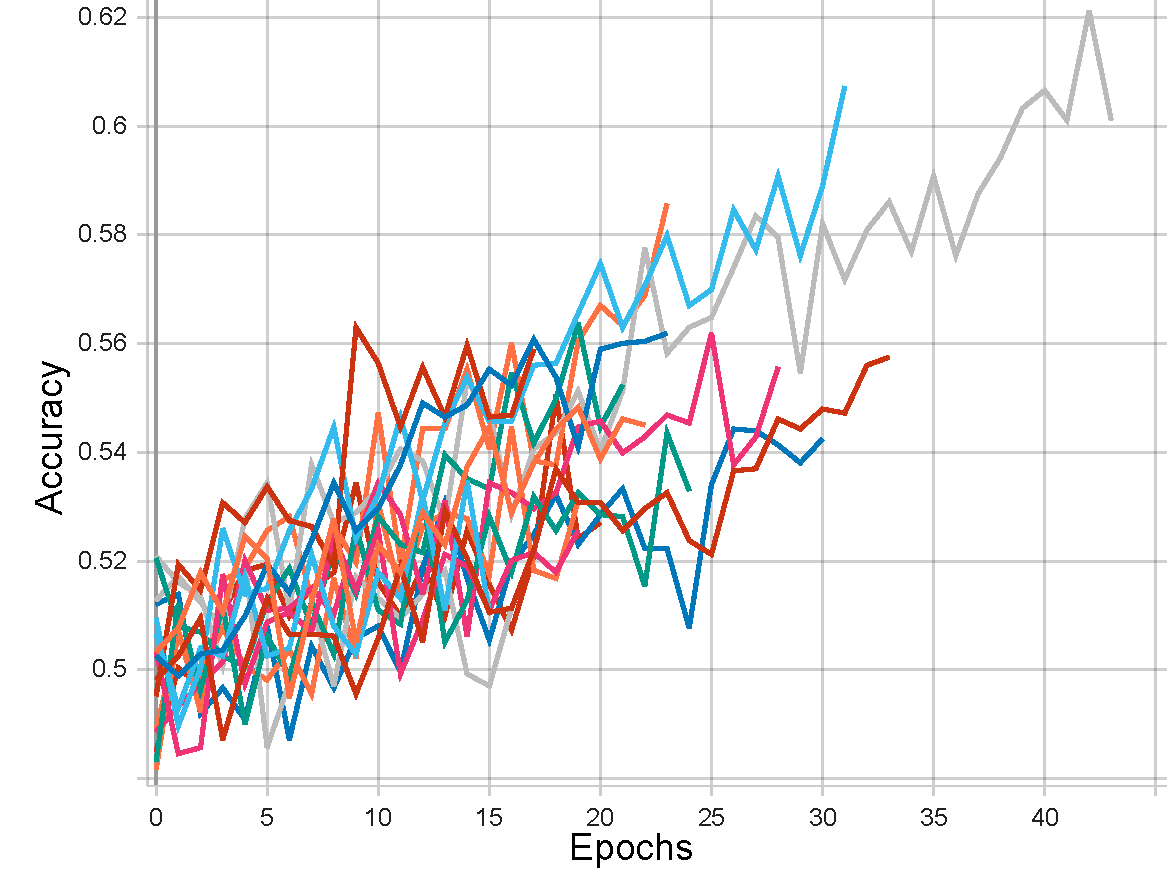
\includegraphics[width=0.95\columnwidth]{figures/results/lstm/lstm_all_acc_t.pdf}
    \caption[Training accuracies for Iteration 1]{Figure of all training accuracies of the combinations of LSTM Layers and Dense Layers in Iteration 1}
    \label{fig:iteration1_train_accuracy}
\end{figure}
\FloatBarrier

\begin{figure}[ht]
    \centering
    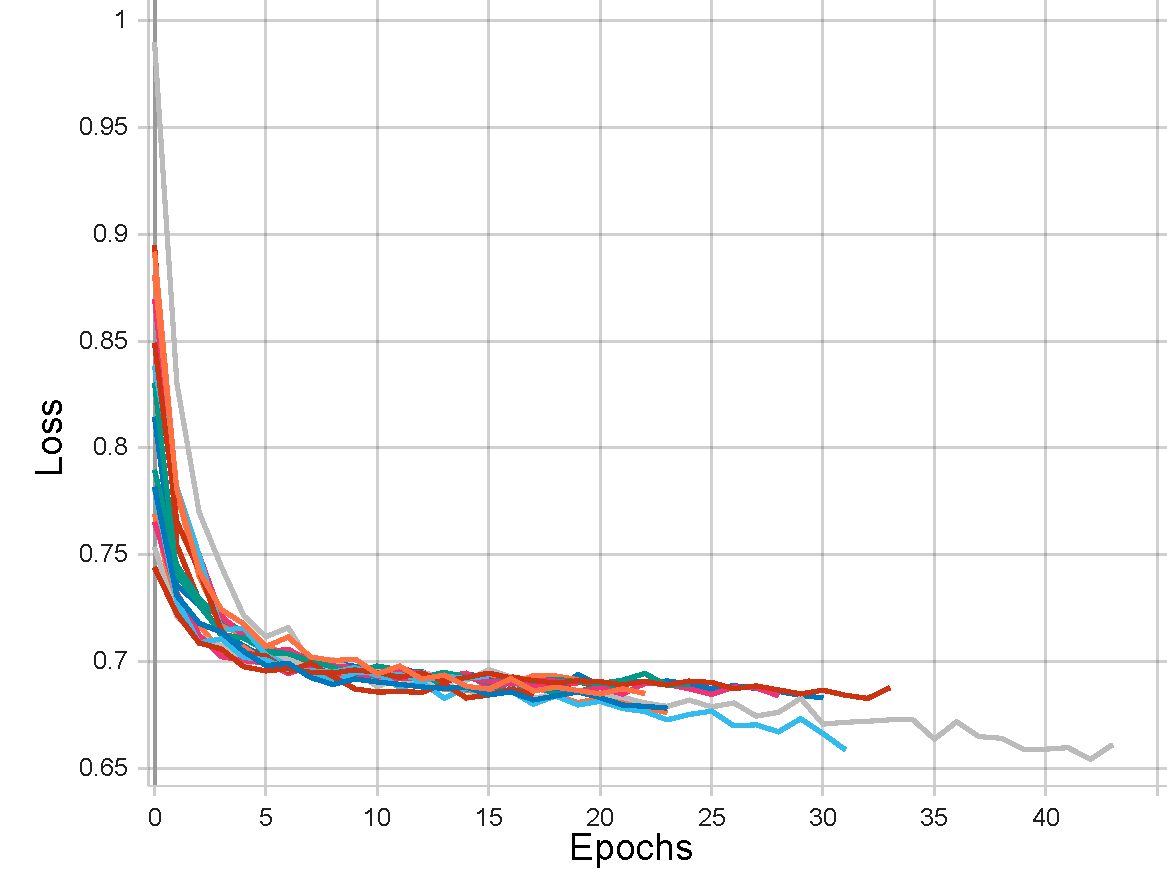
\includegraphics[width=0.95\columnwidth]{figures/results/lstm/lstm_all_loss_t.pdf}
    \caption[Training losses for Iteration 1]{Figure of all training losses of the combinations of LSTM Layers and Dense Layers in Iteration 1}
    \label{fig:iteration1_train_loss}
\end{figure}
\FloatBarrier

\subsubsection{Validation accuracies and losses}
\begin{figure}[ht]
    \centering
    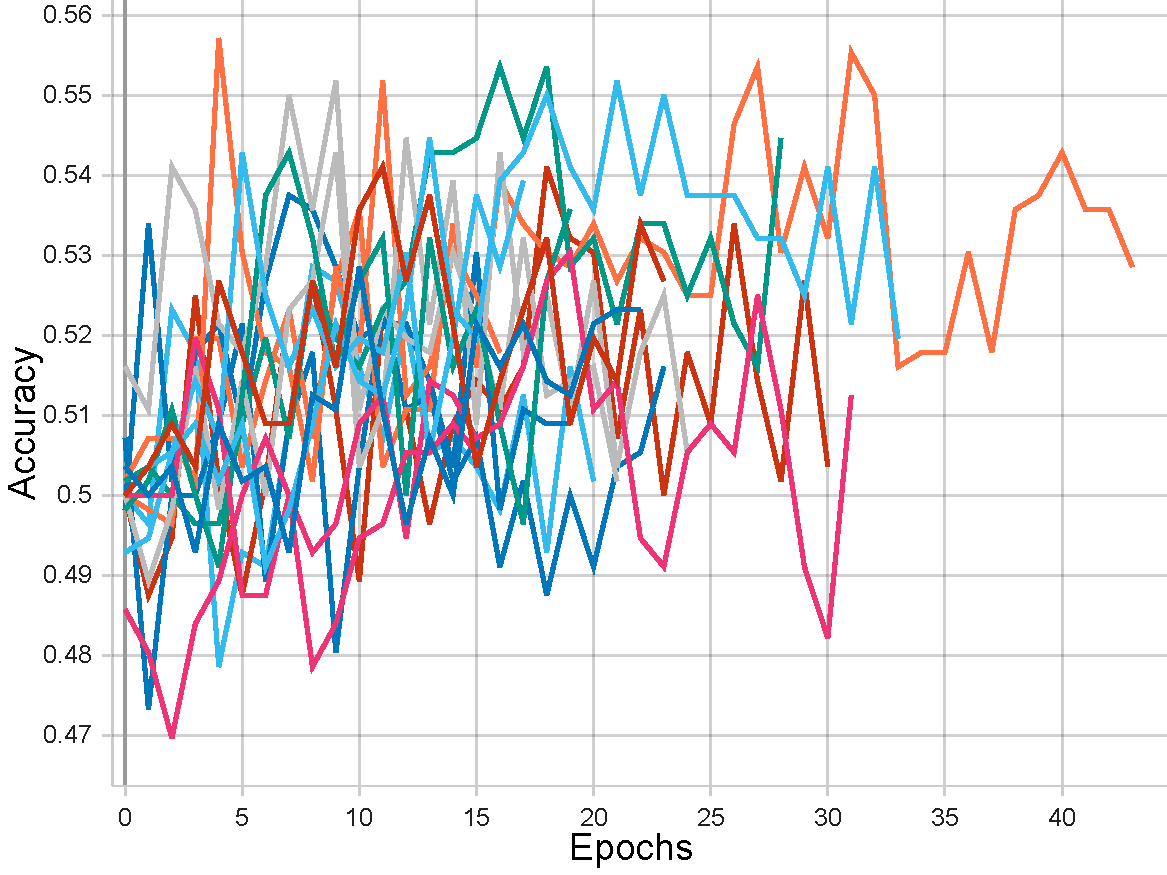
\includegraphics[width=0.95\columnwidth]{figures/results/lstm/lstm_all_acc.pdf}
    \caption[Validation accuracies for Iteration 1]{Figure of all validation accuracies of the combinations of LSTM Layers and Dense Layers in Iteration 1}
    \label{fig:iteration1_all_accuracy}
\end{figure}
\FloatBarrier

\begin{figure}[ht]
    \centering
    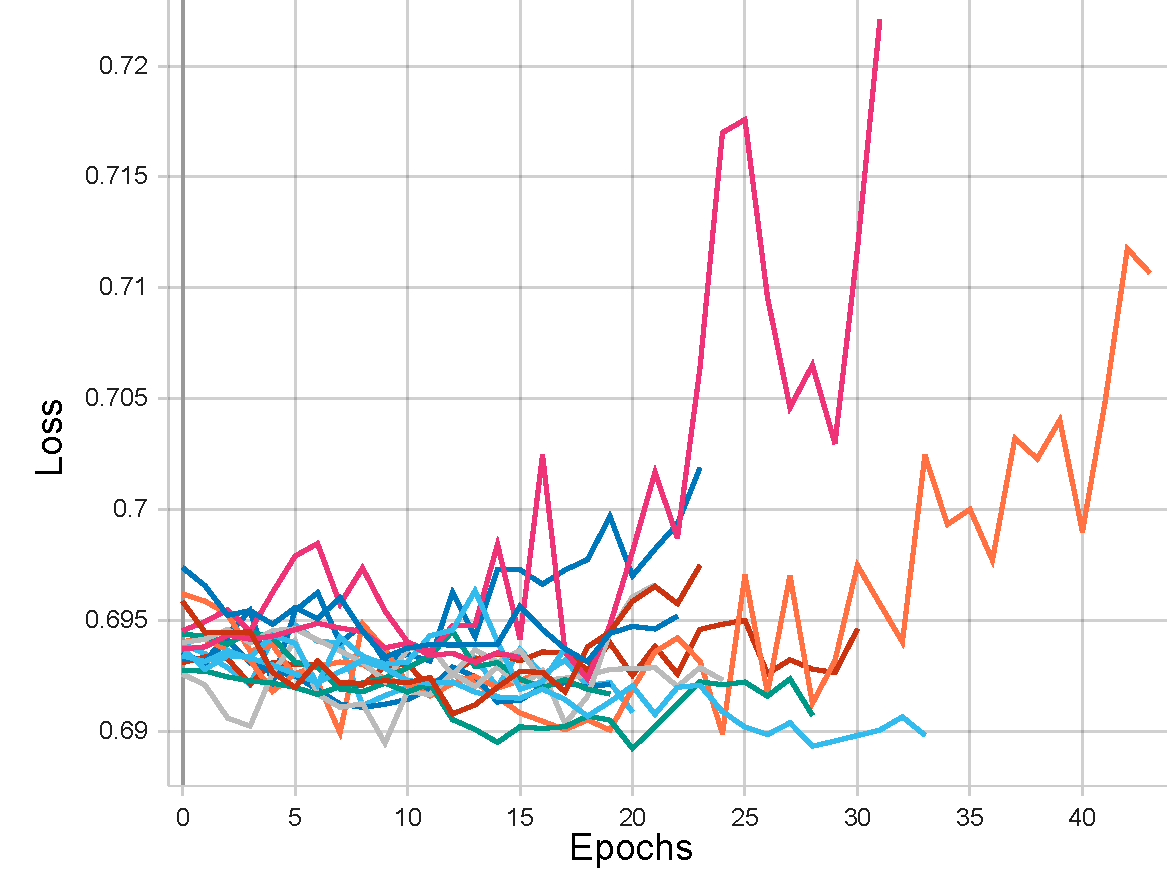
\includegraphics[width=0.95\columnwidth]{figures/results/lstm/lstm_all_loss.pdf}
    \caption[Validation losses for Iteration 1]{Figure of all validation losses of the combinations of LSTM Layers and Dense Layers in Iteration 1}
    \label{fig:iteration1_all_loss}
\end{figure}
\FloatBarrier

There are varying degrees of success with different combinations of layers; some do not improve in accuracy and others do.
The validation losses using the sparse categorical loss function as described earlier in \autoref{sec:model_fitting}
were used to help identify which models had the lowest error rate; and as an increasing validation
loss is an indicator of overfitting, it was used to filter models showing overfitting.

\subsection{Accuracies of the best result}
\begin{figure}[ht]
    \centering
    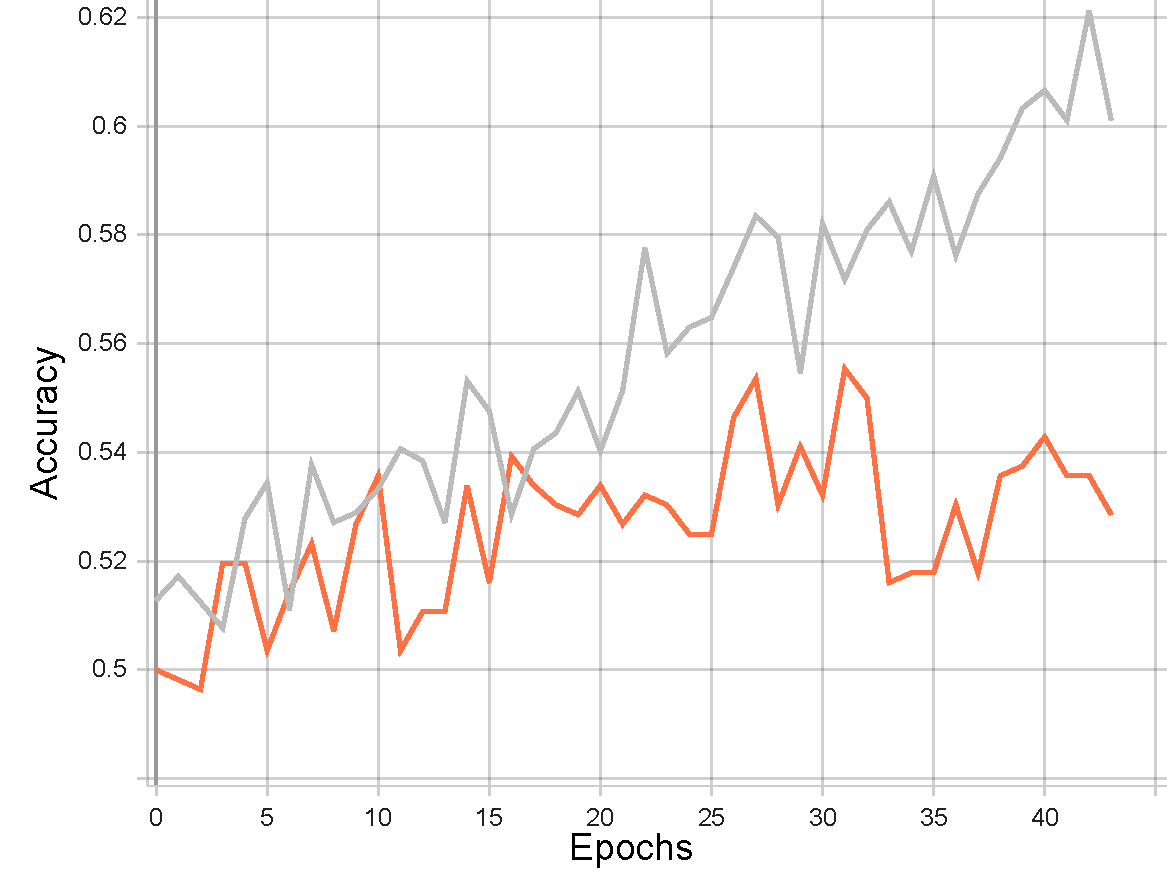
\includegraphics[width=0.95\columnwidth]{figures/results/lstm/lstm_2L64-2D32_acc.pdf}
    \caption[Best accuracy for Iteration 1]{Figure of the best accuracy of the combinations of LSTM Layers and Dense Layers in Iteration 1}
    \label{fig:iteration1_best_accuracy}
\end{figure}
\FloatBarrier

\begin{figure}[ht]
    \centering
    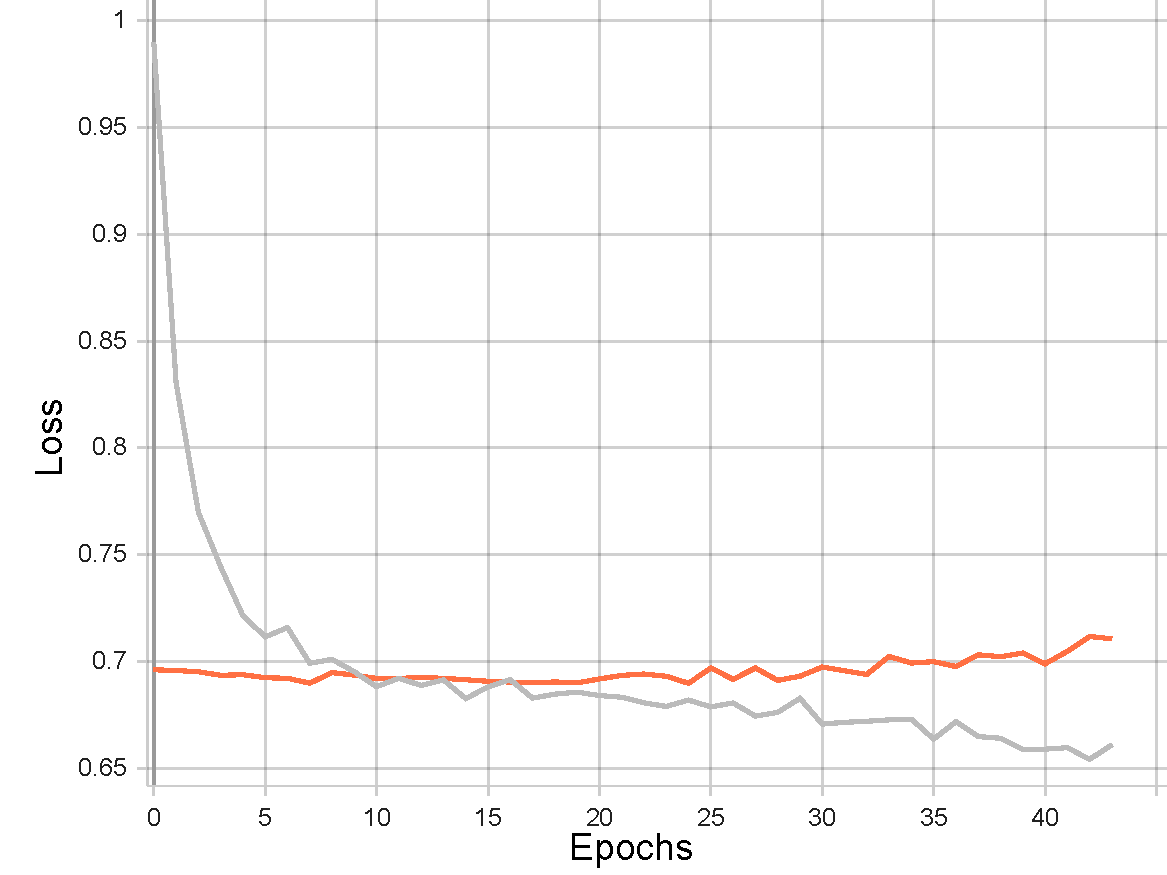
\includegraphics[width=0.95\columnwidth]{figures/results/lstm/lstm_2L64-2D32_loss.pdf}
    \caption[Best loss for Iteration 1]{Figure of the best loss of the combinations of LSTM Layers and Dense Layers in Iteration 1}
    \label{fig:iteration1_best_loss}
\end{figure}
\FloatBarrier

The best model found within this iteration was one with a two LSTM layers of size 64 followed
by the final Dense layer of size 2. The grey line represents the training set and the orange line represents
the validation set. The validation loss shows little overfitting as can be seen in
\autoref{fig:iteration1_best_loss}. At 31 epochs, the validation accuracy reaches its highest value of
55.54\% whilst the training accuracy reached above 57.18\%.
\subsection{Evaluation of iteration 1}
With a validation accuracy above 55\% it suggests that there is improvement above a random choice. It forms a good
basis for testing further AI models, specifically the CNN-LSTM hybrid model.
There are various limitations regarding iteration 1. This iteration does not test various combinations of
input features nor does it test various sequence lengths. Furthermore, there could be another number of layers or
layer sizes that is better suited to the problem, but unfortunately many have not been tested due to time constraints.

\section{Iteration 2 results}\label{iteration2_results}
As mentioned in \autoref{ssec:iteration2layers}, various combinations of Conv1D layers and Dense layers were tested,
each with various sizes. The results of all the models can be seen in \autoref{fig:iteration2_train_accuracy}
and \autoref{fig:iteration2_all_accuracy}.\\
The results of the best model can be seen in \autoref{fig:iteration2_best_accuracy}.

\subsection{Accuracies of all tests}
In the charts below, each line represents a combination of different layer types and sizes of the Dense and LSTM layers of the chart.
For both the training and validation accuracy charts, each line has a corresponding line in the loss charts with the same colour.
There are 16 lines in total for this iteration as there were 2 Conv1D layer amounts, 2 Dense layer amounts,
2 Conv1D layer sizes, and 2 Dense layer sizes in the tests.

\subsubsection{Training accuracies and losses}
\begin{figure}[ht]
    \centering
    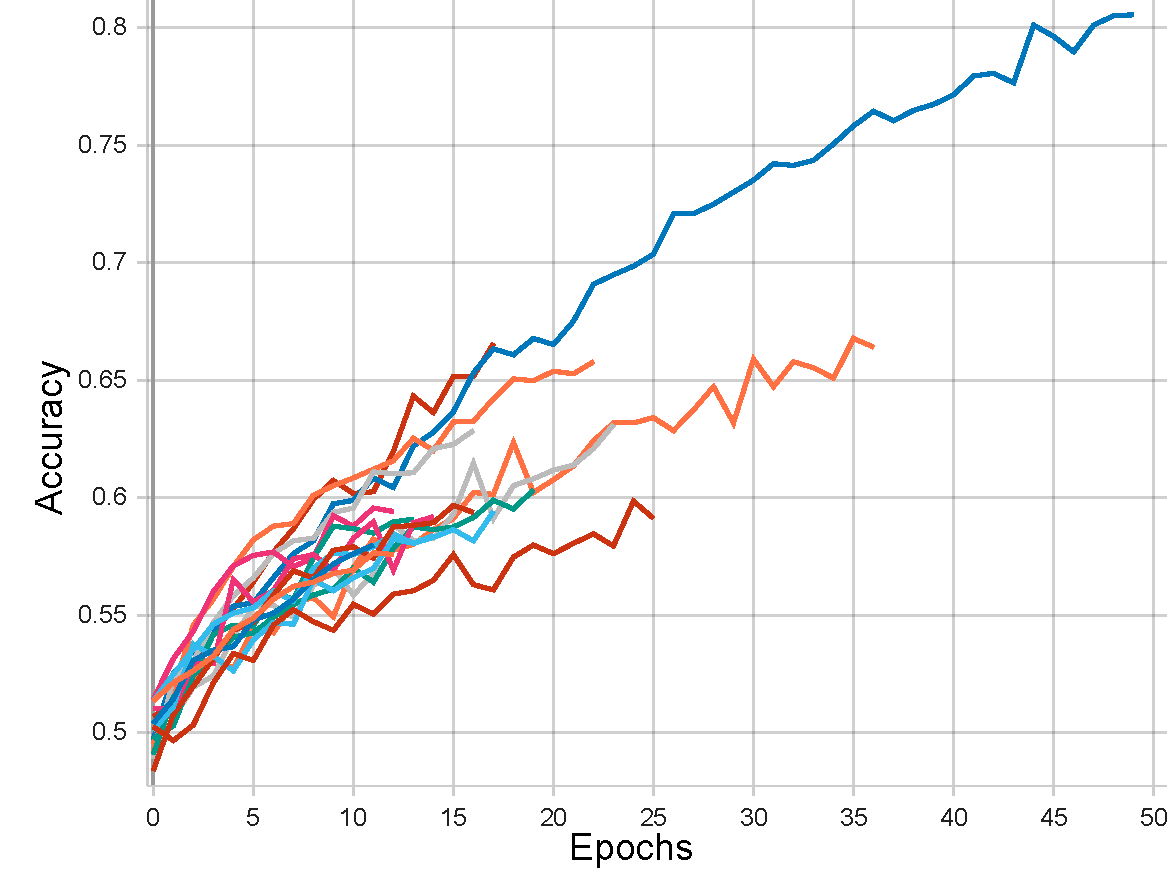
\includegraphics[width=0.95\columnwidth]{figures/results/cnn/cnn_all_acc_t.pdf}
    \caption[Training accuracies for Iteration 2]{Figure of all training accuracies of the combinations of Conv1D Layers and Dense Layers in Iteration 2}
    \label{fig:iteration2_train_accuracy}
\end{figure}
\FloatBarrier

\begin{figure}[ht]
    \centering
    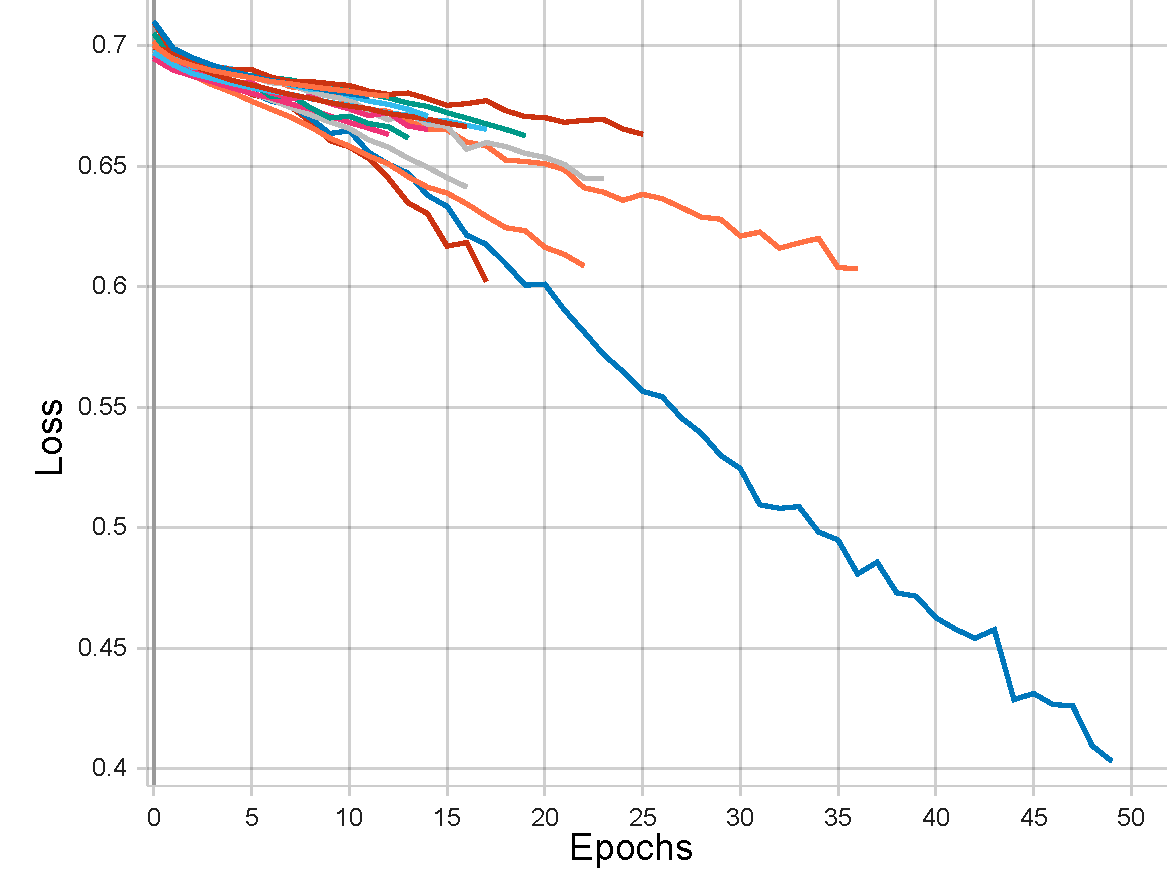
\includegraphics[width=0.95\columnwidth]{figures/results/cnn/cnn_all_loss_t.pdf}
    \caption[Training losses for Iteration 2]{Figure of all training losses of the combinations of Conv1D Layers and Dense Layers in Iteration 2}
    \label{fig:iteration2_train_loss}
\end{figure}
\FloatBarrier

\subsubsection{Validation accuracies and losses}
\begin{figure}[ht]
    \centering
    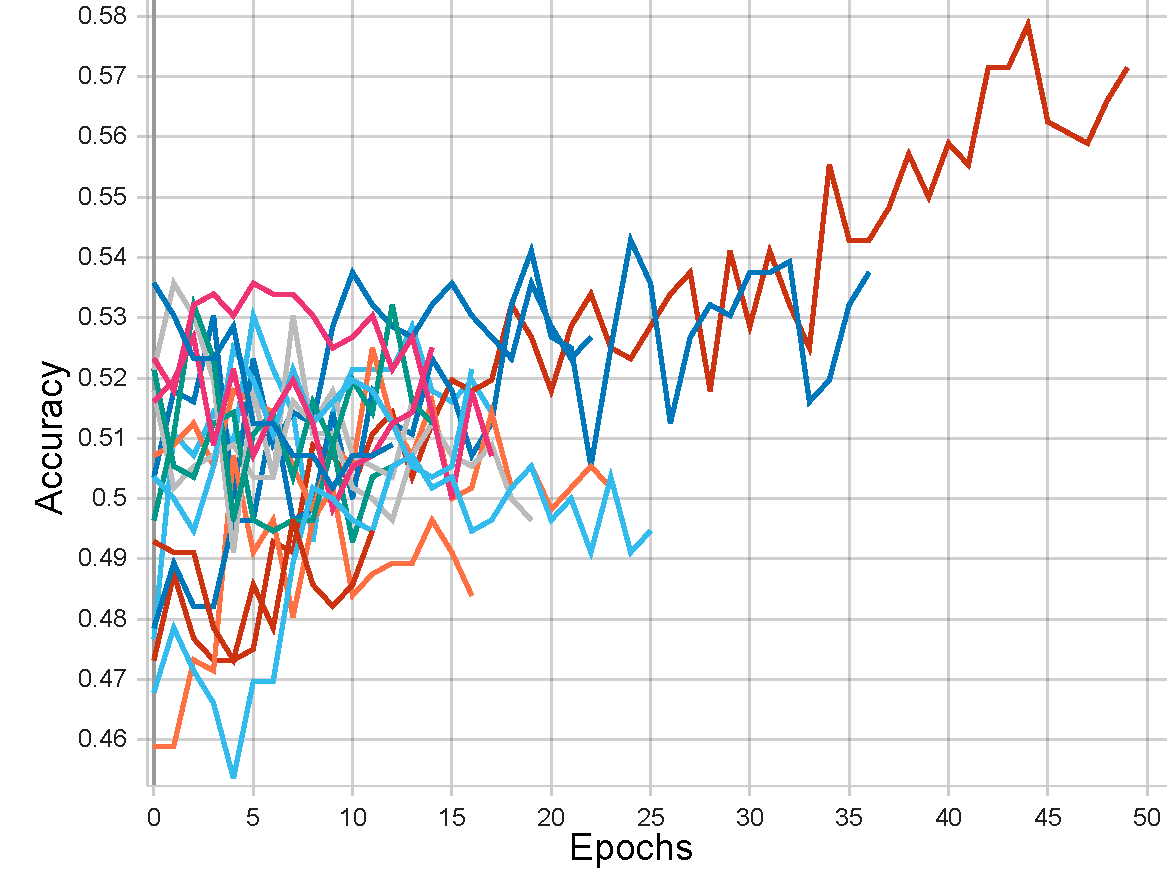
\includegraphics[width=0.95\columnwidth]{figures/results/cnn/cnn_all_acc.pdf}
    \caption[Validation accuracies for Iteration 2]{Figure of all validation accuracies of the combinations of Conv1D Layers and Dense Layers in Iteration 2}
    \label{fig:iteration2_all_accuracy}
\end{figure}
\FloatBarrier

\begin{figure}[ht]
    \centering
    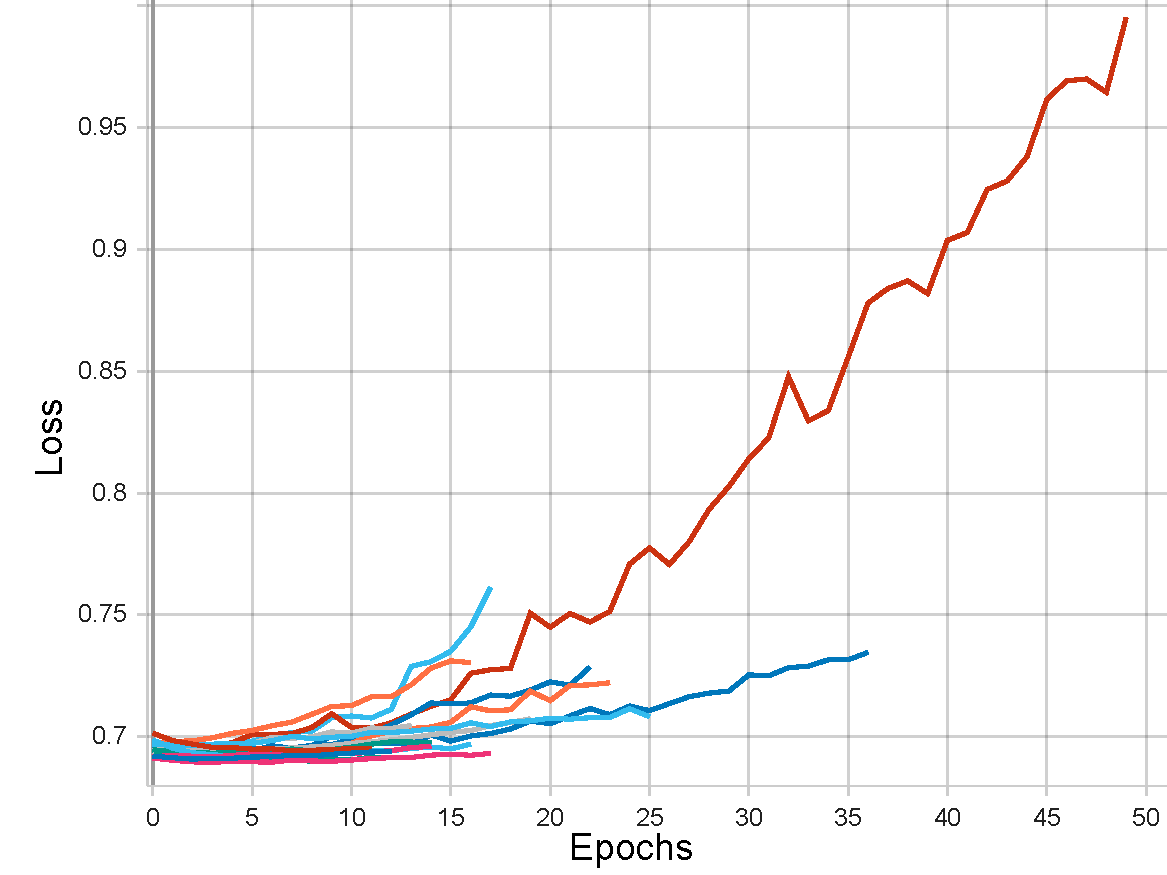
\includegraphics[width=0.95\columnwidth]{figures/results/cnn/cnn_all_loss.pdf}
    \caption[Validation losses for Iteration 2]{Figure of all validation losses of the combinations of Conv1D Layers and Dense Layers in Iteration 2}
    \label{fig:iteration2_all_loss}
\end{figure}
\FloatBarrier

There are varying degrees of success with different combinations of layers; some do not improve in accuracy and others do.
The validation losses using the sparse categorical loss function as described earlier in \autoref{sec:model_fitting}
were used to help identify which models had the lowest error rate; and as an increasing validation
loss is an indicator of overfitting, it was used to filter models showing overfitting.

\subsection{Accuracies of the best result}
\begin{figure}[ht]
    \centering
    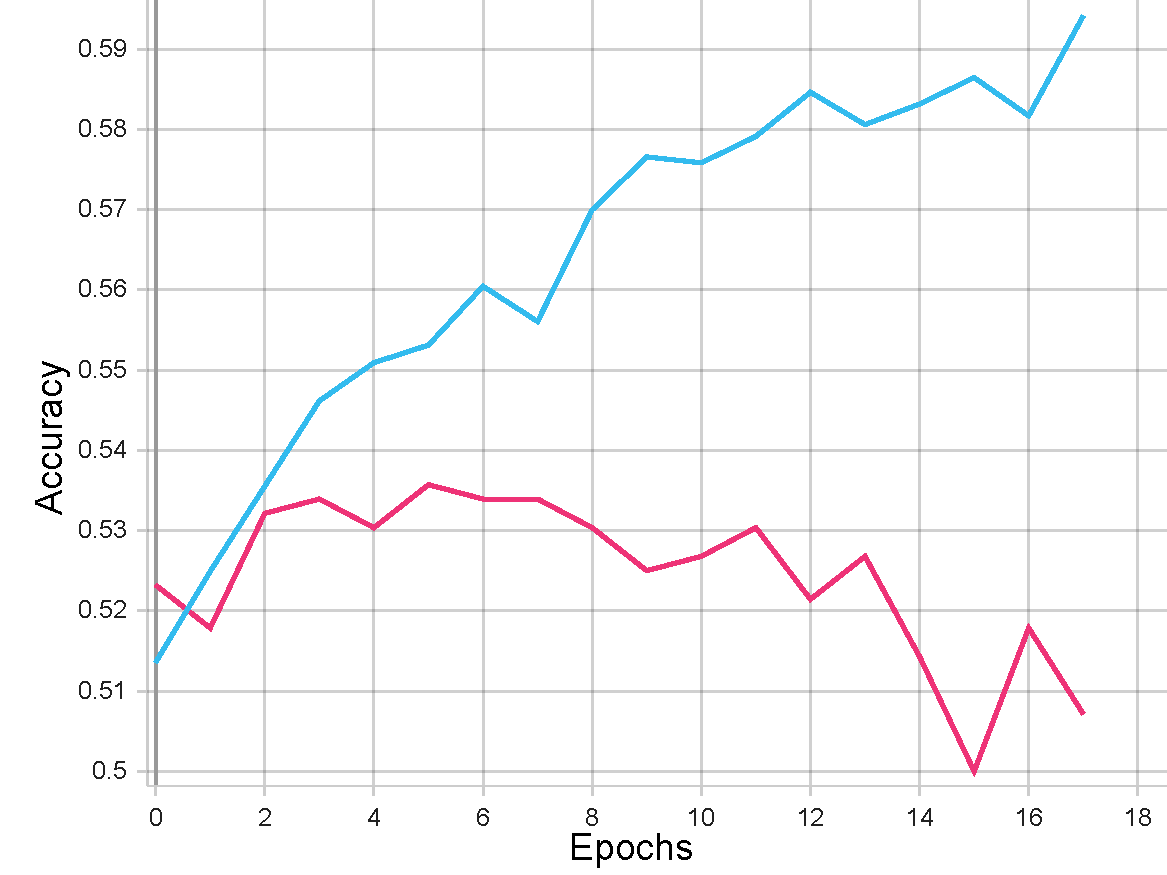
\includegraphics[width=0.95\columnwidth]{figures/results/cnn/cnn_1C32-1D64_acc.pdf}
    \caption[Best accuracy for Iteration 2]{Figure of the best accuracy of the combinations of Conv1D Layers and Dense Layers in Iteration 2}
    \label{fig:iteration2_best_accuracy}
\end{figure}
\FloatBarrier

\begin{figure}[ht]
    \centering
    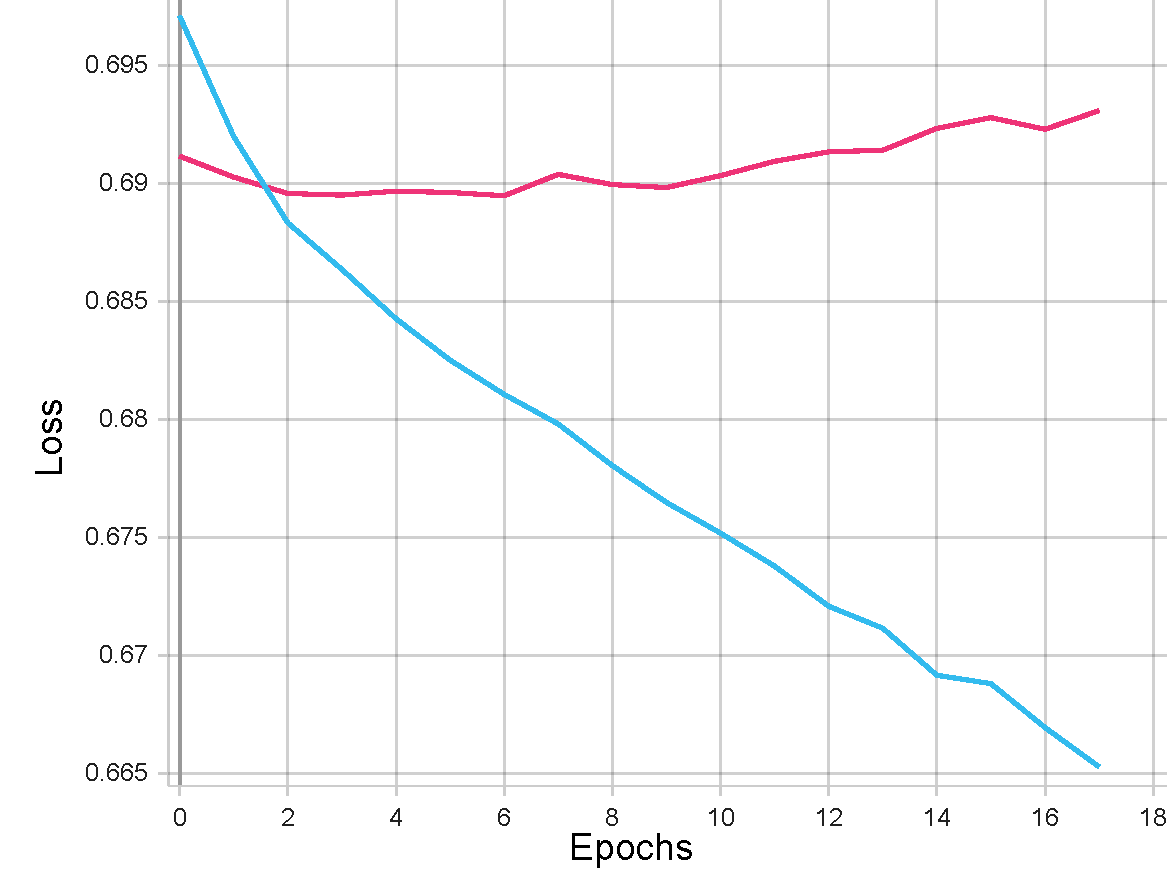
\includegraphics[width=0.95\columnwidth]{figures/results/cnn/cnn_1C32-1D64_loss.pdf}
    \caption[Best loss for Iteration 2]{Figure of the best loss of the combinations of Conv1D Layers and Dense Layers in Iteration 2}
    \label{fig:iteration2_best_loss}
\end{figure}
\FloatBarrier

The best model found within this iteration was one with a one CNN layer of size 32 followed
by the final Dense layer of size 2. The blue line represents the training set and the pink line represents
the validation set. The validation loss shows little overfitting as can be seen in
\autoref{fig:iteration2_best_loss}. At 5 epochs, the validation accuracy reaches its highest value of
53.57\% whilst the training accuracy reached above 55.31\%.
\subsection{Evaluation of iteration 2}
With a validation accuracy above 53\% it suggests that there is only minimal improvement above a random choice. It forms a good
basis for testing further AI models, specifically the CNN-LSTM hybrid model.
There are various limitations regarding iteration 2. This iteration does not test various combinations of
input features nor does it test various sequence lengths. Furthermore, there could be another number of layers or
layer sizes that is better suited to the problem, but unfortunately many have not been tested due to time constraints.

\section{Iteration 3 results}\label{iteration3_results}
As mentioned in \autoref{ssec:iteration3layers}, various combinations of Conv1D layers, LSTM layers and Dense layers were tested,
each with various sizes. The results of all the models can be seen in \autoref{fig:iteration3_train_accuracy}
and \autoref{fig:iteration3_all_accuracy}.\\
The results of the best model can be seen in \autoref{fig:iteration3_best_accuracy}.

\subsection{Accuracies of all tests}
In the charts below, each line represents a combination of different layer types and sizes of the Conv1D, LSTM and Dense layers.
For both the training and validation accuracy charts, each line has a corresponding line in the loss charts with the same colour.
There are 64 lines in total for this iteration as there were 2 Conv1D layer amounts, 2 LSTM layer amounts, 2 Dense layer amounts,
as well as 2 Conv1D layer sizes, 2 LSTM layer sizes and 2 Dense layer sizes in the tests.

\subsubsection{Training accuracies and losses}
\begin{figure}[ht]
    \centering
    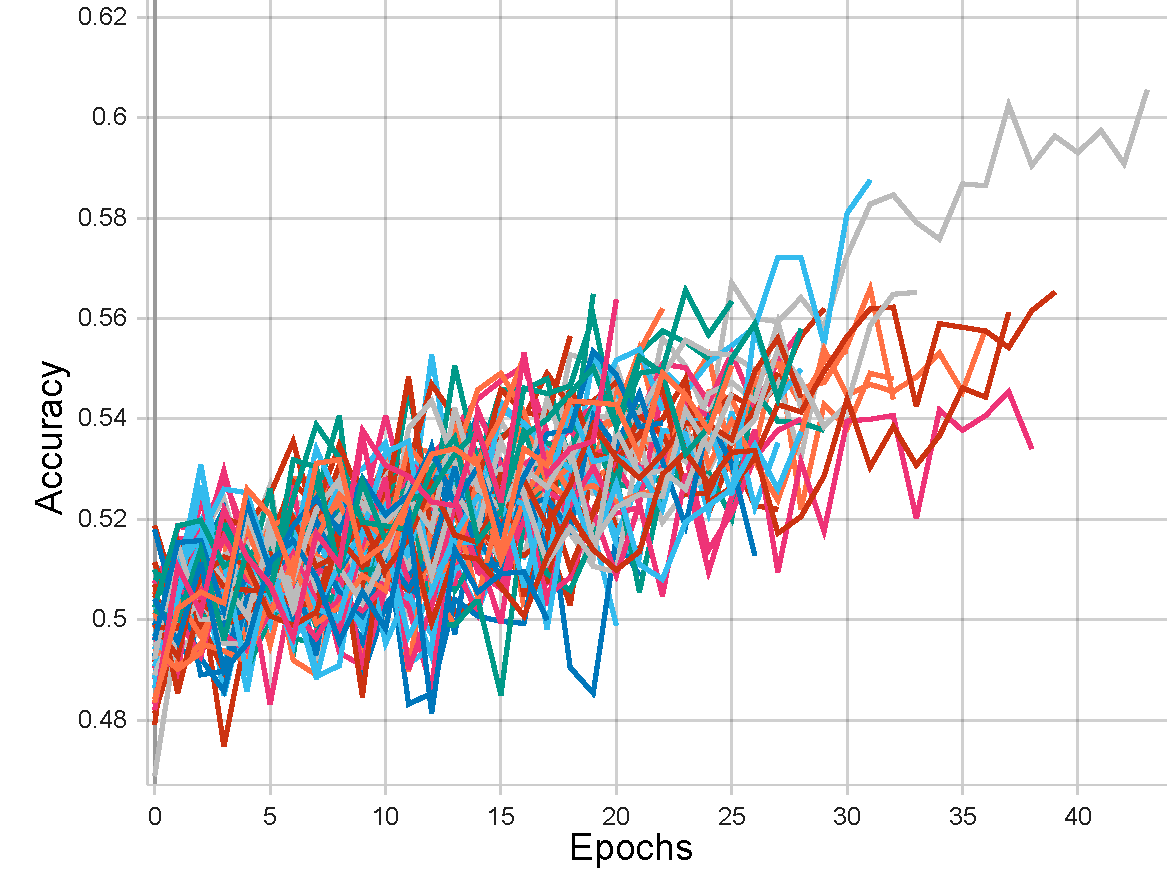
\includegraphics[width=0.95\columnwidth]{figures/results/cnnlstm/cnnlstm_all_acc_t.pdf}
    \caption[Training accuracies for Iteration 3]{Figure of all training accuracies of the combinations of Conv1D, LSTM and Dense Layers in Iteration 3}
    \label{fig:iteration3_train_accuracy}
\end{figure}
\FloatBarrier

\begin{figure}[ht]
    \centering
    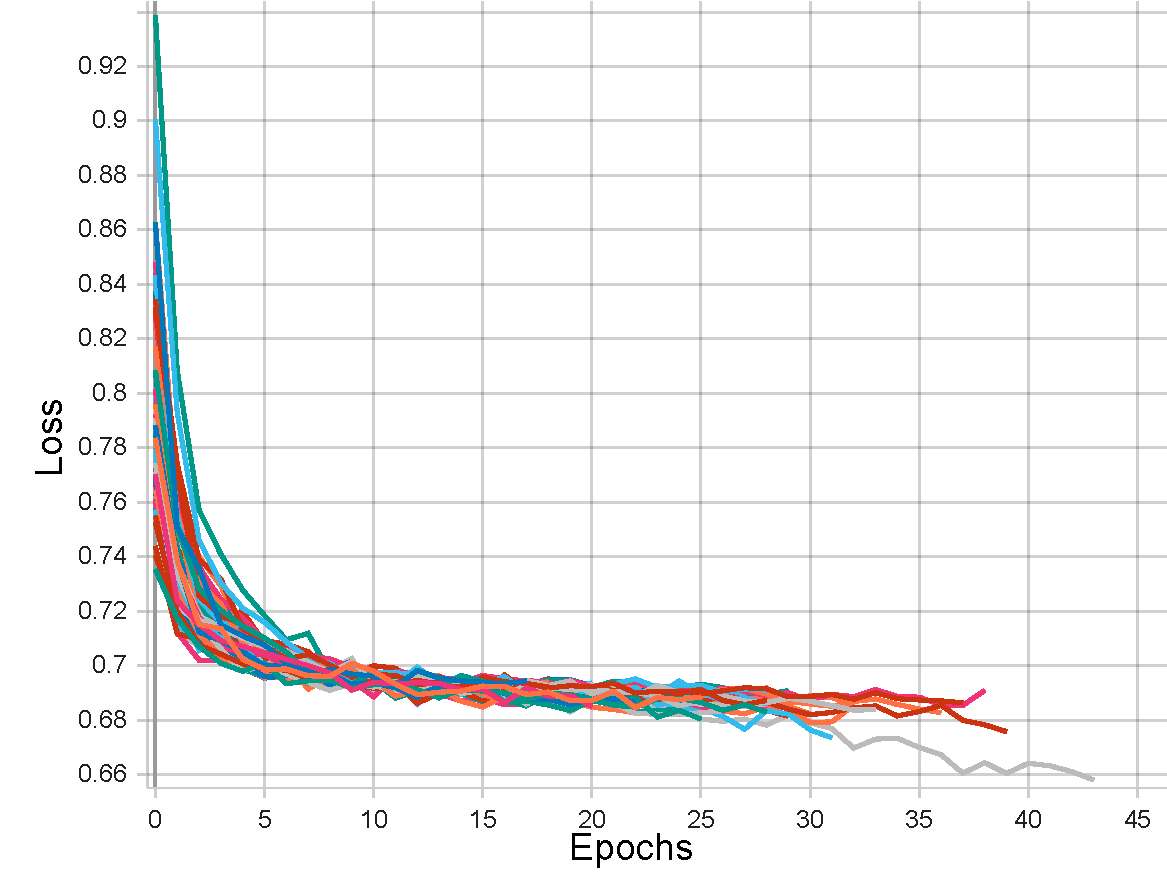
\includegraphics[width=0.95\columnwidth]{figures/results/cnnlstm/cnnlstm_all_loss_t.pdf}
    \caption[Training losses for Iteration 3]{Figure of all training losses of the combinations of Conv1D, LSTM and Dense Layers in Iteration 3}
    \label{fig:iteration3_train_loss}
\end{figure}
\FloatBarrier

\subsubsection{Validation accuracies and losses}
\begin{figure}[ht]
    \centering
    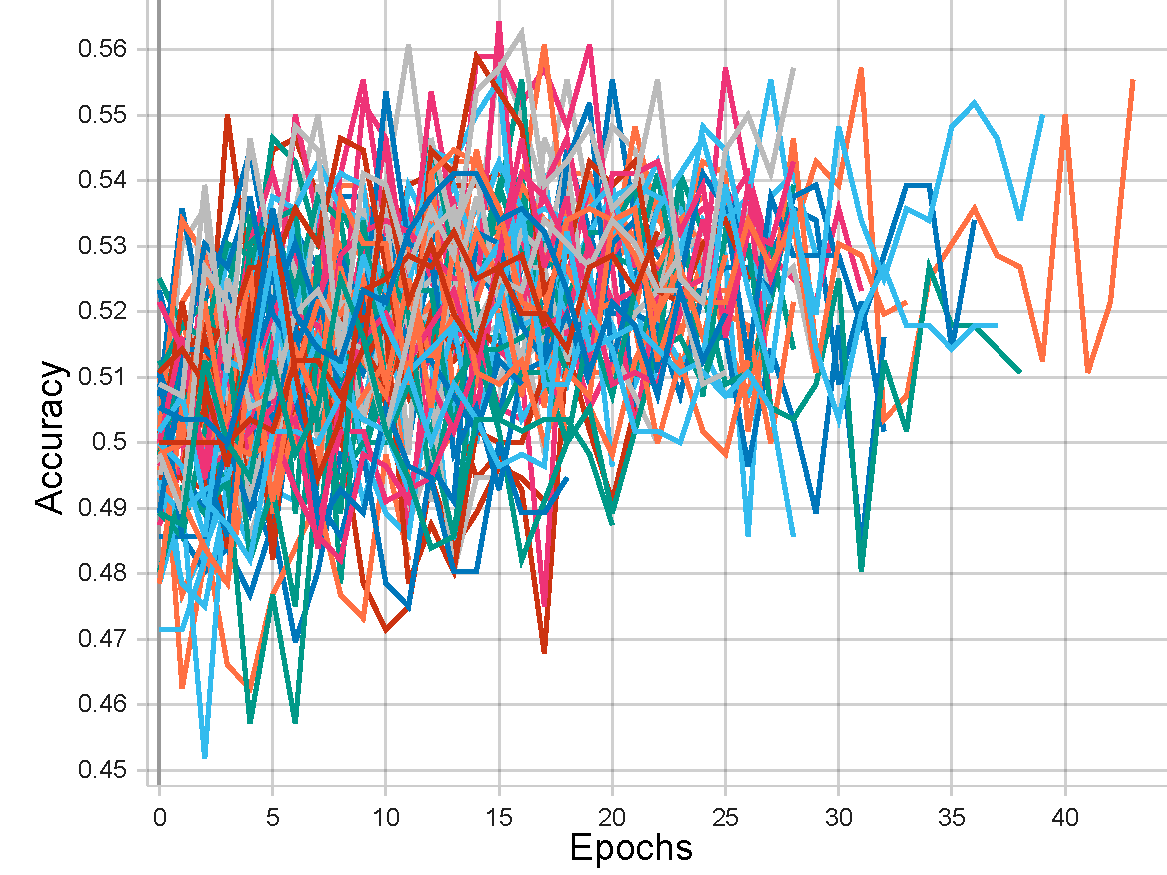
\includegraphics[width=0.95\columnwidth]{figures/results/cnnlstm/cnnlstm_all_acc.pdf}
    \caption[Validation accuracies for Iteration 3]{Figure of all validation accuracies of the combinations of Conv1D, LSTM and Dense Layers in Iteration 3}
    \label{fig:iteration3_all_accuracy}
\end{figure}
\FloatBarrier

\begin{figure}[ht]
    \centering
    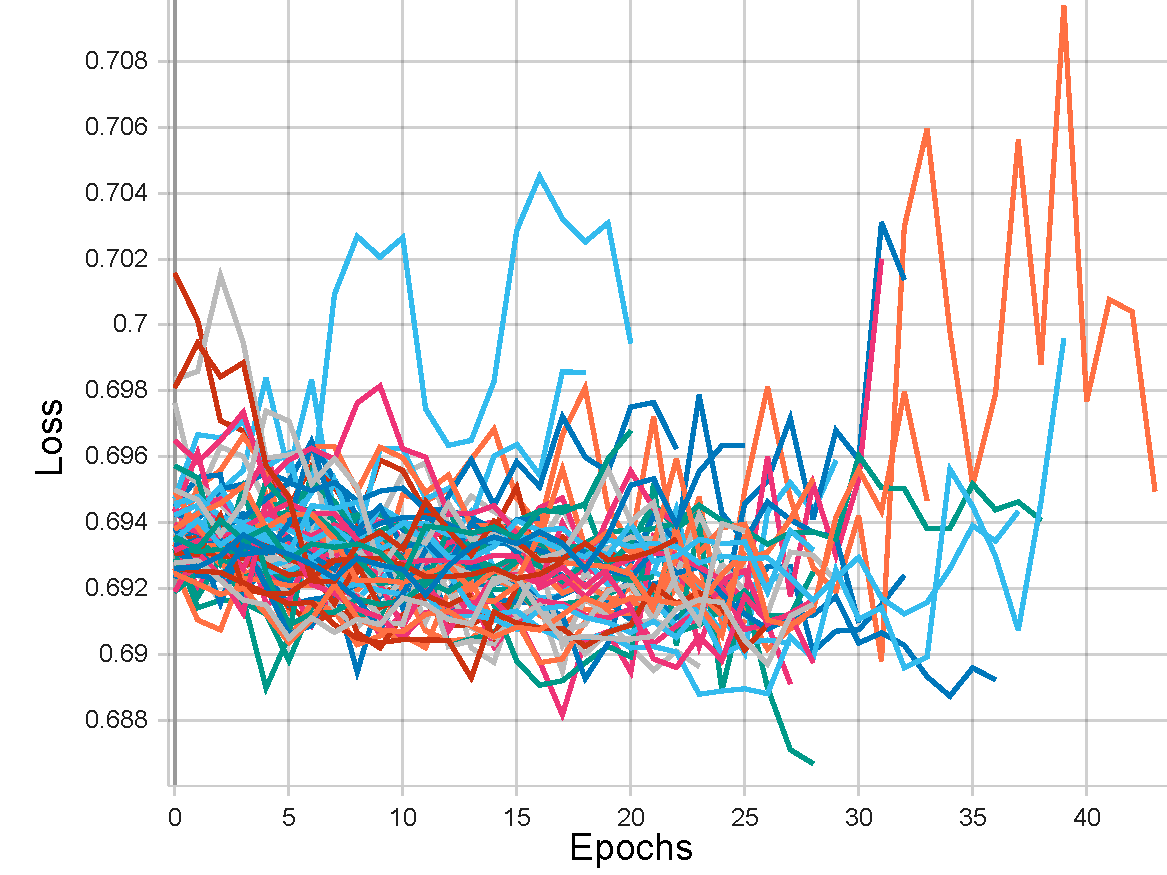
\includegraphics[width=0.95\columnwidth]{figures/results/cnnlstm/cnnlstm_all_loss.pdf}
    \caption[Validation losses for Iteration 3]{Figure of all validation losses of the combinations of Conv1D, LSTM and Dense Layers in Iteration 3}
    \label{fig:iteration3_all_loss}
\end{figure}
\FloatBarrier

There are varying degrees of success with different combinations of layers; some do not improve in accuracy and others do.
The validation losses using the sparse categorical loss function as described earlier in \autoref{sec:model_fitting}
were used to help identify which models had the lowest error rate; and as an increasing validation
loss is an indicator of overfitting, it was used to filter models showing overfitting.

\subsection{Accuracies of the best result}
\begin{figure}[ht]
    \centering
    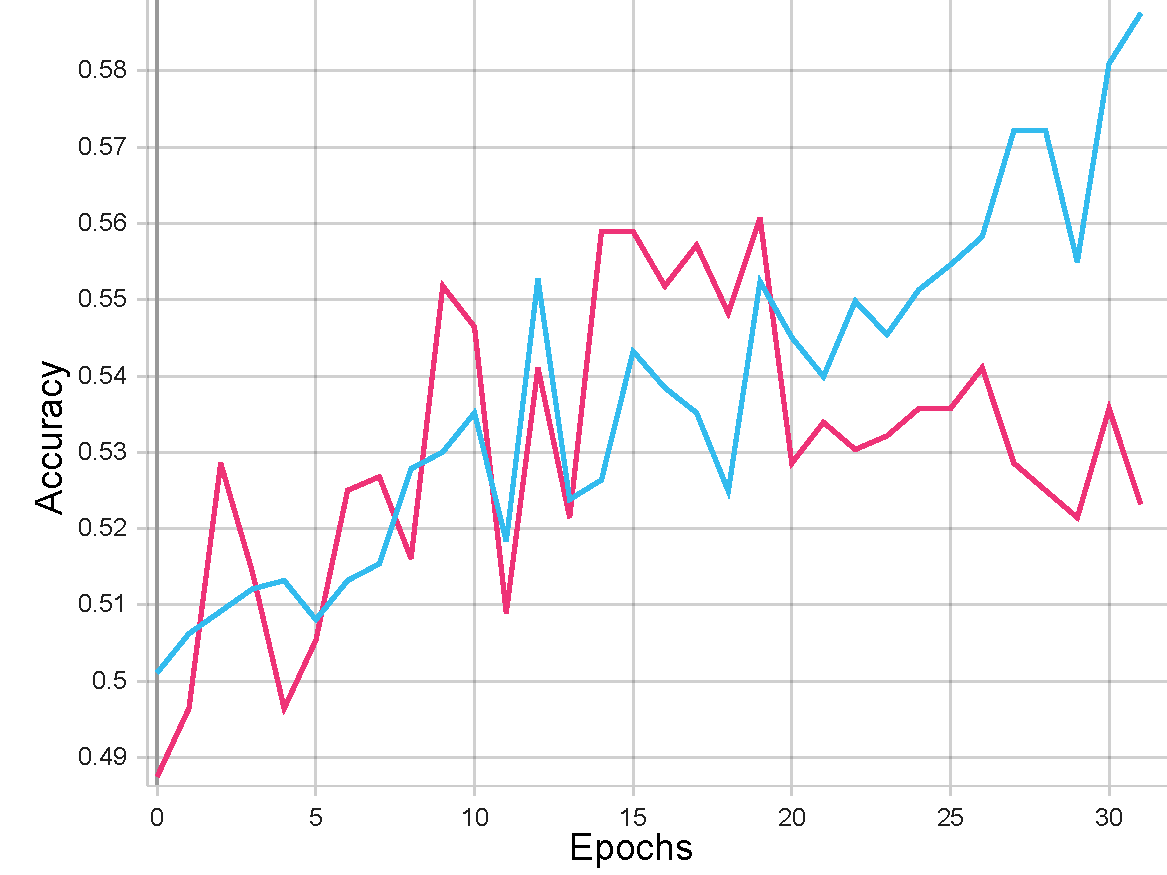
\includegraphics[width=0.95\columnwidth]{figures/results/cnnlstm/cnnlstm_2C32-1L16-2D64_acc.pdf}
    \caption[Best accuracy for Iteration 3]{Figure of the best accuracy of the combinations of Conv1D, LSTM and Dense Layers in Iteration 3}
    \label{fig:iteration3_best_accuracy}
\end{figure}
\FloatBarrier

\begin{figure}[ht]
    \centering
    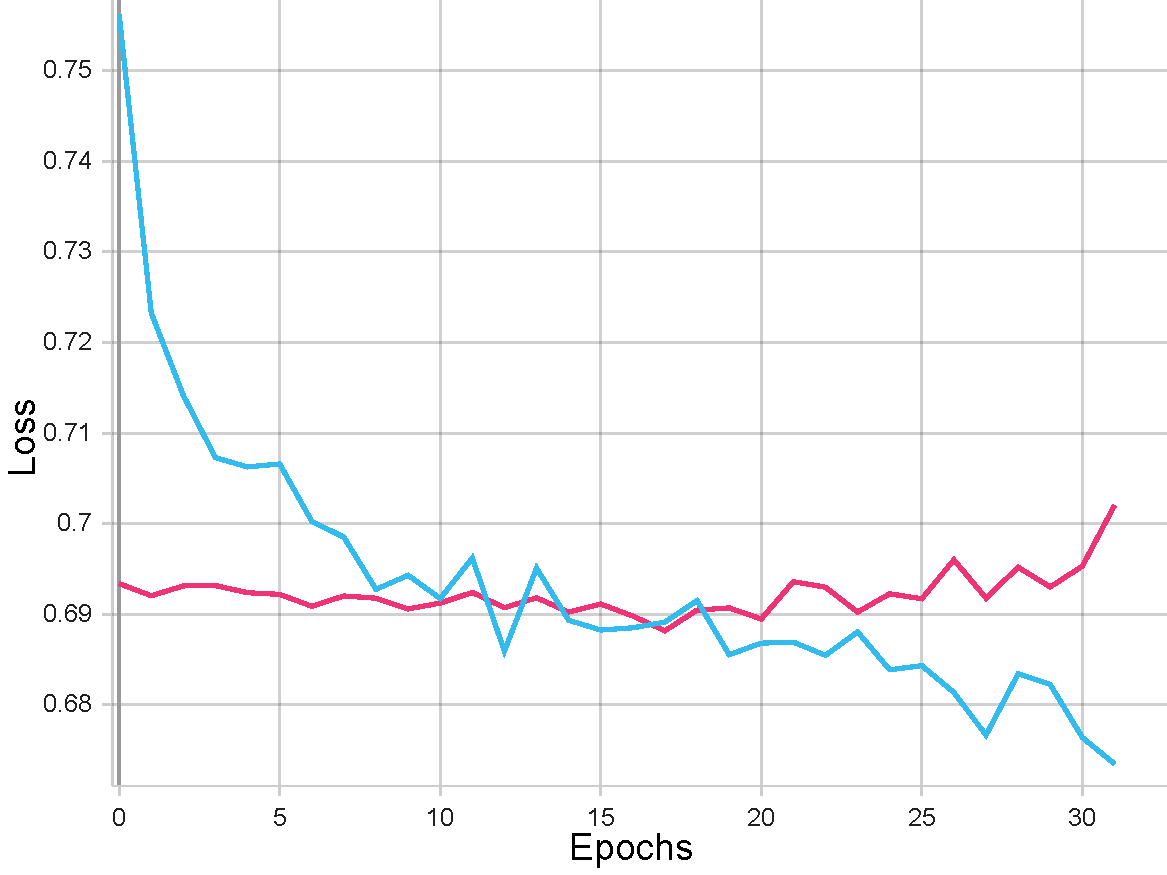
\includegraphics[width=0.95\columnwidth]{figures/results/cnnlstm/cnnlstm_2C32-1L16-2D64_loss.pdf}
    \caption[Best loss for Iteration 3]{Figure of the best loss of the combinations of Conv1D, LSTM and Dense Layers in Iteration 3}
    \label{fig:iteration3_best_loss}
\end{figure}
\FloatBarrier

The best model found within this iteration was one with a two Conv1D layers of size 32 followed by 1 LSTM layer
of size 16, and a Dense layer of size 64 followed by a final Dense layer of size 2.
The blue line represents the training set and the pink line represents
the validation set. The validation loss shows little overfitting as can be seen in
\autoref{fig:iteration3_best_loss}. At 19 epochs, the validation accuracy reaches its highest value of
56.07\% whilst the training accuracy reached 55.24\%. The validation accuracy being somewhat greater than the
training accuracy can be explained by the dropout layers within the model that can affect the results of the training
set but does not affect the validation set.

\subsection{Evaluation of iteration 3}
With a validation accuracy above 56.07\%, it is currently the best model when compared to the previous iterations.
This suggests there is a significant advantage compared to randomly guessing the next trading day's direction.
Furthermore, this aligns with the studies analysed in the literature review. However, this iteration alone cannot be
used to answer the research questions as it does not test different sequence lengths or combinations of input features.
Additionally, there could be a different number of layers or sizes of layers that perform better but unfortunately could
not be tested due to time constraints.

\section{Iteration 4 results}\label{iteration4_results}
As mentioned in \autoref{ssec:iteration4_ai_model}, a concatenated model of the best models of the previous 
three iterations were combined in parallel. The results of this model can be seen in
\autoref{fig:iteration4_accuracy}.

\subsection{Accuracies of iteration 4 model}

\begin{figure}[ht]
    \centering
    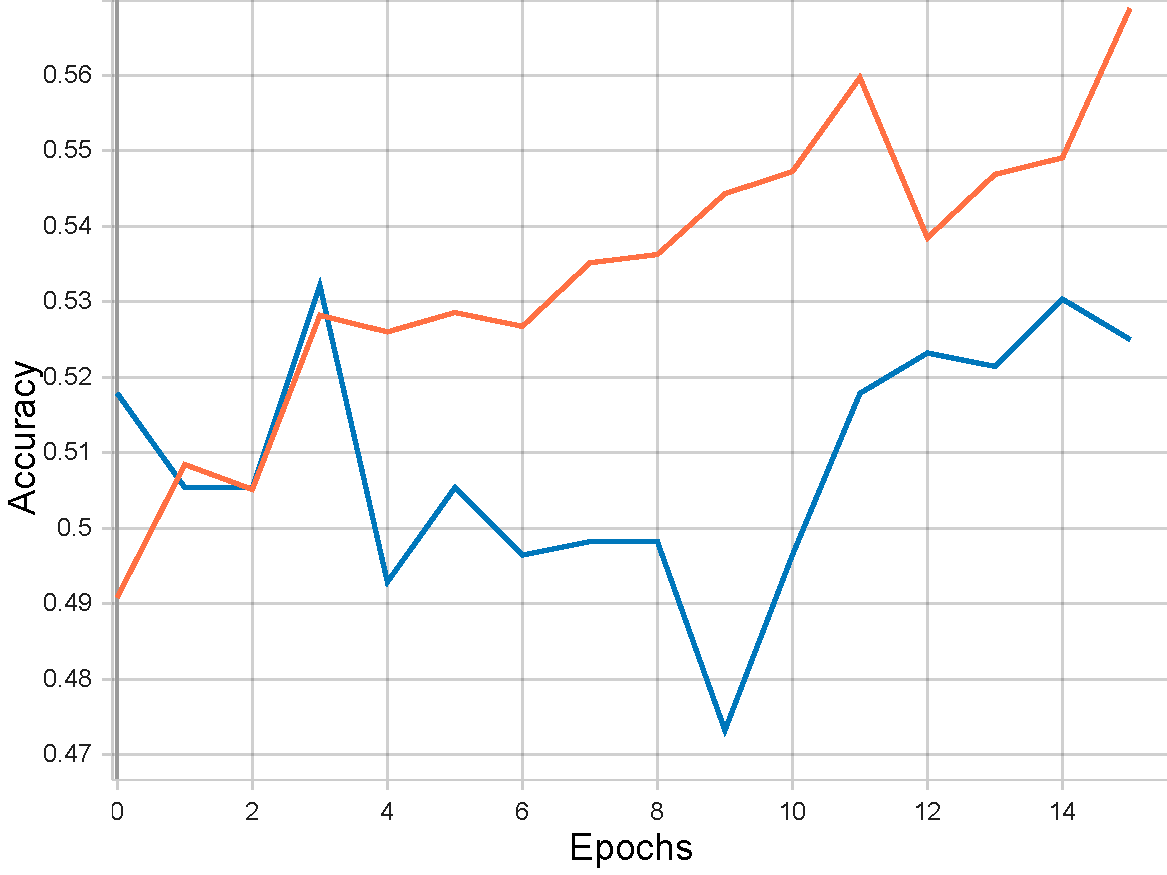
\includegraphics[width=0.95\columnwidth]{figures/results/concat/concat_acc.pdf}
    \caption[Accuracies for Iteration 4]{Figure of all training and validation accuracies in Iteration 4}
    \label{fig:iteration4_accuracy}
\end{figure}
\FloatBarrier

\begin{figure}[ht]
    \centering
    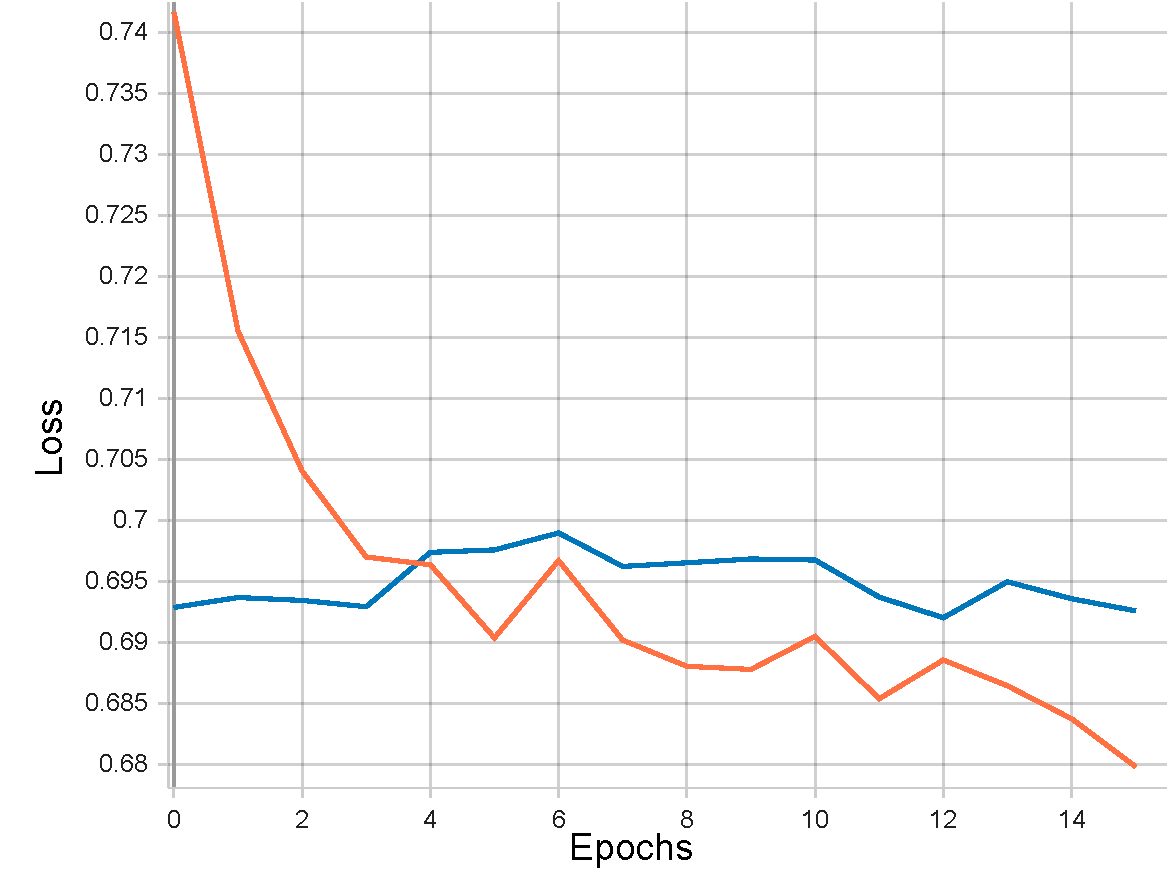
\includegraphics[width=0.95\columnwidth]{figures/results/concat/concat_loss.pdf}
    \caption[Losses for Iteration 4]{Figure of all training and validation losses in Iteration 4}
    \label{fig:iteration4_loss}
\end{figure}
\FloatBarrier

The orange line represents the training set and the blue line represents
the validation set. The validation loss shows little overfitting as can be seen in
\autoref{fig:iteration4_loss} as the loss does not significantly increase. At 3 epochs,
the validation accuracy reaches its highest value of 53.21\% whilst the training accuracy reached 52.82\%. The validation accuracy being somewhat greater than the
training accuracy can be explained by the dropout layers within the model that can affect the results of the training
set but does not affect the validation set.

\subsection{Evaluation of iteration 4}
With a validation accuracy above 53\%, there is only a minimal improvement above a random guess of the direction
of the next trading day. This model was included to test between a sequential hybrid model as seen in Iteration 3
and this parallel hybrid approach. However, this model does not offer any advantage over the CNN-LSTM sequential
model alone; due to this, no further tests will be utilised with this model.

\section{Iteration 5 results}\label{iteration5_results}
This iteration primarily used a similar model to that in Iteration 3, however with varied input features
and varied sequence lengths. There are various results that come from this model from identifying the
best amount of historic data to identifying the most important inputs.

\subsection{Accuracies of all tests}

For each of the tests in Iteration 5, the charts contain 15 lines representing the different combinations
of input features as mentioned in \autoref{ssec:iteration5_input_features}. Each line in the accuracy chart
has a corresponding line in the loss chart with the same colour. Each line in the training charts has a 
corresponding line in the validation charts with a different colour.\\
\\
The best values of the validation accuracies of each model at any epoch are shown in
\autoref{ssec:iteration5_best_val_acc}.

\subsubsection{Two days of historic data accuracies and losses}
\textbf{Training accuracies and losses}
\begin{figure}[ht]
    \centering
    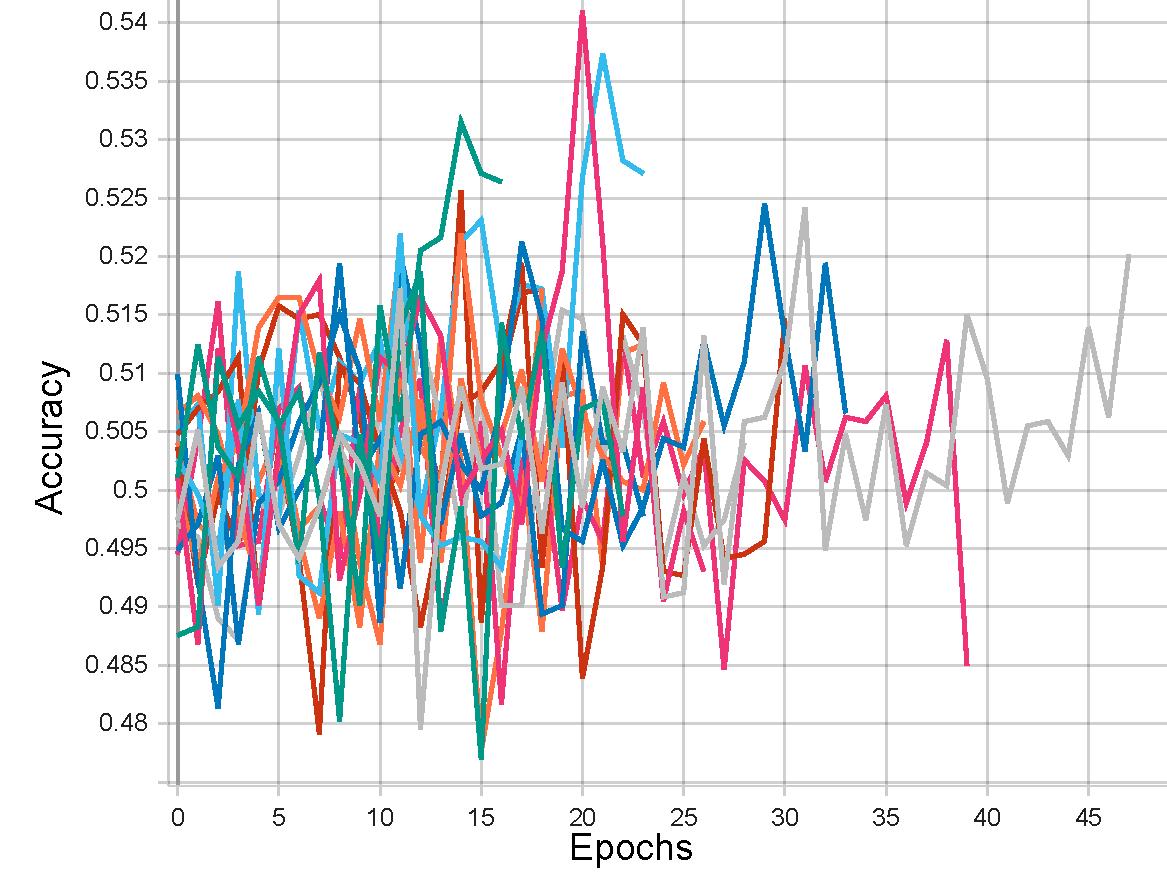
\includegraphics[width=0.575\columnwidth]{figures/results/final/two_days_acc_t.pdf}
    \caption[Training accuracies for Iteration 5 with two days of historic data]{Figure of all training accuracies with two days of historic data in Iteration 5}
    \label{fig:iteration5_two_days_train_accuracy}
\end{figure}
\FloatBarrier

\begin{figure}[ht]
    \centering
    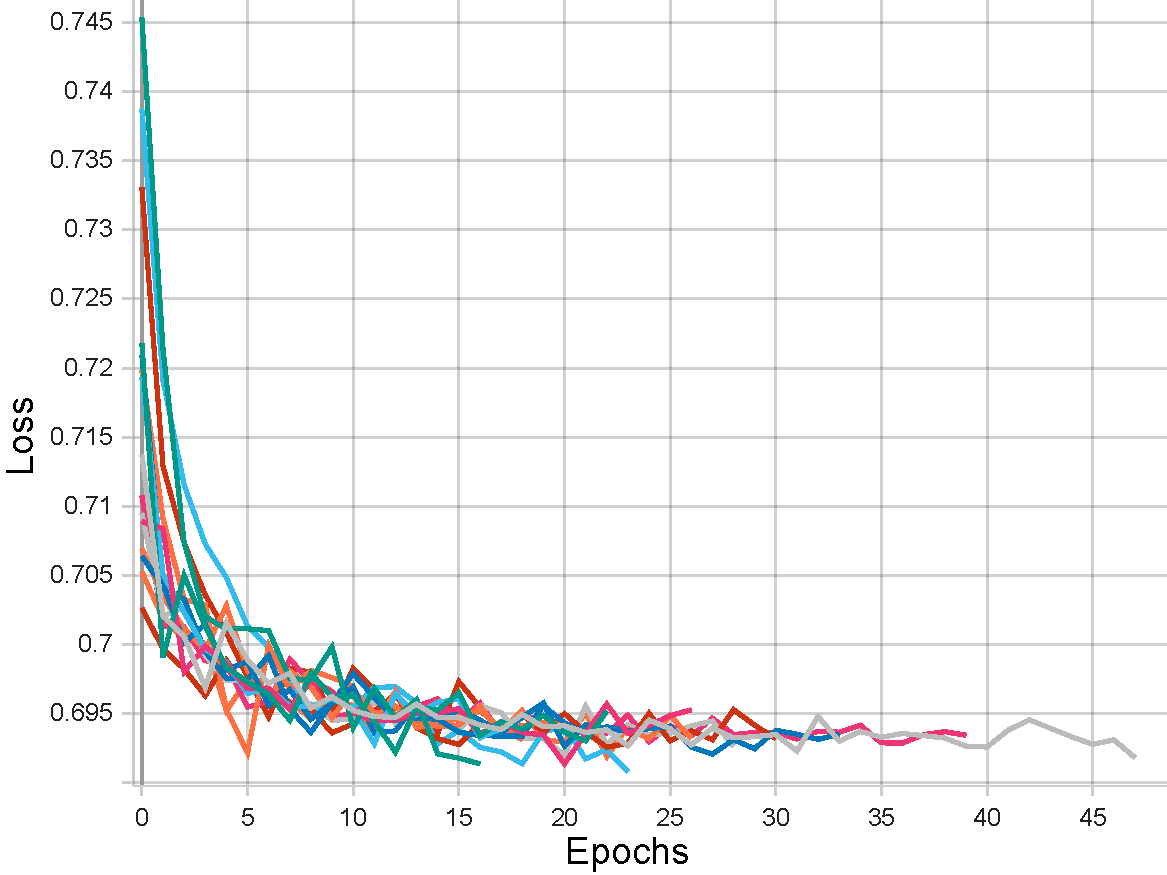
\includegraphics[width=0.575\columnwidth]{figures/results/final/two_days_loss_t.pdf}
    \caption[Training losses for Iteration 5 with two days of historic data]{Figure of all training losses with two days of historic data in Iteration 5}
    \label{fig:iteration5_two_days_train_loss}
\end{figure}
\FloatBarrier

\pagebreak
\textbf{Validation accuracies and losses}
\begin{figure}[ht]
    \centering
    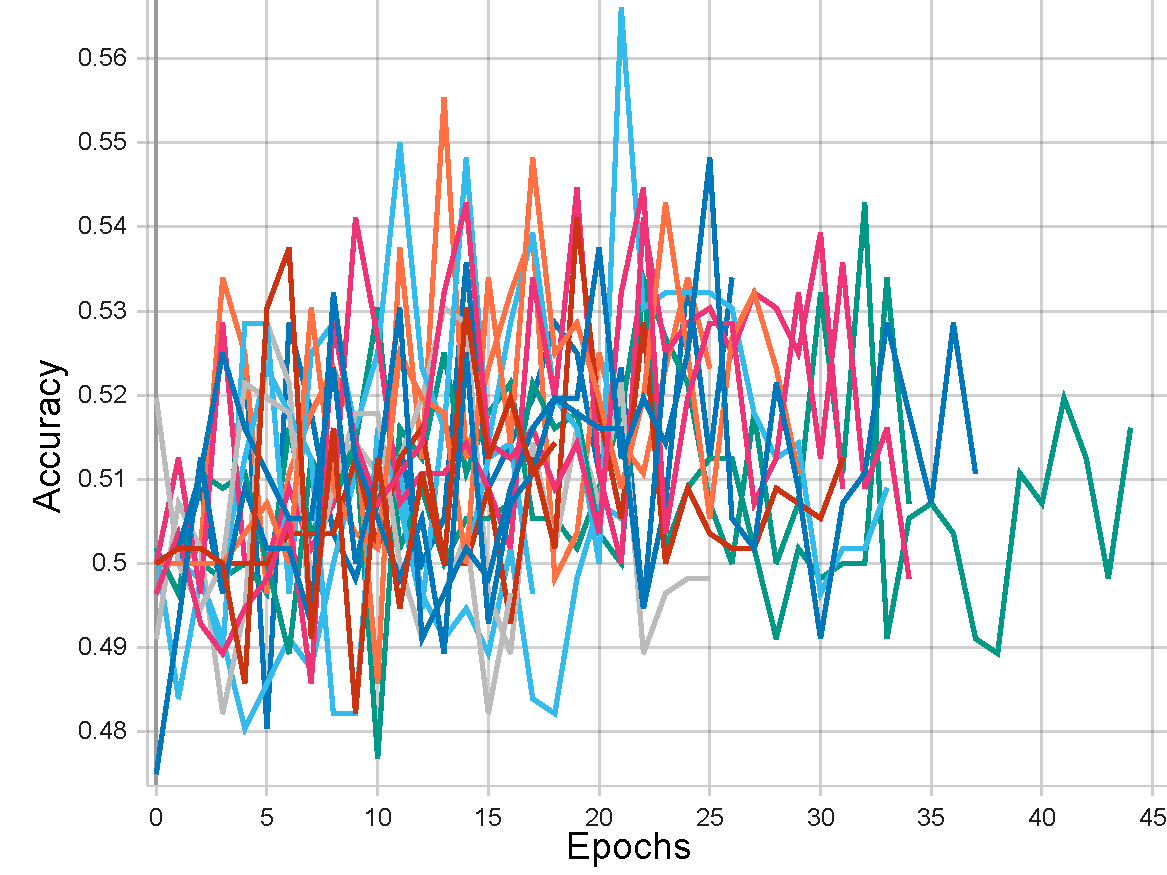
\includegraphics[width=0.575\columnwidth]{figures/results/final/two_days_acc.pdf}
    \caption[Validation accuracies for Iteration 5 with two days of historic data]{Figure of all validation accuracies with two days of historic data in Iteration 5}
    \label{fig:iteration5_two_days_accuracy}
\end{figure}
\FloatBarrier

\begin{figure}[ht]
    \centering
    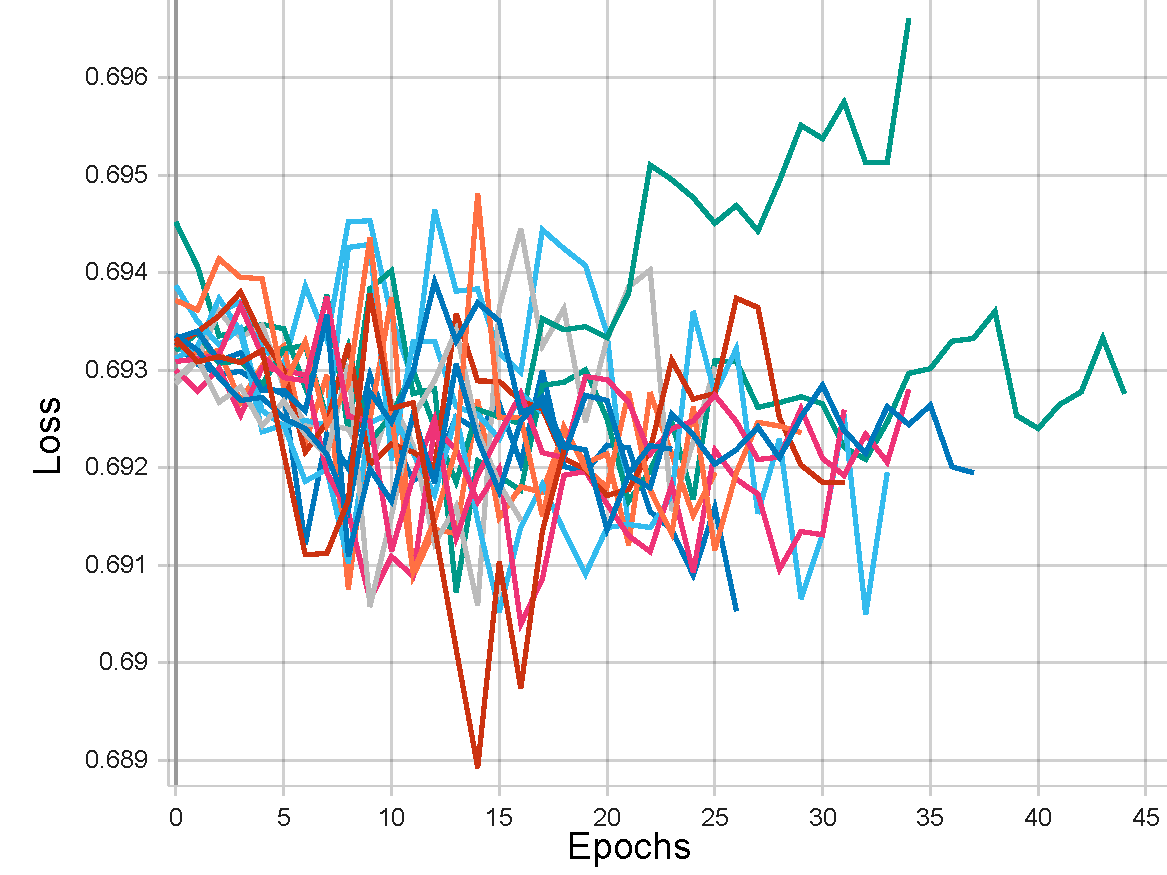
\includegraphics[width=0.575\columnwidth]{figures/results/final/two_days_loss.pdf}
    \caption[Validation losses for Iteration 5 with two days of historic data]{Figure of all validation losses with two days of historic data in Iteration 5}
    \label{fig:iteration5_two_days_loss}
\end{figure}
\FloatBarrier

The greatest validation accuracy for the model with a sequence length of two days was 55.54\% with the dataset using price and volatility data.
While the chart above in \autoref{fig:iteration5_two_days_loss} may look erratic, the changes to the loss are minimal due to the scale as it only varies
between 0.689 and 0.697. This suggests there is little overfitting as it does not increase significantly.

\pagebreak
\subsubsection{One week of historic data accuracies and losses}
\textbf{Training accuracies and losses}
\begin{figure}[ht]
    \centering
    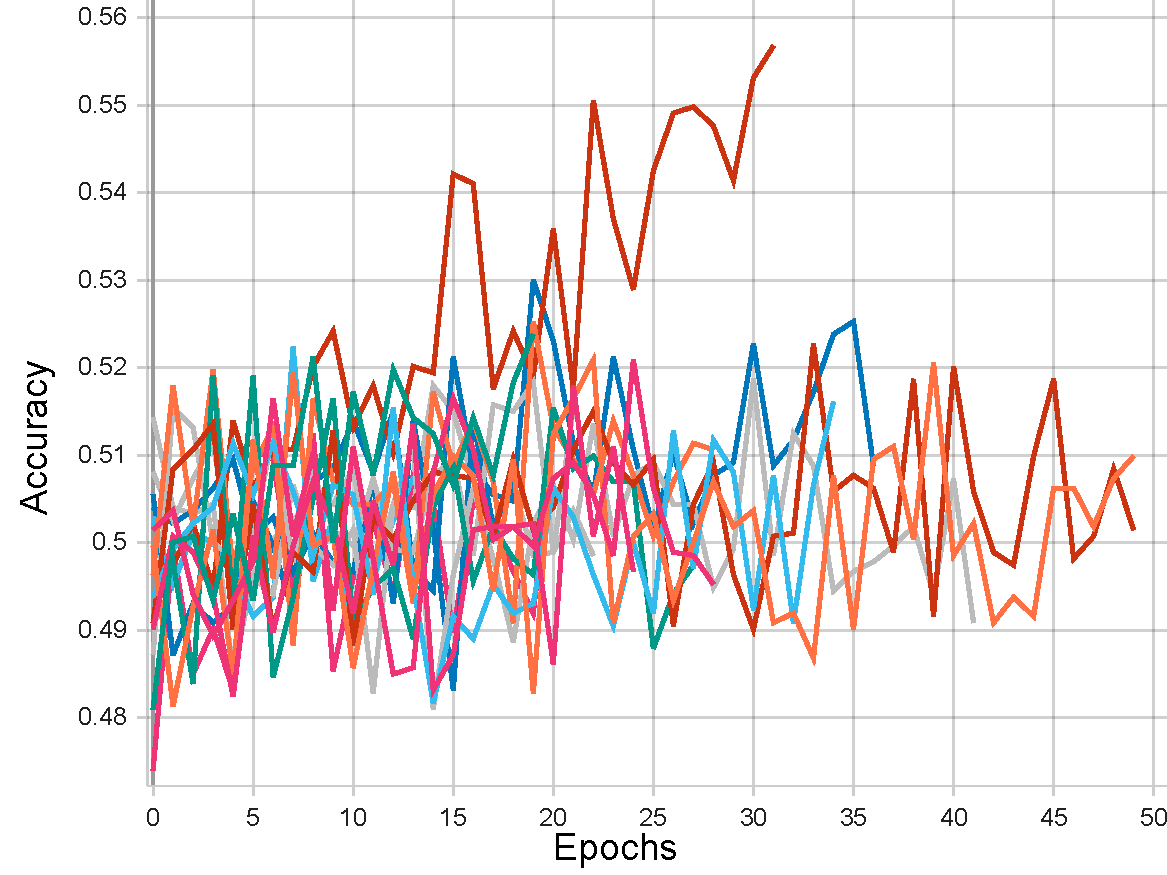
\includegraphics[width=0.575\columnwidth]{figures/results/final/week_acc_t.pdf}
    \caption[Training accuracies for Iteration 5 with one week of historic data]{Figure of all training accuracies with one week of historic data in Iteration 5}
    \label{fig:iteration5_week_train_accuracy}
\end{figure}
\FloatBarrier

\begin{figure}[ht]
    \centering
    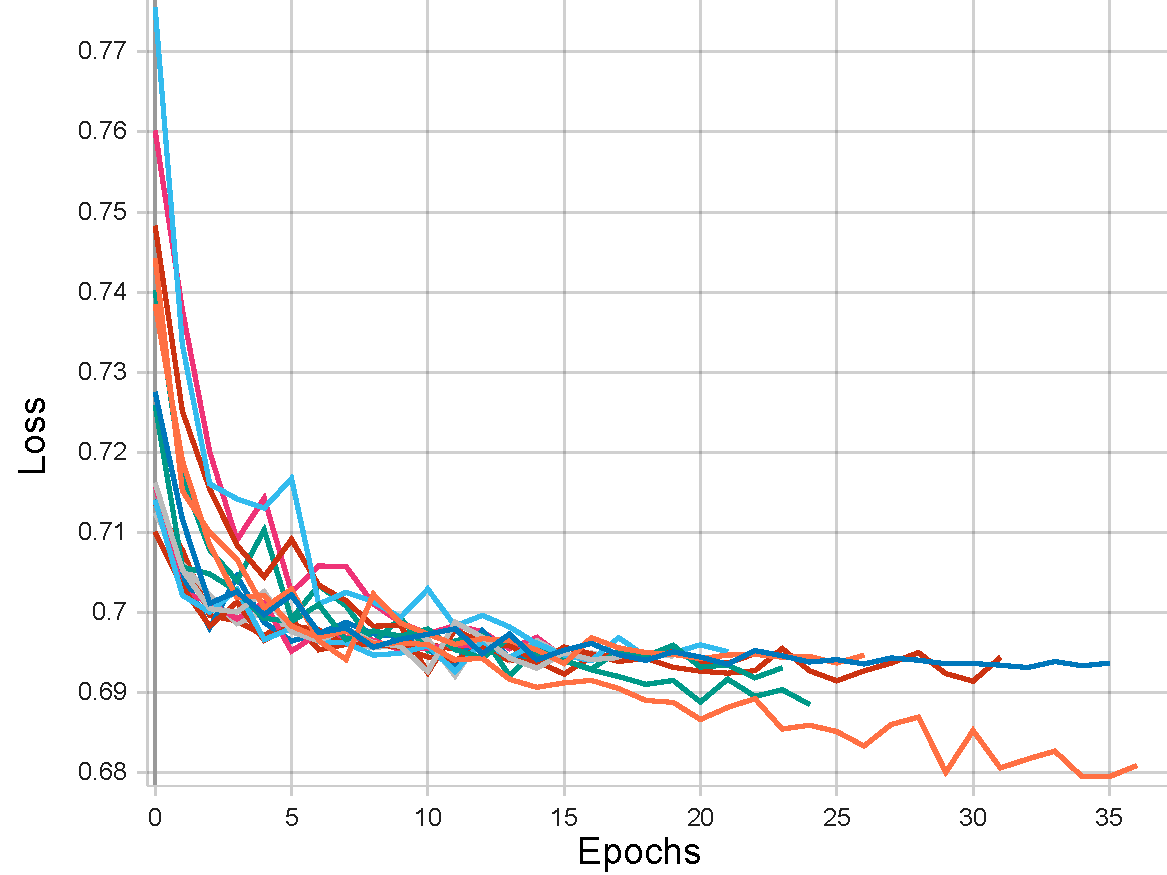
\includegraphics[width=0.575\columnwidth]{figures/results/final/week_loss_t.pdf}
    \caption[Training losses for Iteration 5 with one week of historic data]{Figure of all training losses with one week of historic data in Iteration 5}
    \label{fig:iteration5_week_train_loss}
\end{figure}
\FloatBarrier

\pagebreak
\textbf{Validation accuracies and losses}
\begin{figure}[ht]
    \centering
    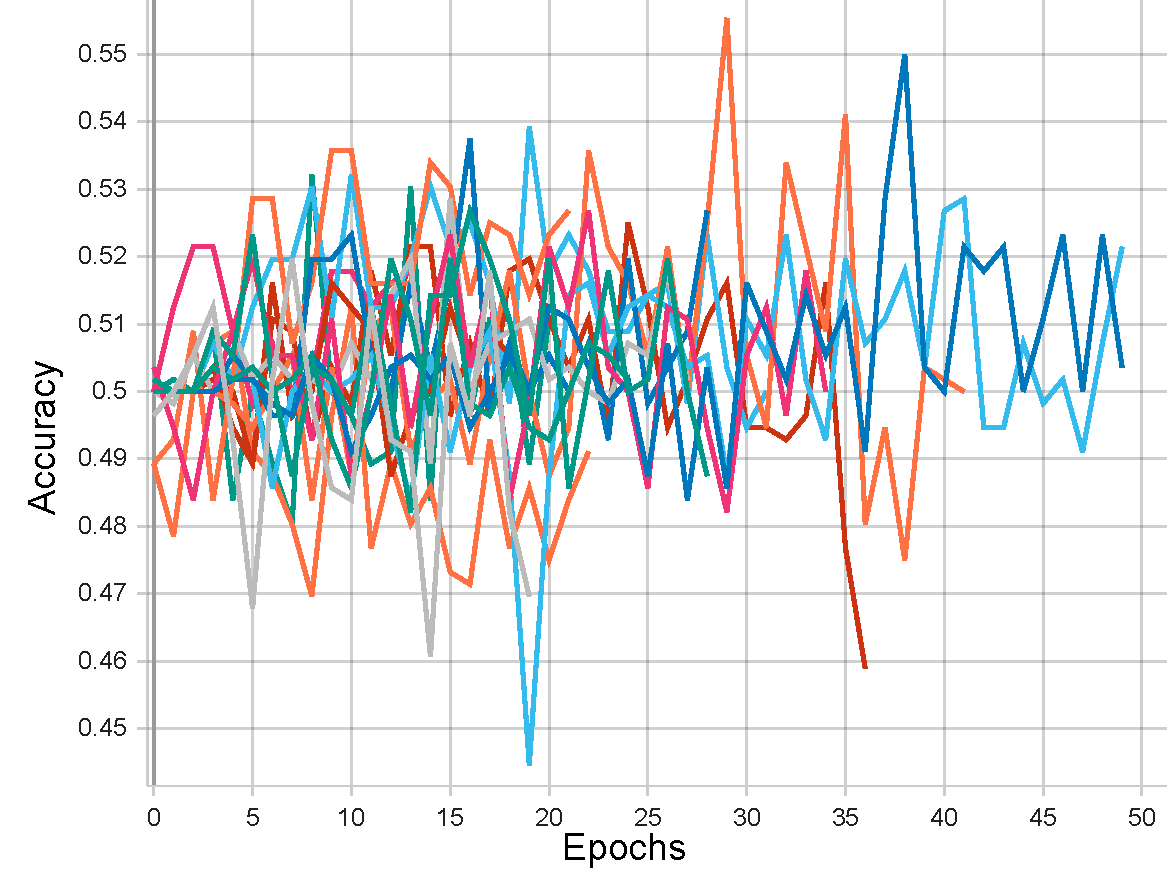
\includegraphics[width=0.575\columnwidth]{figures/results/final/week_acc.pdf}
    \caption[Validation accuracies for Iteration 5 with one week of historic data]{Figure of all validation accuracies with one week of historic data in Iteration 5}
    \label{fig:iteration5_week_accuracy}
\end{figure}

\FloatBarrier
\begin{figure}[ht]
    \centering
    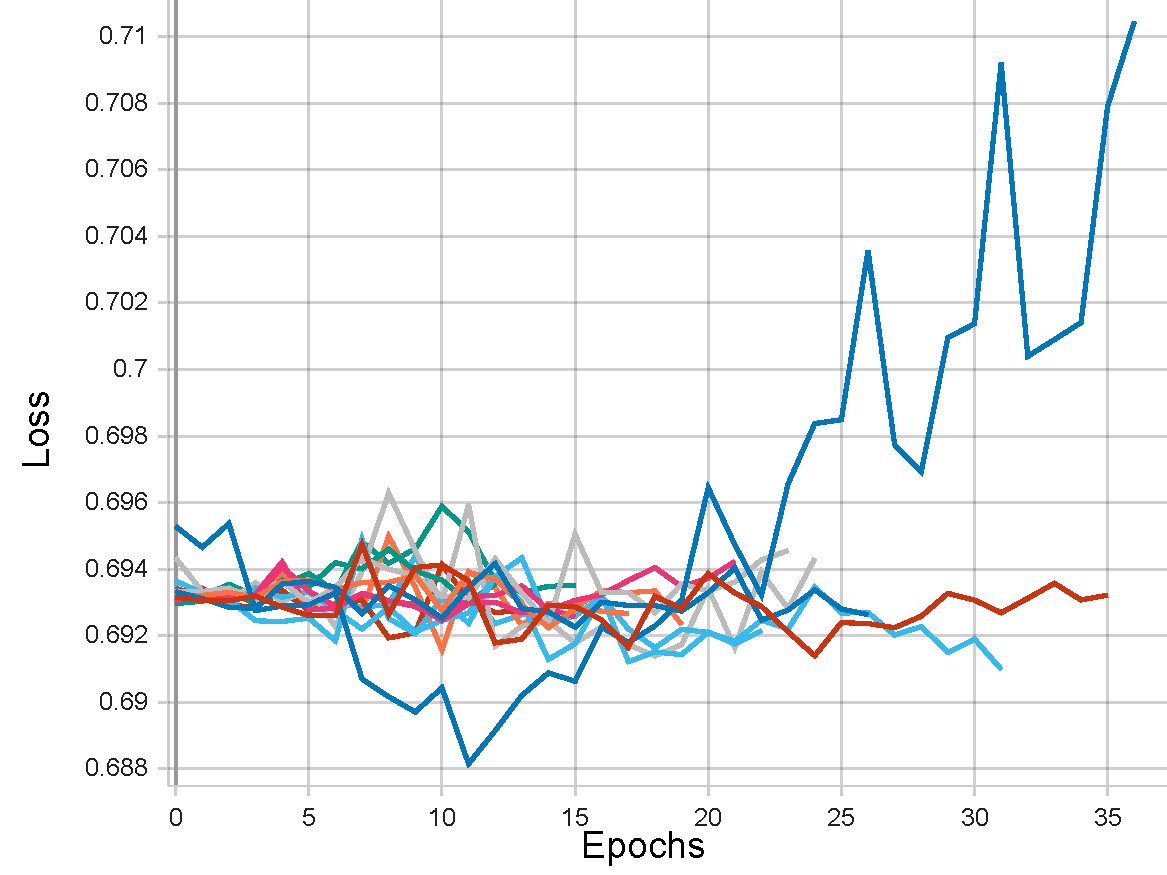
\includegraphics[width=0.575\columnwidth]{figures/results/final/week_loss.pdf}
    \caption[Validation losses for Iteration 5 with one week of historic data]{Figure of all validation losses with one week of historic data in Iteration 5}
    \label{fig:iteration5_week_loss}
\end{figure}
\FloatBarrier

The greatest validation accuracy for the model with a sequence length of one week was 55.54\% with the dataset using price and repurchase
agreements (repo) data.
While the chart above in \autoref{fig:iteration5_week_loss} may look erratic, the changes to the loss are minimal due to the scale as it only varies
between 0.688 and 0.713. This suggests there is little overfitting as it does not increase significantly.

\subsubsection{Two weeks of historic data accuracies and losses}
\textbf{Training accuracies and losses}
\begin{figure}[ht]
    \centering
    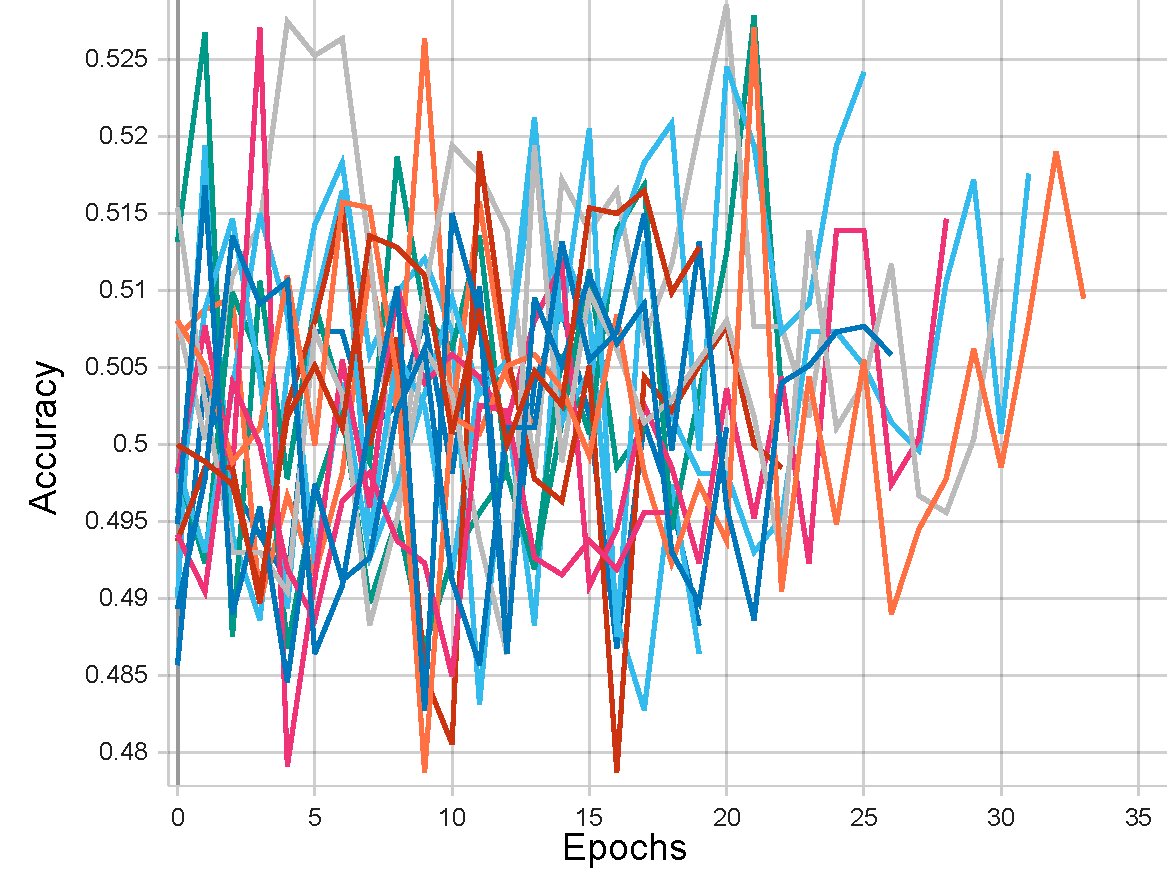
\includegraphics[width=0.575\columnwidth]{figures/results/final/two_weeks_acc_t.pdf}
    \caption[Training accuracies for Iteration 5 with two weeks of historic data]{Figure of all training accuracies with two weeks of historic data in Iteration 5}
    \label{fig:iteration5_two_weeks_train_accuracy}
\end{figure}

\FloatBarrier
\begin{figure}[ht]
    \centering
    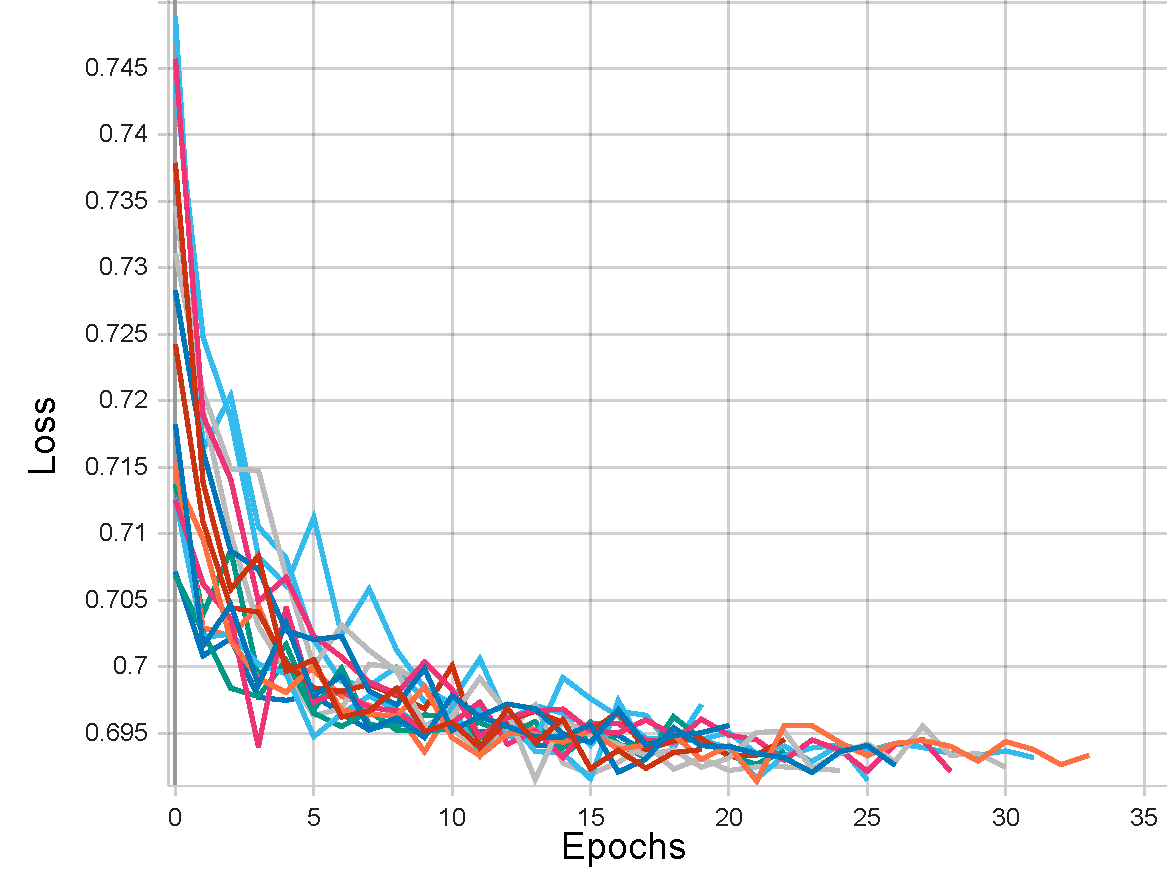
\includegraphics[width=0.575\columnwidth]{figures/results/final/two_weeks_loss_t.pdf}
    \caption[Training losses for Iteration 5 with two weeks of historic data]{Figure of all training losses with two weeks of historic data in Iteration 5}
    \label{fig:iteration5_two_weeks_train_loss}
\end{figure}
\FloatBarrier

\pagebreak
\textbf{Validation accuracies and losses}
\begin{figure}[ht]
    \centering
    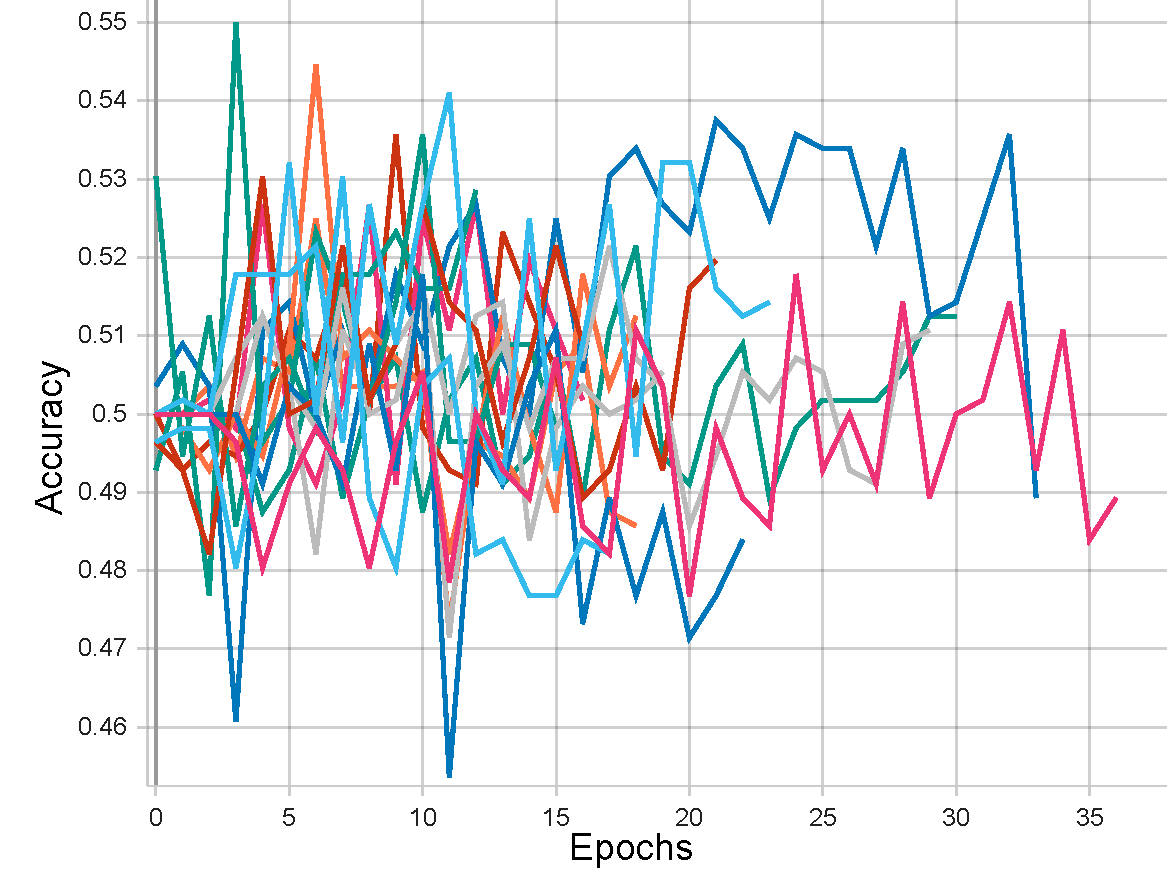
\includegraphics[width=0.575\columnwidth]{figures/results/final/two_weeks_acc.pdf}
    \caption[Validation accuracies for Iteration 5 with two weeks of historic data]{Figure of all validation accuracies with two weeks of historic data in Iteration 5}
    \label{fig:iteration5_two_weeks_accuracy}
\end{figure}
\FloatBarrier

\begin{figure}[ht]
    \centering
    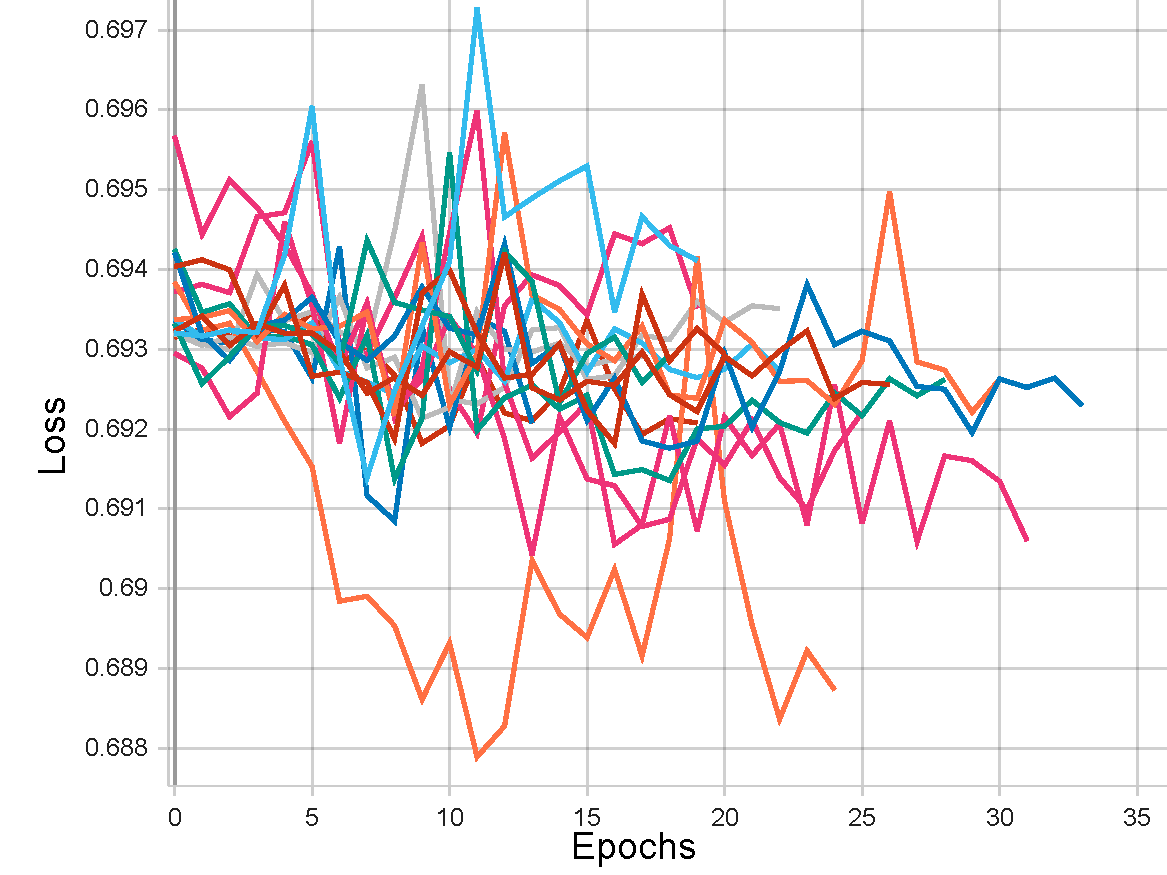
\includegraphics[width=0.575\columnwidth]{figures/results/final/two_weeks_loss.pdf}
    \caption[Validation losses for Iteration 5 with two weeks of historic data]{Figure of all validation losses with two weeks of historic data in Iteration 5}
    \label{fig:iteration5_two_weeks_loss}
\end{figure}
\FloatBarrier

The greatest validation accuracy for the model with a sequence length of two weeks was 55.18\% with the dataset using price and repurchase
agreements (repo) data.
While the chart above in \autoref{fig:iteration5_two_weeks_loss} may look erratic, the changes to the loss are minimal due to the scale as it only varies
between 0.688 and 0.697. This suggests there is little overfitting as it does not increase significantly.

\subsubsection{One month of historic data accuracies and losses}
\textbf{Training accuracies and losses}
\begin{figure}[ht]
    \centering
    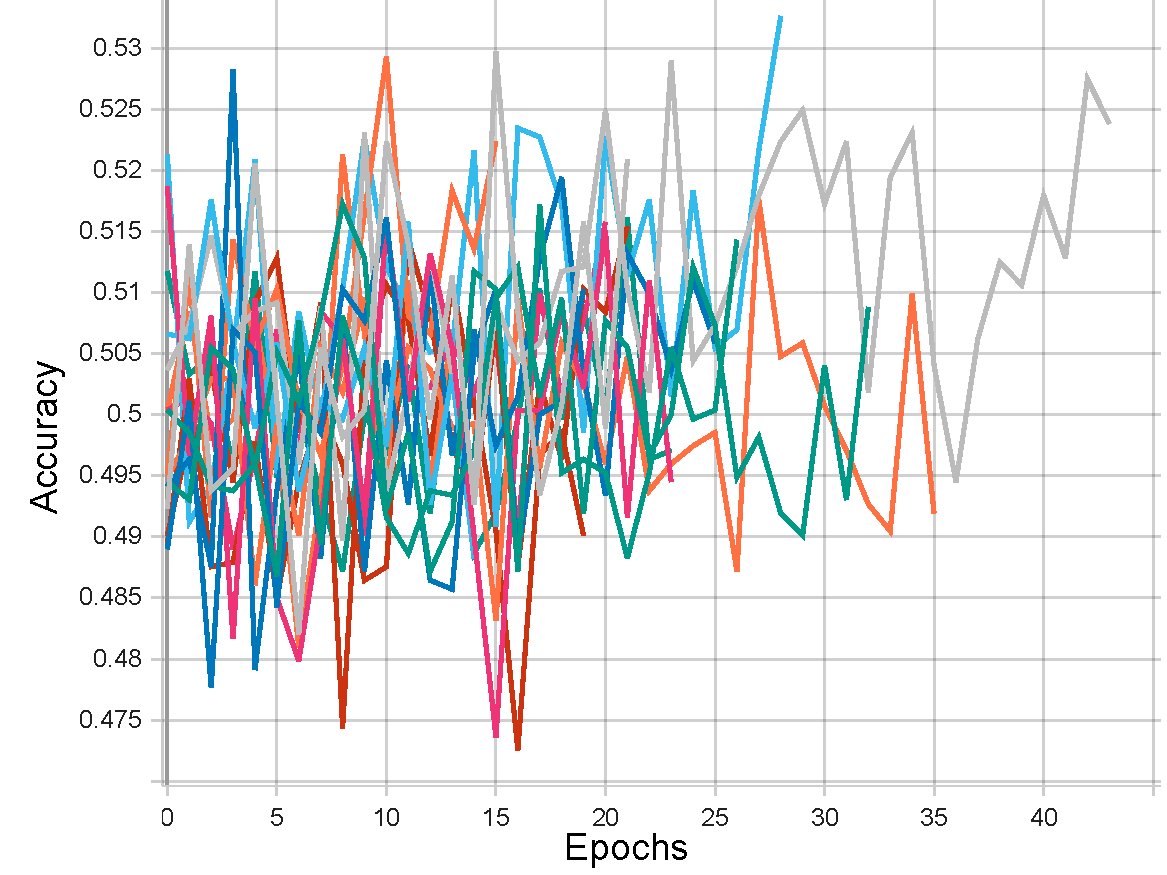
\includegraphics[width=0.575\columnwidth]{figures/results/final/month_acc_t.pdf}
    \caption[Training accuracies for Iteration 5 with one month of historic data]{Figure of all training accuracies with one month of historic data in Iteration 5}
    \label{fig:iteration5_month_train_accuracy}
\end{figure}
\FloatBarrier

\begin{figure}[ht]
    \centering
    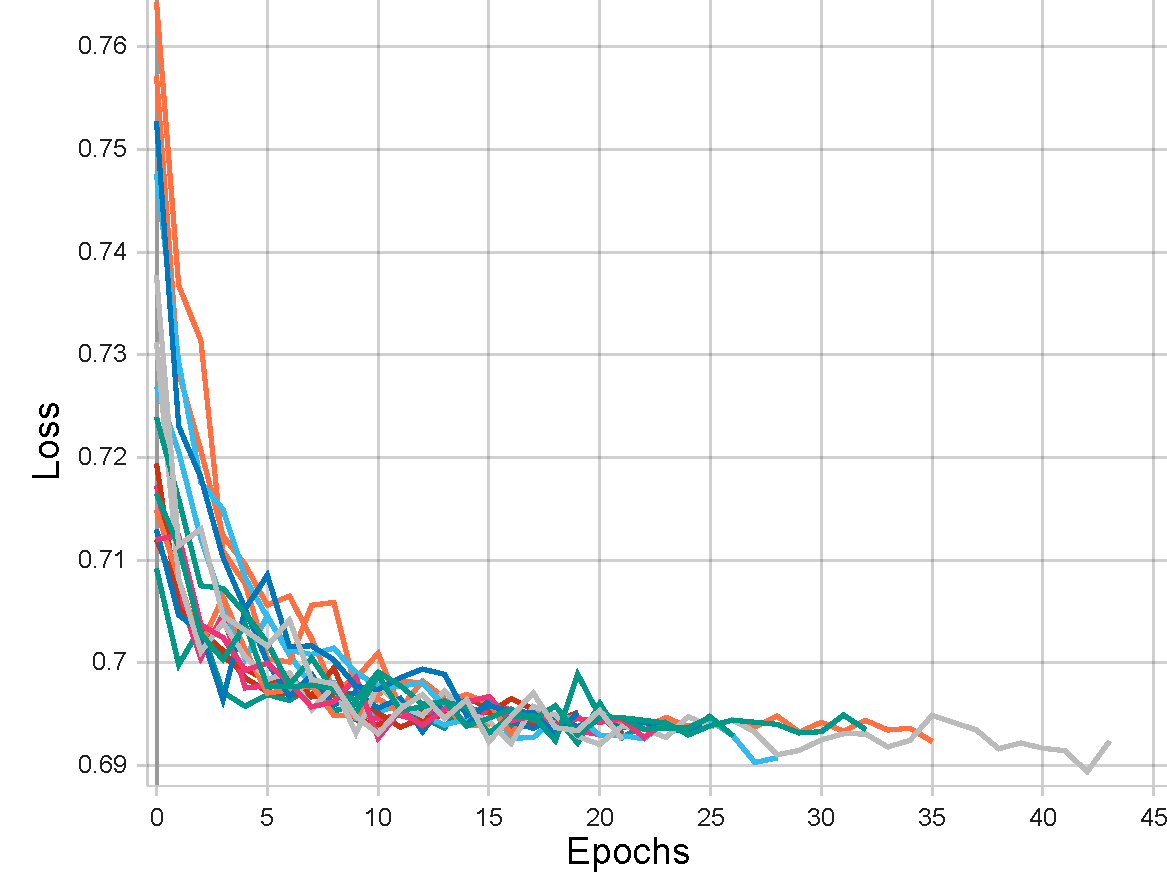
\includegraphics[width=0.575\columnwidth]{figures/results/final/month_loss_t.pdf}
    \caption[Training losses for Iteration 5 with one month of historic data]{Figure of all training losses with one month of historic data in Iteration 5}
    \label{fig:iteration5_month_train_loss}
\end{figure}
\FloatBarrier

\pagebreak
\textbf{Validation accuracies and losses}
\begin{figure}[ht]
    \centering
    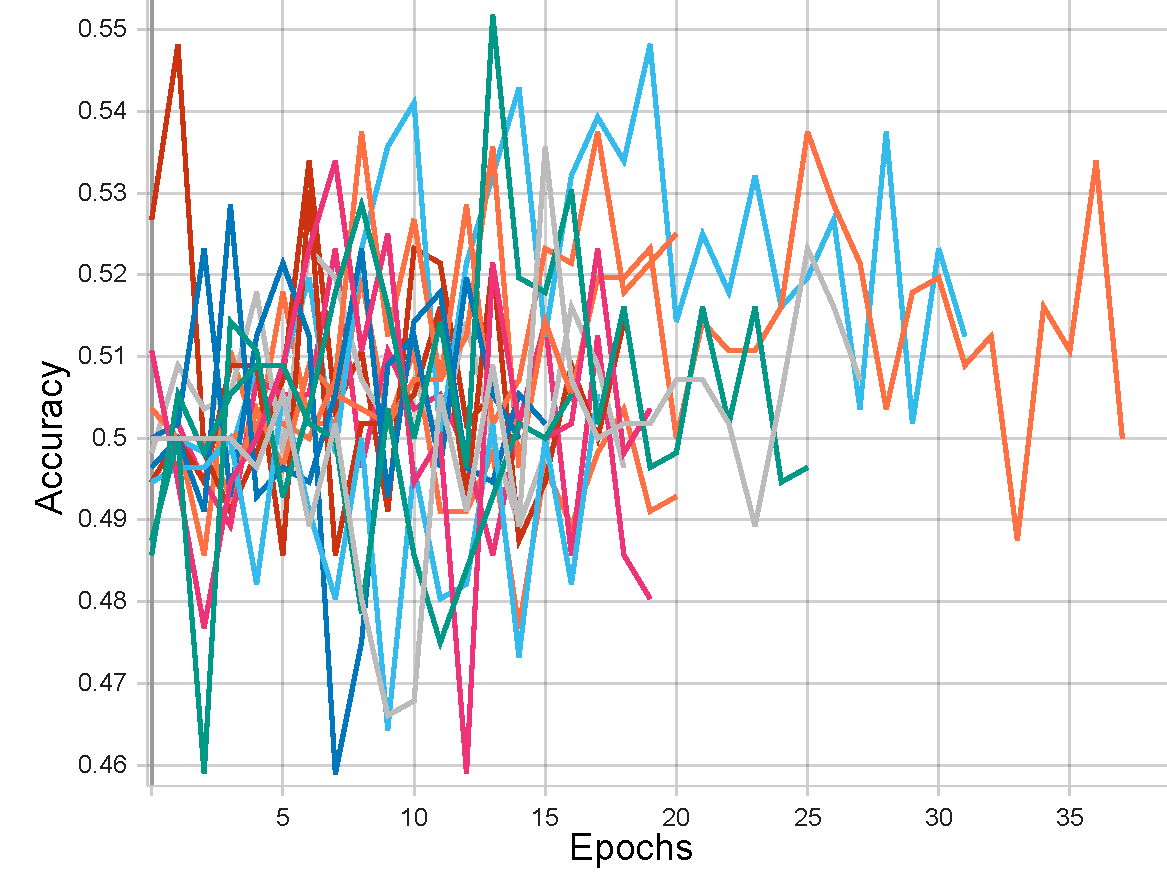
\includegraphics[width=0.575\columnwidth]{figures/results/final/month_acc.pdf}
    \caption[Validation accuracies for Iteration 5 with one month of historic data]{Figure of all validation accuracies with one month of historic data in Iteration 5}
    \label{fig:iteration5_month_accuracy}
\end{figure}
\FloatBarrier

\begin{figure}[ht]
    \centering
    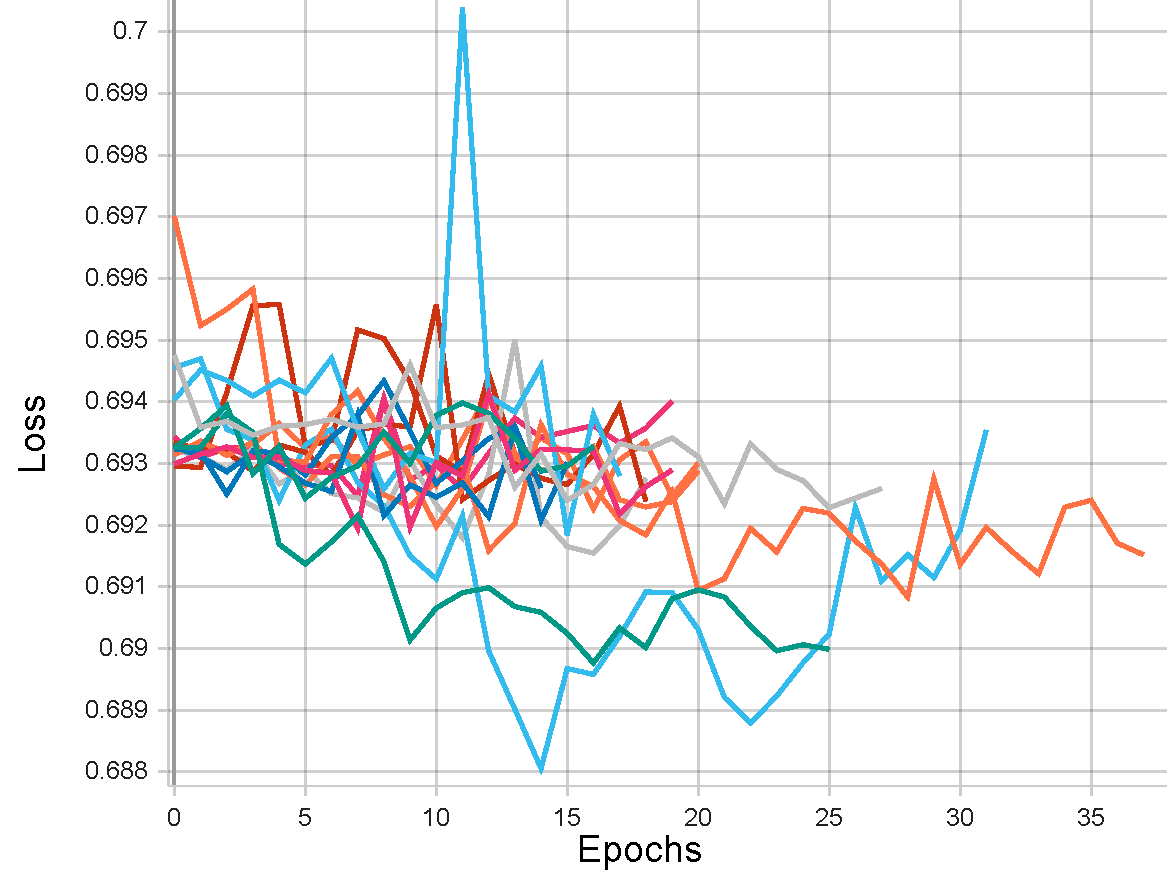
\includegraphics[width=0.575\columnwidth]{figures/results/final/month_loss.pdf}
    \caption[Validation losses for Iteration 5 with one month of historic data]{Figure of all validation losses with one month of historic data in Iteration 5}
    \label{fig:iteration5_month_loss}
\end{figure}
\FloatBarrier

The greatest validation accuracy for the model with a sequence length of two weeks was 57.50\% with the dataset using price
and treasury yields data.
While the chart above in \autoref{fig:iteration5_month_loss} may look erratic, the changes to the loss are minimal due to the scale as it only varies
between 0.687 and 0.696. This suggests there is little overfitting as it does not increase significantly.

\pagebreak
\subsubsection{Two months of historic data accuracies and losses}
\textbf{Training accuracies and losses}
\begin{figure}[ht]
    \centering
    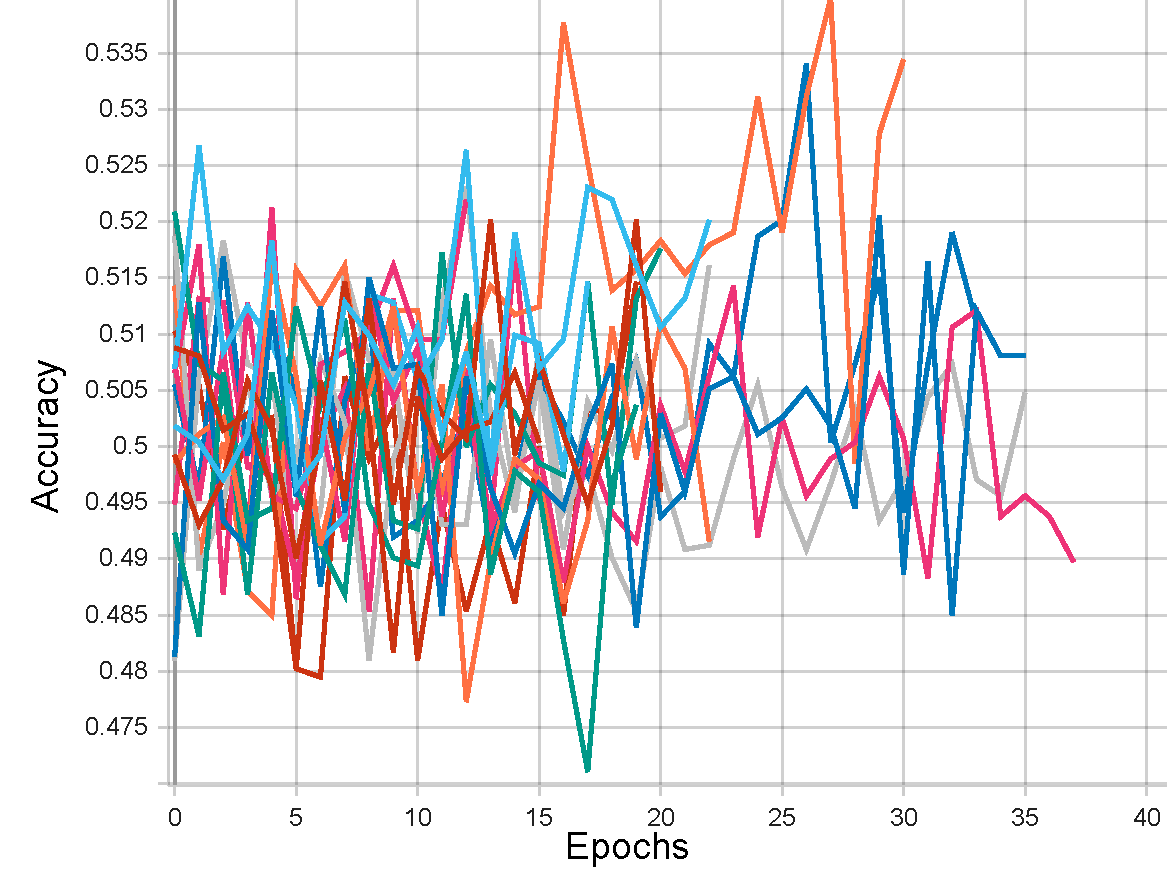
\includegraphics[width=0.575\columnwidth]{figures/results/final/two_months_acc_t.pdf}
    \caption[Training accuracies for Iteration 5 with two months of historic data]{Figure of all training accuracies with two months of historic data in Iteration 5}
    \label{fig:iteration5_two_months_train_accuracy}
\end{figure}
\FloatBarrier

\begin{figure}[ht]
    \centering
    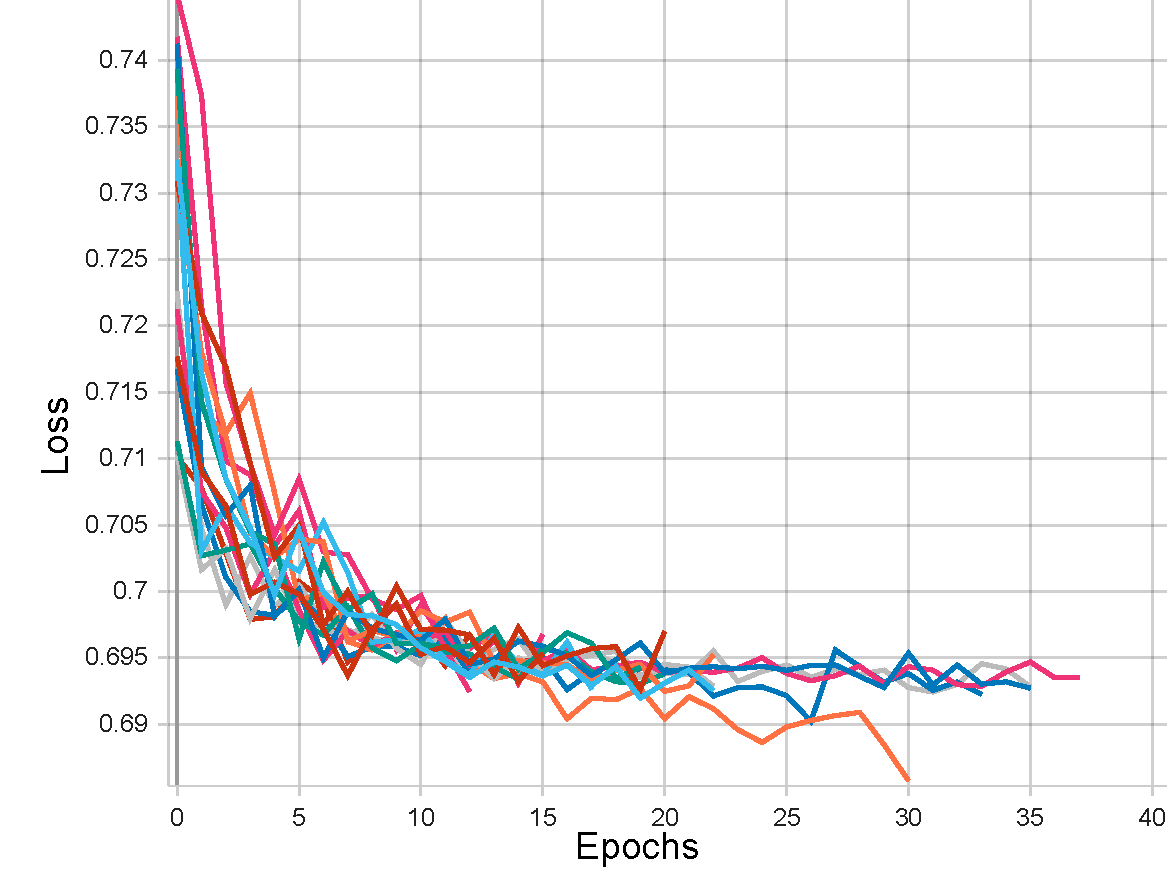
\includegraphics[width=0.575\columnwidth]{figures/results/final/two_months_loss_t.pdf}
    \caption[Training losses for Iteration 5 with two months of historic data]{Figure of all training losses with two months of historic data in Iteration 5}
    \label{fig:iteration5_two_months_train_loss}
\end{figure}
\FloatBarrier

\pagebreak
\textbf{Validation accuracies and losses}
\begin{figure}[ht]
    \centering
    \includegraphics[width=0.575\columnwidth]{figures/results/final/two_months_acc.pdf}
    \caption[Validation accuracies for Iteration 5 with two months of historic data]{Figure of all validation accuracies with two months of historic data in Iteration 5}
    \label{fig:iteration5_two_months_accuracy}
\end{figure}
\FloatBarrier

\begin{figure}[ht]
    \centering
    \includegraphics[width=0.575\columnwidth]{figures/results/final/two_months_loss.pdf}
    \caption[Validation losses for Iteration 5 with two months of historic data]{Figure of all validation losses with two months of historic data in Iteration 5}
    \label{fig:iteration5_two_months_loss}
\end{figure}
\FloatBarrier

The greatest validation accuracy for the model with a sequence length of two weeks was 54.11\% with the dataset using the extended price
changes dataset, the price and volatility data, or the price and treasury yields data.
While the chart above in \autoref{fig:iteration5_two_months_loss} may look erratic, the changes to the loss are minimal due to the scale as it only varies
between 0.689 and 0.703. This suggests there is little overfitting as it does not increase significantly.

\subsubsection{One quarter of historic data accuracies and losses}
\textbf{Training accuracies and losses}
\begin{figure}[ht]
    \centering
    \includegraphics[width=0.575\columnwidth]{figures/results/final/quarter_acc_t.pdf}
    \caption[Training accuracies for Iteration 5 with one quarter of historic data]{Figure of all training accuracies with one quarter of historic data in Iteration 5}
    \label{fig:iteration5_quarter_train_accuracy}
\end{figure}
\FloatBarrier

\begin{figure}[ht]
    \centering
    \includegraphics[width=0.575\columnwidth]{figures/results/final/quarter_loss_t.pdf}
    \caption[Training losses for Iteration 5 with one quarter of historic data]{Figure of all training losses with one quarter of historic data in Iteration 5}
    \label{fig:iteration5_quarter_train_loss}
\end{figure}
\FloatBarrier

\pagebreak
\textbf{Validation accuracies and losses}
\begin{figure}[ht]
    \centering
    \includegraphics[width=0.575\columnwidth]{figures/results/final/quarter_acc.pdf}
    \caption[Validation accuracies for Iteration 5 with one quarter of historic data]{Figure of all validation accuracies with one quarter of historic data in Iteration 5}
    \label{fig:iteration5_quarter_accuracy}
\end{figure}
\FloatBarrier

\begin{figure}[ht]
    \centering
    \includegraphics[width=0.575\columnwidth]{figures/results/final/quarter_loss.pdf}
    \caption[Validation losses for Iteration 5 with one quarter of historic data]{Figure of all validation losses with one quarter of historic data in Iteration 5}
    \label{fig:iteration5_quarter_loss}
\end{figure}
\FloatBarrier

The greatest validation accuracy for the model with a sequence length of two weeks was 55.18\% with the dataset of the price and treasury yields data.
While the chart above in \autoref{fig:iteration5_quarter_loss} may look erratic, the changes to the loss are minimal due to the scale as it only varies
between 0.687 and 0.699. This suggests there is little overfitting as it does not increase significantly.

\subsection{Comparisons of models in iteration 5}\label{ssec:iteration5_best_val_acc}
The table below in \autoref{fig:final_val_accuracy} shows the accuracies of each combination of input features and length of historic data.
\begin{figure}[ht]
    \centering
    \includegraphics[width=0.95\columnwidth]{figures/results/final/final_val_accuracy.pdf}
    \caption[Best validation accuracies for Iteration 5]{Figure of all validation accuracies of each combination of input features and sequence length in Iteration 5}
    \label{fig:final_val_accuracy}
\end{figure}
\FloatBarrier

The results show the model of the stock market index price combined with treasury yield data and 
a sequence length of 1 month (21 days) of historic data, has the best accuracy with a value of
57.50\%.

However, there is additional data that can be inferred from the results. On average, the model with a sequence
length of two days performs the best with a validation accuracy of 53.84\%. This suggests that the stock markets may react
strongest to short term changes. The models' accuracies slightly decrease for the one-week sequence length, and fluctuate
slightly across other sequence lengths but never increase over the model with a sequence length of two days.

On average, the model utilising price and treasury yields data, have the highest average validation accuracy of 54.76\%. This
shows that treasury yields data can be an important factor to stock market returns.

In order to better visualise how different features affect the model, each combination of input features was compared against the `price only' dataset for each sequence length.
The results of these comparisons can be shown in the table below in \autoref{fig:val_accuracy_comparison}.

\begin{figure}[ht]
    \centering
    \includegraphics[width=0.95\columnwidth]{figures/results/final/val_accuracy_comparison.pdf}
    \caption[Best validation accuracies for Iteration 5]{Figure of all validation accuracies of each combination of input features and sequence length in Iteration 5}
    \label{fig:val_accuracy_comparison}
\end{figure}
\FloatBarrier

The model with a sequence length of two days does not see many significant improvements with most combinations of input features.
For sequence lengths, many factors can have a positive impact to the models, the results above show that volume, volatility,
M1 money supply, GDP, Effective Federal Funds Rate (EFFR), gold prices, currency exchange rates, put-to-call ratio (options), and other
sentiment data. Whereas for sequence lengths of one month, there is some overlap of important factors that affect the accuracy of the models.
The factors that impact one month sequence lengths are the extended price dataset, as well as volume, volatility, M1 money supply, GDP, 
treasury yields, EFFR, Repurchase Agreements (Repo) utilisation and rates, Reverse Repo utilisation and rates, gold prices, currency exchange rates,
and put-to-call ratio (options) data.

\subsection{Evaluation of iteration 5}
The results from iteration 5 provided valuable data in order to be able to answer the research questions. With the best model having an accuracy
of 57.50\%, the results suggest that stock market movements are not always truly random and there are factors that affect stock prices. This
final iteration has provided great insight into which input features affect accuracy of stock market predictions the most, as well as what
sequence lengths of historic data as input. This iteration provides a model with greater accuracies than any model prior to it. The models in this
iteration also show very little overfitting as seen in only very minute fluctuations to the validation losses that do not increase significantly.

Due to time constraints and computational complexity, it was not possible to test various different models of different layers and layer sizes
for each combination of input features which may impact the results.

\section{Benchmark application results}\label{benchmark_results}
The benchmark application uses an existing case study of input features and applies it to the existing research method of the CNN-LSTM sequential
model as described in Iteration 3.

\subsection{Accuracies of all tests}
In the charts below, each line represents a different sequence length to the benchmark case study as described in \autoref{ssec:benchmark_input_features}.
For the training and validation accuracy charts, each line has a corresponding line in the loss charts with the same colour.

There are 6 lines in each chart as there were 6 different sequence lengths tested.
\subsubsection{Training accuracies and losses}
\begin{figure}[ht]
    \centering
    \includegraphics[width=0.95\columnwidth]{figures/results/benchmark/benchmark_all_acc_t.pdf}
    \caption[Training accuracies for Benchmark Model]{Figure of all training accuracies of the different sequence lengths in the Benchmark Model}
    \label{fig:benchmark_train_accuracy}
\end{figure}
\FloatBarrier

\begin{figure}[ht]
    \centering
    \includegraphics[width=0.95\columnwidth]{figures/results/benchmark/benchmark_all_loss_t.pdf}
    \caption[Training losses for benchmark model]{Figure of all training losses of the different sequence lengths in the benchmark model}
    \label{fig:benchmark_train_loss}
\end{figure}
\FloatBarrier

\subsubsection{Validation accuracies and losses}
\begin{figure}[ht]
    \centering
    \includegraphics[width=0.95\columnwidth]{figures/results/benchmark/benchmark_all_acc.pdf}
    \caption[Validation accuracies for benchmark model]{Figure of all validation accuracies of the different sequence lengths in the benchmark model}
    \label{fig:benchmark_all_accuracy}
\end{figure}
\FloatBarrier

\begin{figure}[ht]
    \centering
    \includegraphics[width=0.95\columnwidth]{figures/results/benchmark/benchmark_all_loss.pdf}
    \caption[Validation losses for benchmark model]{Figure of all validation losses of the different sequence lengths in the benchmark model}
    \label{fig:benchmark_all_loss}
\end{figure}
\FloatBarrier



\subsection{Accuracies of the best result}

\begin{figure}[ht]
    \centering
    \includegraphics[width=0.95\columnwidth]{figures/results/benchmark/benchmark_quarter_acc.pdf}
    \caption[Best accuracy for the benchmark model]{Figure of the best accuracy of the different sequence lengths in the benchmark model}
    \label{fig:benchmark_best_accuracy}
\end{figure}
\FloatBarrier

\begin{figure}[ht]
    \centering
    \includegraphics[width=0.95\columnwidth]{figures/results/benchmark/benchmark_quarter_loss.pdf}
    \caption[Best loss for the benchmark model]{Figure of the best loss of the different sequence lengths in the benchmark model}
    \label{fig:benchmark_best_loss}
\end{figure}
\FloatBarrier

The blue line represents the training set and the pink line represents
the validation set. The validation loss shows little overfitting as can be seen in
\autoref{fig:benchmark_best_loss} as the loss does not significantly increase. At 10 epochs,
the validation accuracy reaches its highest value of 54.55\% whilst the training accuracy reached 50.18\%. The validation accuracy being somewhat greater than the
training accuracy can be explained by the dropout layers within the model that can affect the results of the training
set but does not affect the validation set.


\subsection{Evaluation of benchmark model}
The benchmark model utilises an existing case study as noted in \autoref{ssec:benchmark_input_features}
With a validation accuracy of 54.55\%, there is an improvement above a random guess of the direction
of the next trading day. This model was included to compare the results of the models of the artefact to understand
how well it performs to existing models.  This result suggests that the models of all five iterations of the artefact
outperform the existing case study as described in \autoref{ssec:benchmark_input_features}.

The LSTM model in Iteration 1, CNN-LSTM sequential models in Iteration 3 and 5 outperform this benchmark model
with validation accuracies of 55.54\%, 56.07\% and 57.50\% respectively.


\section{Artefact evaluation}
The artefact in this project is shown to be novel based on the unique sets of input features as
it is the first time application of a novel case study to an existing research method. Generally,
the results from the models shown have been able to support in answering the research questions.

\subsection{Research questions evaluation}
\hyperref[predicting_direction_question]{\textbf{Question 1: Predicting a stock market index's direction}}


The results from the artefact suggest that it is possible to predict the stock market index's direction
with a reasonable degree of accuracy. The best model of Iteration 5 had a validation accuracy of 57.5\%
which suggests there is often an ability to predict the daily direction of a stock market index. This
may also suggest there are often inefficiencies in the market and may offer some evidence to disprove
the efficient market hypothesis. While this model has been quite accurate, there are some limitations
involved that may affect the accuracy. The model uses data from November 2006 to March 2022; this involves
a relatively large time horizon and as a result, some ideas learned by the model may be outdated as the markets
evolve over time; for example settlement periods adjusting from T+3 days to T+2 days.

\hyperref[optimal_historical_question]{\textbf{Question 2: Optimal amount of historical data as input}}

The results from the artefact generally show that one month of historical data can provide the best models as seen in \autoref{fig:val_accuracy_comparison};
though for the input features tested, two days has the best results when averaged as the results show in \autoref{fig:final_val_accuracy}.
Generally, a short sequence length of historical data provides
the best result for predicting the daily direction of the stock market index with few input features affecting the accuracy of the
model. However, given an optimal set of input features, the model may be able to recognise patterns in longer sequence lengths.

The two day sequence length may be more accurate due to the fact markets are always adjusting and reacting to changes; and as a result
there may be short term inefficiencies that can be exploited. However, the one month sequence length accuracies may be explained due to
the fact many economic factors are reported by institutions / governments on a monthly basis. Furthermore, the one month sequence length
may be the best length for the LSTMs in the neural network model to identify and remember patterns that are beneficial to the model and
disregard any patterns that provide less value.

\hyperref[most_important_features_question]{\textbf{Question 3: Most important input features}}

The results are significantly more nuanced and cannot be placed into neat categories as described in \autoref{ssec:input_feature_chosen}.
On average, including treasury yields data to the model improved accuracies by 3.17\% compared to price alone as seen in
\autoref{fig:val_accuracy_comparison}.
The artefact suggests that information regarding the treasury yields have the most impact to the neural network models across all sequence
lengths apart from two days. 
This is likely due to the fact there generally aren't significant changes to treasury yields in a two-day period; but they can
grow to be more significant over a long time horizon. The increased accuracy is likely due to the changes in yields may affect institutional decisions
depending on the risk management. Firms may reallocate funds between the stock market and treasury products; treasury products are generally less risky but
offer lesser returns than the stock market. Repurchase agreements (repos) show trends similar to the treasury yields. There generally aren't significant
changes in 2 days, but there may be patterns over longer periods of times. This may be due to the fact changes to repo markets
can affect liquidity in other markets.

There are several factors that do not impact the model greatly, such as reverse repurchase agreements (reverse repos).
This is likely due to the fact reverse repos were generally underutilised, especially in the training period and as a result did 
not affect the model significantly. Exchange volume, gold, currency exchange rates, inflation rates, and employment rates
generally did not affect the accuracy significantly. This is likely due to those factors remaining relatively stable most of the time.

\subsection{Requirements evaluation}
\subsubsection{Functional requirements}
\textbf{Necessary functional requirements}
\begin{table}[ht]
    \centering
    \begin{tabular}{|p{100mm}|c|}
        \hline
        Requirement & Met? \\
        \hline\hline
        Predict daily price direction with 60\%+ accuracy & No \\
        Identify which input features are the most important & Yes \\
        Identify what sequence length (number of days of history of each input feature) is optimal & Yes \\
        Present charts of accuracies and losses of each model & Yes \\
        \hline
    \end{tabular}
    \caption{Table showing whether necessary functional requirements were met}
    \label{tab:necessary_functional_requirements}
\end{table}
\FloatBarrier

Unfortunately, the models were not able to provide an accuracy greater than 60\%, but this did not
affect the models' ability to identify optimal features in stock market forecasting. Charts were
also able to produced using the Tensorboard callback.

\textbf{Optional functional requirements}
\begin{table}[ht]
    \centering
    \begin{tabular}{|p{100mm}|c|}
        \hline
        Requirement & Met? \\
        \hline\hline
        Predict daily price return with a mean absolute deviation of 2.5\% or lower & No \\
        \hline
    \end{tabular}
    \caption{Table showing whether optional functional requirements were met}
    \label{tab:optional_functional_requirements}
\end{table}
\FloatBarrier

This requirement was not met due to time constraints and decisions to focus on other models
predicting direction only. This decision was made due to the belief that understanding
the direction is more important than specific prices to generate a positive return on investment.

\subsubsection{Non-functional requirements}
\textbf{Necessary non-functional requirements}
\begin{table}[ht]
    \centering
    \begin{tabular}{|p{100mm}|c|}
        \hline
        Requirement & Met? \\
        \hline\hline
        The artefact should take less than one minute to run per model chosen (on modern Nvidia GPUs) & Yes* \\
        \hline
    \end{tabular}
    \caption{Table showing whether necessary non-functional requirements were met}
    \label{tab:necessary_non_functional_requirements}
\end{table}

*All models apart from concatenated parallel hybrid models were able to train the models in under a minute.
The models in Iteration 4 were not chosen to be used in the final iteration due to poor accuracies.
\begin{figure}[ht]
    \centering
    \includegraphics[width=0.95\columnwidth]{figures/time_taken.png}
    \caption[Time taken to train models]{Figure comparing the time taken to train models in Iteration 5 compared to Iteration 4}
    \label{fig:time_take_for_models}
\end{figure}
\FloatBarrier

\textbf{Optional non-functional requirements}
\begin{table}[ht]
    \centering
    \begin{tabular}{|p{100mm}|c|}
        \hline
        Requirement & Met? \\
        \hline\hline
        Front-end application that allows users to input features and sequence lengths to train different models & No \\
        User-facing documentation for artefact & No \\
        \hline
    \end{tabular}
    \caption{Table showing whether optional non-functional requirements were met}
    \label{tab:optional_non_functional_requirements}
\end{table}

Due to time constraints these requirements were not completed. Due to this being primarily a research project
rather than an engineering project, it was deemed unnecessary to have a front-end application. It is relatively
easy to adjust different models with the python code provided. The code also contains comments throughout and uses
relevant variable names to ensure readability and understanding. Furthermore, Tensorboard provides a good front-end
for visualising performance metrics of the models.
\chapter{Project Management} \label{chap:project-management}

\chapter{Conclusion} \label{chap:conclusion}
\section{Overview}
This project highlights the debate concerning the efficient market hypothesis and the feasability
of predicting stock markets, particularly the US stock market. This debate is likely to continue 
for many years to come, but the project shows some evidence of market inefficiencies in short term
horizons that neural networks can detect from both short-term and mid-term sequence lengths.
This project looks at the performance of a few neural network models including Convolutional Neural
Networks (CNNs), Long-Short Term Memory networks (LSTMs) and hybrid approachs (CNN-LSTMs).

The artefact generated in this project has a meaningful accuracy in stock market forecasting,
and the results from final iteration have been able to aid in optimal feature selection in terms
of input features and sequence lengths. The results of the models can be used to aid investors'
decisions in what factors they focus on when making investment decisions as well as to allow
investors to potentially take advantage of market inefficiencies.

\section{Future Work}
For the future, additional input features or different combinations of input features can be tested
on the same research method to identify if there are opportunities for further optimisations.
Furthermore, the same input features can be tested on different research models to verify the results
of the optimal feature selection identified in this project. With an increased amount of time, or with
more powerful hardware, additional neural network parameters such as the layer sizes and amounts can be
tested to identify if there are better performing models.

While this project was not able to identify specific future prices of the stock market, that is an
area that can be looked into further utilising the factors identified in this project. This could be
helpful specifically to the options market where specific prices are important to participants.

Additionally, as this project identifies some input features are more or less important depending on
the sequence length of historical data; an approach to exploit the advantages of different
sequence lengths could prove to produce a model with greater accuracy.

% 
\chapter{More examples}

\section{Equations}

Here's an equation,
\begin{equation}
E=mc^2.\label{eq:einstein}
\end{equation}

\noindent I can reference that easily in the text: \autoref{eq:einstein}. It's even a hyperlink. How nice. 

\section{Opening and closing quotes}

Unlike modern word processors, you need to specify in \LaTeX{} which quote mark to print. To get an opening quote you use a backtick and the regular apostrophe for a closing quote. Double them up for speech. ``This isn't so hard after all''. One just needs to `get used' to it. 

One should never use an apostrophe for plurals. Nope, not even for abbreviations, e.g. in the 1990s, people bought CDs from Virgin Megastores. 

In the \textbf{extremely} rare cases where it's unclear, match it with an opening quote if you must. I got three `A's for my AS Levels. 

\section{Tables}

Tables are joyous fun. The \verb+tabular+ environment is the most common, although it's rather old fashioned and wrangling it into doing what you want can be arcane. Happily, tablesgenerator.com can produce tables from a visual editor or paste from word.

A few things to help you unlearn bad table habits:

\begin{itemize}
    \item You should not use vertical lines in tables. Seriously -- this is an awful 1990s era default from Microsoft Word which has hung around and never gone away. 
    \item the booktabs package can make prettier tables (vertical lines are intentionally banned) - select this option in tablesgenerator. I have included the package for you
    \item You should use tables for comparing numerical data and not as a way of laying out content or paragraph text
\end{itemize}

\begin{table}
    \centering
    \begin{tabular}{lccc}
        \toprule
        \textbf{Feature} & \textbf{Liked (\%)} & \textbf{Disliked (\%)} & \textbf{Didn't know (\%)}  \\ \midrule
        Vertical lines & 0 & 90 & 10 \\
        Using Word & 40 & 40 & 20 \\
        \bottomrule
    \end{tabular}
    \caption{Made up percentages of participants that liked random features}
    \label{tab:sample}
\end{table}

\noindent \autoref{tab:sample} shows a simple table made by hand by yours truly. Note that the column separator is \& which means you must always escape that character if you want to use it in text.






%%%%%%%%%%%%%% REFERENCES SECTION
\newpage
\phantomsection
\addcontentsline{toc}{chapter}{References}
% In order to try and get a consistent format I copy and paste the INSPIRE bibtex code into my bibtex file.
\printbibliography

%%%%%%%%%%%%%%% APPENDICES
\appendix
\chapter{PID}
The scope of the project has changed since the PID due to a number of reasons. Primarily the project
type was adjusted from engineering to research and as a result the requirements of the project had changed.
The project had become more focused on answering research questions rather than building an artefact.
\includepdf[pages=-]{appendices/UP893057_PID.pdf}

\chapter{Ethics Review}
\includepdf[pages=-]{appendices/EthicsReview.pdf}

\chapter{Source Code}
The source code for this project is available in the main.ipynb and benchmark.ipynb files in this
public GitHub repository: \url{https://github.com/Alvie/predicting-stocks-fyp}.



\end{document}
